\PassOptionsToPackage{table}{xcolor}
\documentclass[fleqn,10pt]{wlscirep}
\usepackage[utf8]{inputenc}
\usepackage[T1]{fontenc}
\usepackage{xcolor}
\usepackage{colortbl}
\usepackage{booktabs}
\usepackage{tabularx}
\usepackage{array}
\usepackage{makecell}
\usepackage{graphicx}
\usepackage{subcaption}
\usepackage{float}
\usepackage[section]{placeins}
\usepackage{amsmath,amssymb,amsfonts}
\usepackage{bm}
\usepackage{enumitem}
\usepackage{multirow}
\usepackage{longtable}
\usepackage{threeparttable}
\usepackage{siunitx}
\usepackage{setspace}

\newcolumntype{Y}{>{\raggedright\arraybackslash}X}
\newcommand{\SIplaceholder}[2][0.22\textheight]{%
  \fbox{\parbox[c][#1][c]{0.94\linewidth}{\centering #2}}%
}
\newcommand{\SIfig}[3][0.22\textheight]{%
  \IfFileExists{#2}{%
    \includegraphics[width=\linewidth,height=#1,keepaspectratio]{#2}%
  }{%
    \SIplaceholder[#1]{#3}%
  }%
}
\newcommand{\SIfigalt}[4][0.22\textheight]{%
  \IfFileExists{#2}{%
    \includegraphics[width=\linewidth,height=#1,keepaspectratio]{#2}%
  }{%
    \IfFileExists{#3}{%
      \includegraphics[width=\linewidth,height=#1,keepaspectratio]{#3}%
    }{%
      \SIplaceholder[#1]{#4}%
    }%
  }%
}
\newcommand{\SIEndSection}{\FloatBarrier\clearpage}
\newcommand{\erank}{\operatorname{erank}}
\newcommand{\QZR}{\mathrm{QZR}_{\mathrm{nz}}}
\newcommand{\ODR}{\mathrm{ODR}}

\definecolor{HeadGray}{RGB}{245,245,245}
\definecolor{LoRACol}{RGB}{232,246,255}
\definecolor{TTCol}{RGB}{245,236,255}
\definecolor{LRTTCol}{RGB}{235,255,238}

\renewcommand{\thefigure}{S\arabic{figure}}
\renewcommand{\thetable}{S\arabic{table}}
\renewcommand{\theequation}{S\arabic{equation}}
\renewcommand{\thesection}{S\arabic{section}}
\setcounter{figure}{0}
\setcounter{table}{0}
\setcounter{equation}{0}
\setcounter{secnumdepth}{1}
\setcounter{tocdepth}{1}

\microtypesetup{nopatch=footnote}
\hbadness=10000
\begin{document}

% Blinded standalone SI: the manuscript title and author block are intentionally omitted.
\begin{center}
{\Large\bfseries Supplementary Information}
\end{center}

\vspace{0.5em}
\tableofcontents
\vspace{0.75em}

%====================================================
\clearpage
\section{Electrical Characteristics of the 6T1C Devices: Retention and Update Behavior Across the 5x5 Array}
\label{sec:S1}
%====================================================

\begin{figure}[!htbp]
  \centering
  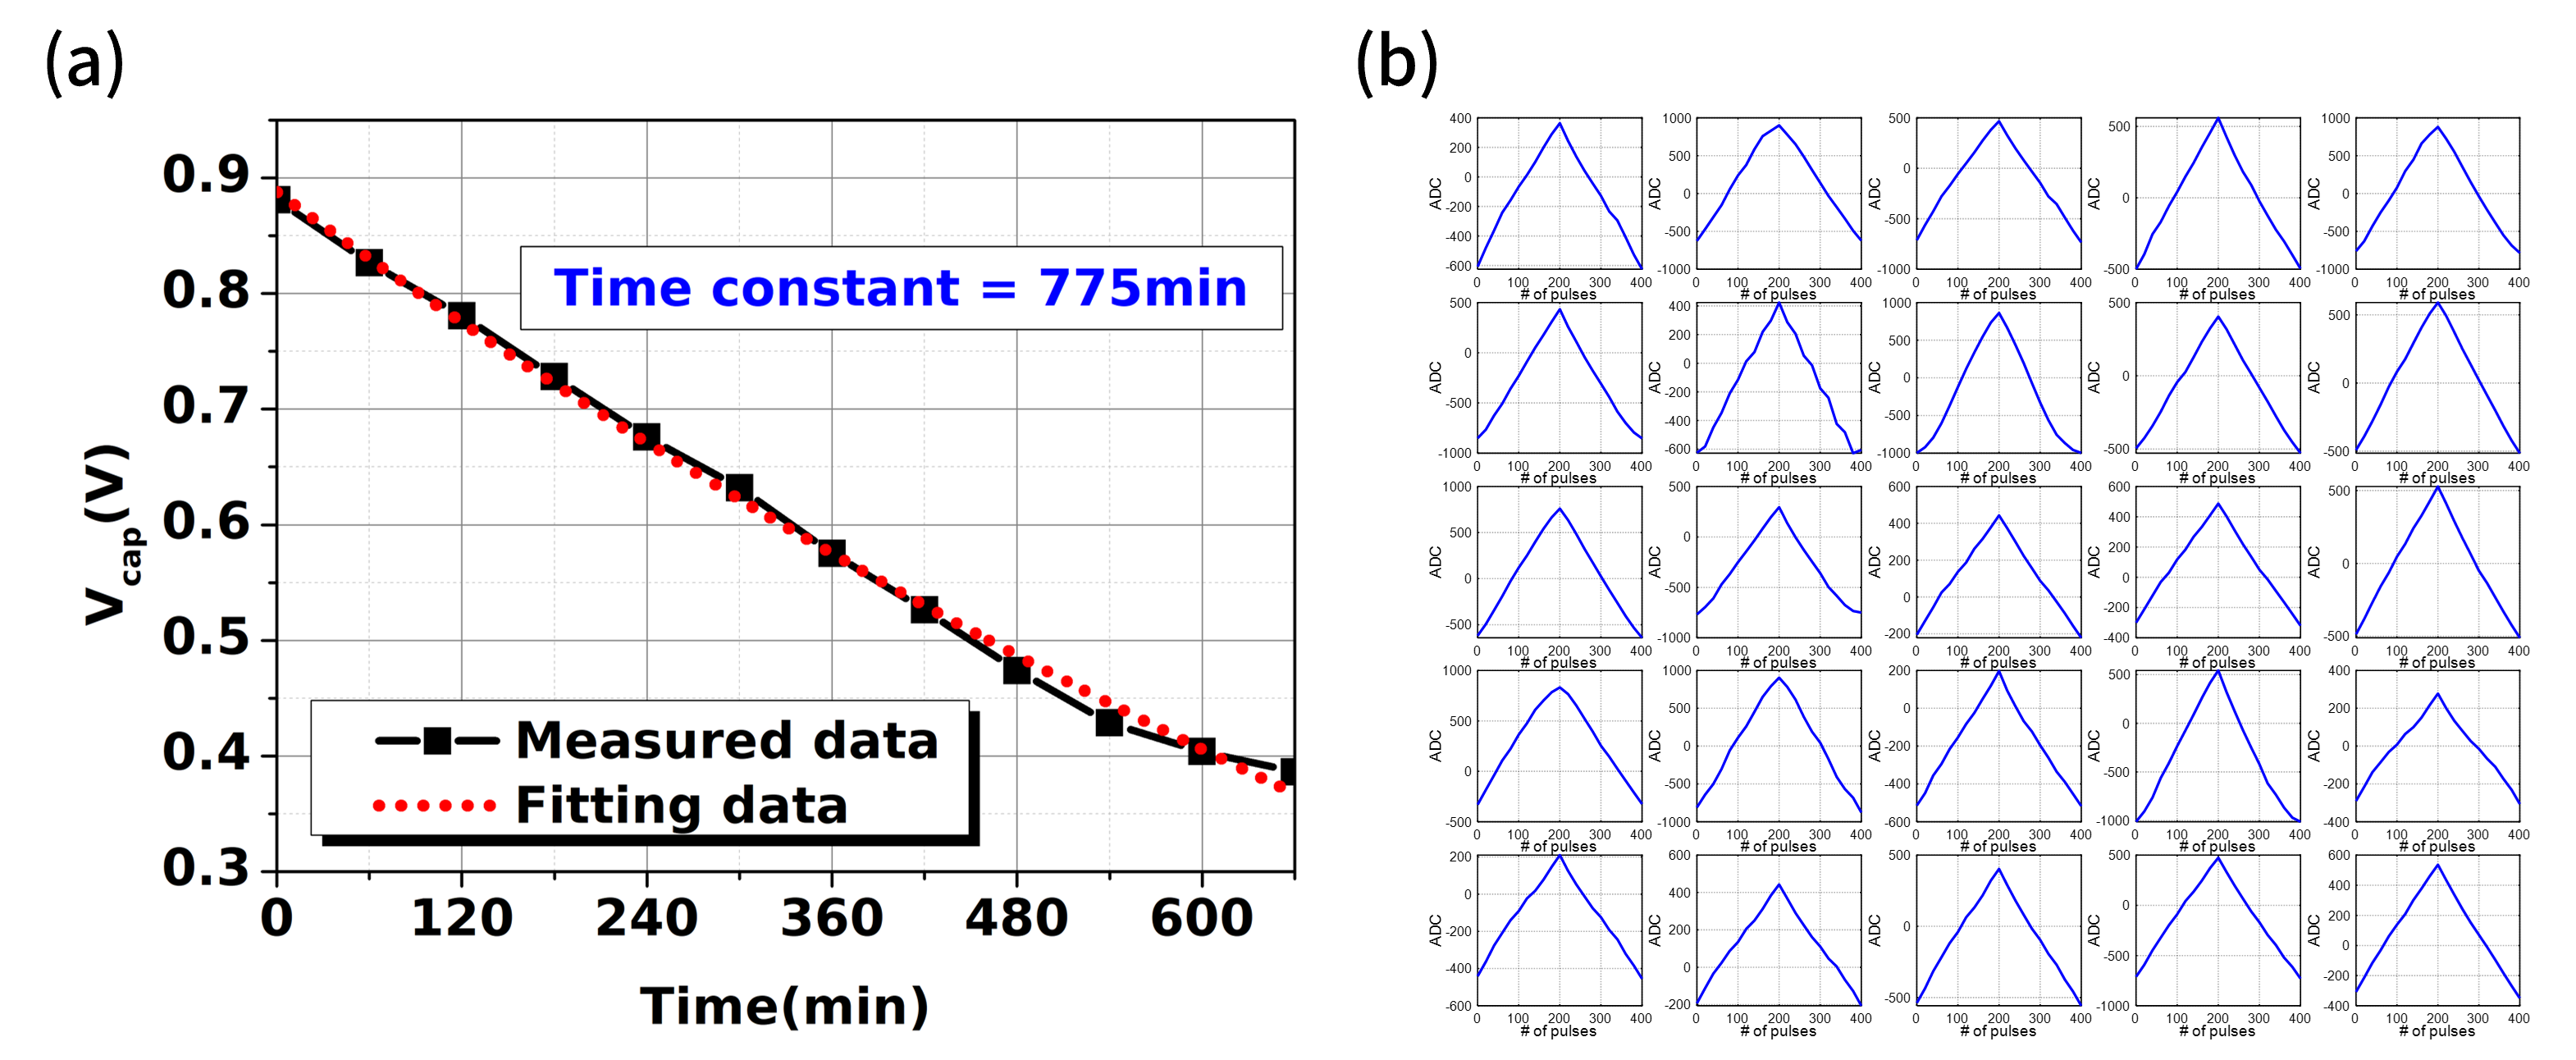
\includegraphics[width=0.98\textwidth]{sup_fig1.png}
  \caption{\textbf{Electrical Characteristics of the 6T1C Devices.}
  (a) Retention characteristics of the 6T1C device, demonstrating stable data retention. (b) Weight update characteristics of 25 cells in the fabricated 5x5 crossbar array. }
  \label{sup_fig1}
\end{figure}
\FloatBarrier

\SIEndSection

\section{Hardware setup and measurement platform}
\label{sec:S2}
%====================================================
\begin{figure}[!htbp]
  \centering
  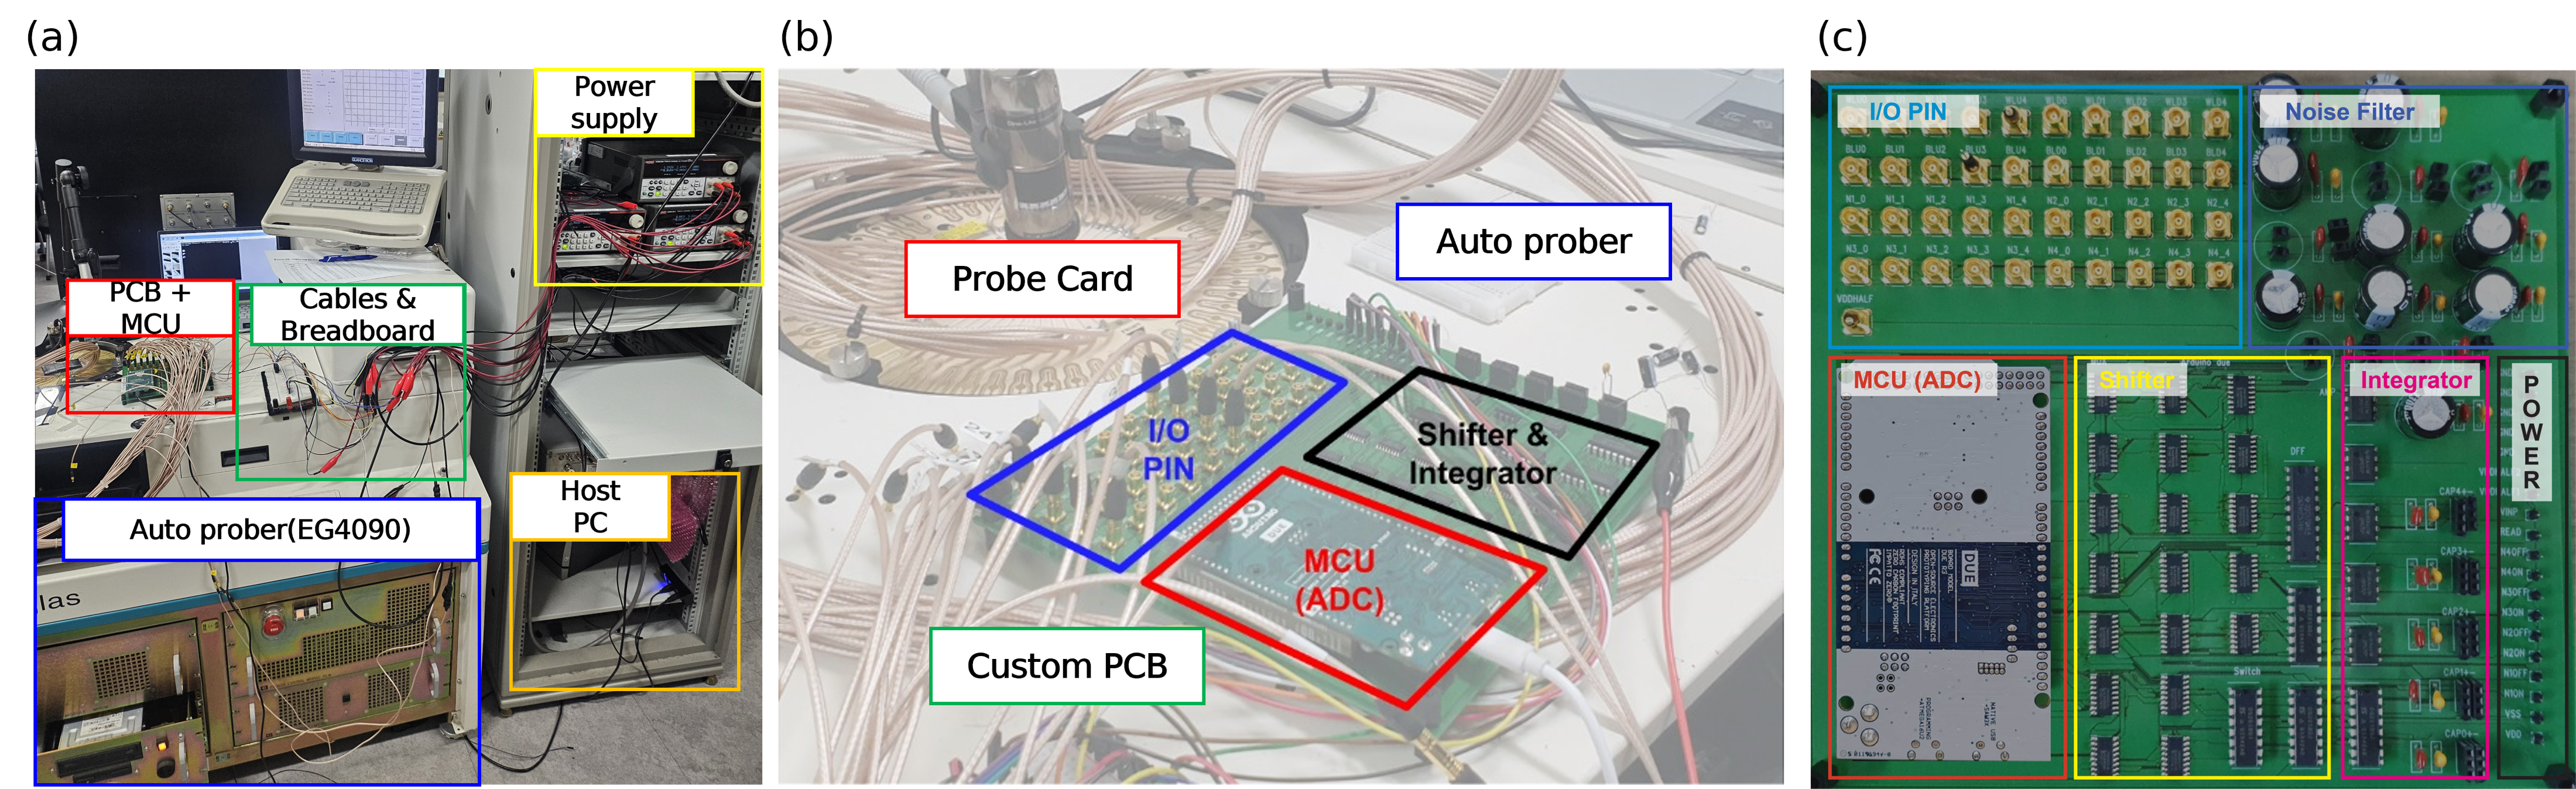
\includegraphics[width=0.98\textwidth]{sup_fig2.png}
  \caption{\textbf{}
(a) Overview of the measurement and hardware setup, including the auto-prober (Eg4090) with an 8-inch wafer loaded and a mounted probe card, a custom PCB connected to the probe card, a DC power supply for biasing, and associated cables and breadboards for signal routing and distribution. (b) Enlarged view of the probe card and custom PCB within the overall setup. (c) Photograph of the custom PCB used to apply update and read pulses to the synaptic devices, comprising multiplexers, analog switches, D flip-flops, operational amplifiers, and integration capacitors; measurement and hardware demonstration sequences are programmed via the MCU, with generated pulses delivered through I/O pins to the wafer. }
  \label{sup_fig2}
\end{figure}
\FloatBarrier

\SIEndSection
%====================================================
\section[Hardware rank-1 regression: core and auxiliary trajectories]
{Hardware rank-1 regression: core and auxiliary trajectories}
\label{sec:si_hardware_regression}
%====================================================

\noindent
This section reports the hardware-in-the-loop rank-1 regression experiment used to examine the transfer-period dependence of the core and auxiliary trajectories of LR-TT on the 6T1C array. The core matrix $C$ was maintained in the MCU loop, whereas the auxiliary factors $A\in\mathbb{R}^{1\times3}$ and $B\in\mathbb{R}^{3\times1}$ were programmed and read from the 6T1C sub-arrays. The auxiliary product $BA$ was reconstructed from the measured $A$ and $B$ states at the end of each accumulation window. Four transfer periods (TP $=1,4,10,20$) were compared under the same $1{,}000$-iteration budget. Supplementary Figs.~\ref{fig:si_hardware_regression_aux} and~\ref{fig:si_hardware_regression_core} summarize the resulting auxiliary and core trajectories, respectively.

\noindent\textbf{Auxiliary-array accumulation and trajectory stability.}
Supplementary Fig.~\ref{fig:si_hardware_regression_aux} shows that increasing TP(Transfer Period) retains a larger auxiliary state between transfers. This trend is beneficial only up to an intermediate TP. TP $=20$ reaches the target range rapidly at early stages, but it also shows larger late-stage fluctuations in the auxiliary factors and a less settled core trajectory than TP $\le 10$. Accordingly, TP defines a speed--stability trade-off: longer accumulation produces a larger core update at transfer, whereas excessively large TP leads to larger late-stage fluctuations in the auxiliary factors.

\noindent\textbf{Core-array convergence and TP dependence.}
As shown in Supplementary Fig.~\ref{fig:si_hardware_regression_core}, all TP settings drive $C$ toward $T$, including the negative second column of the target, confirming stable bidirectional operation in the hardware loop. The final residuals $\|T-C\|_F$ are $0.102$, $0.087$, $0.073$, and $0.143$ for TP $=1,4,10,20$, respectively, with corresponding element-wise MAE values of $0.030$, $0.025$, $0.023$, and $0.037$. Among the tested conditions, TP $=10$ gives the smallest final error. The same figure also shows that increasing TP makes the core evolution progressively more staircased, consistent with a larger accumulated correction being consolidated at each transfer.

\begin{figure}[!htbp]
  \centering
  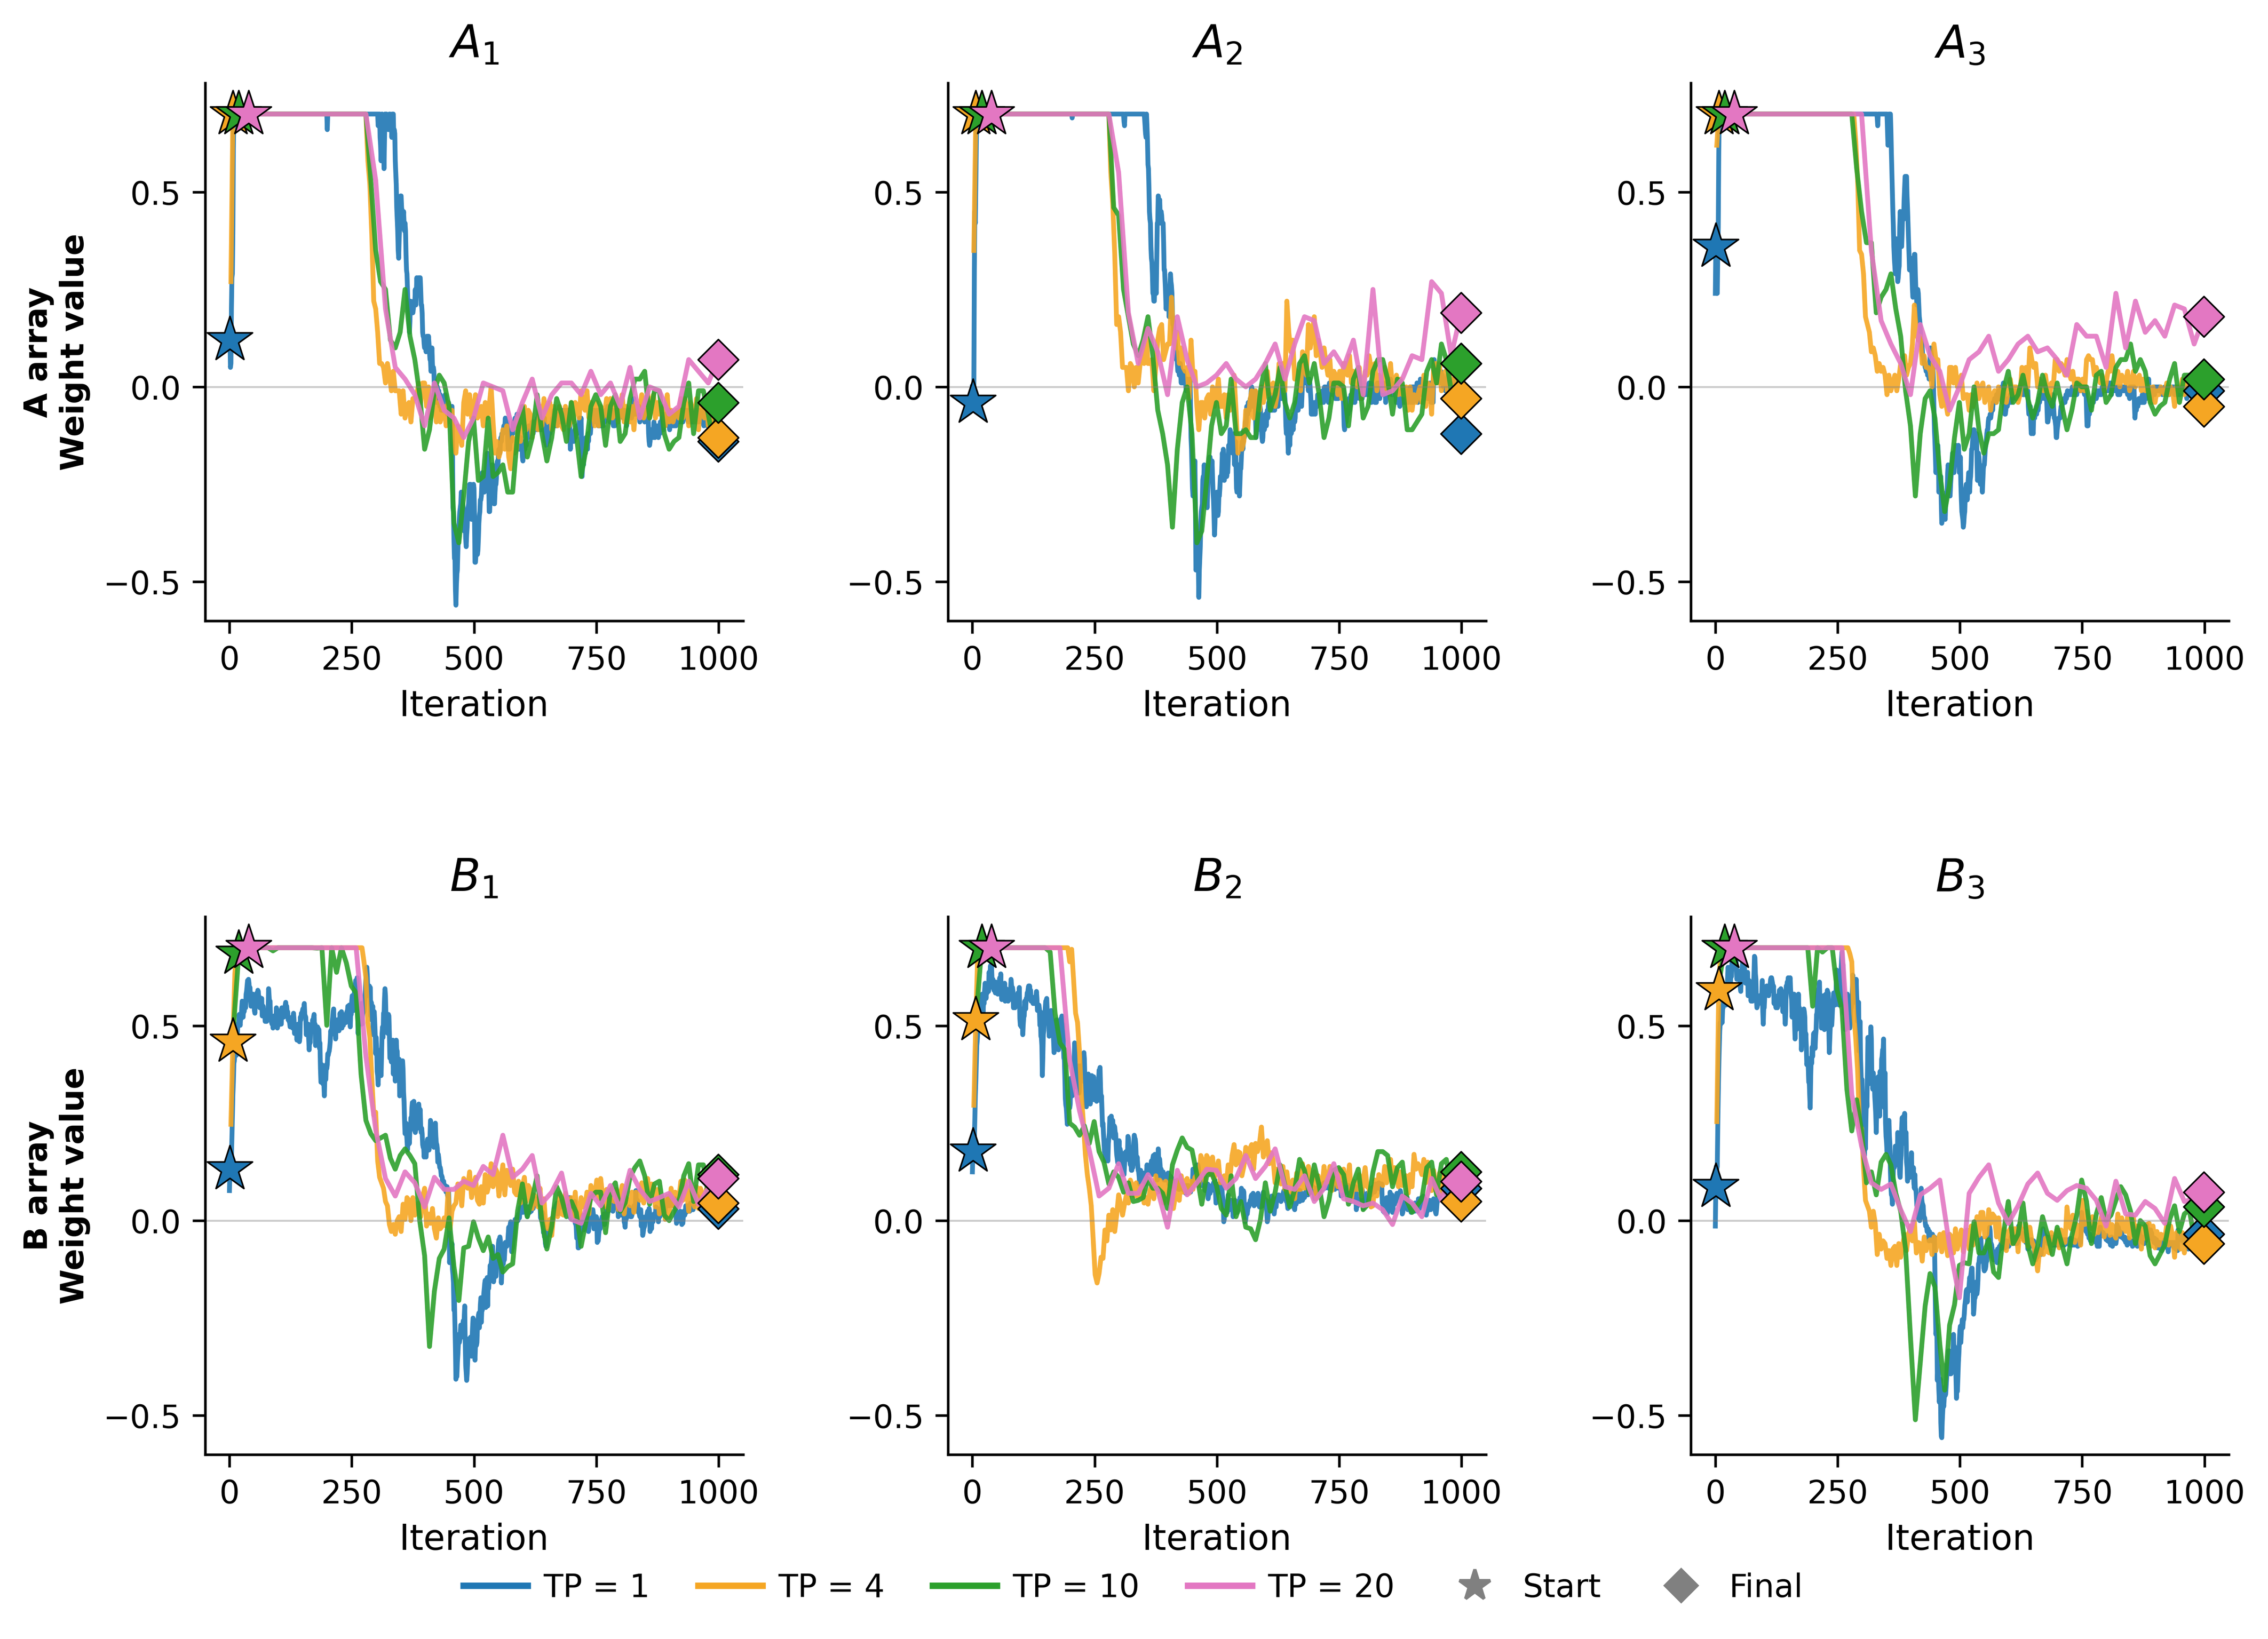
\includegraphics[width=0.98\textwidth]{sup_fig3a.png}
  \caption{\textbf{Hardware rank-1 regression: auxiliary trajectories under different transfer periods.}
  Training-step evolution of the measured auxiliary factors $A$ and $B$ for TP $=1,4,10,20$.
  Larger TP retains a larger accumulated auxiliary state between successive transfers and leads to more persistent late-stage fluctuations.}
  \label{fig:si_hardware_regression_aux}
\end{figure}
\FloatBarrier

\begin{figure}[t]
  \centering
  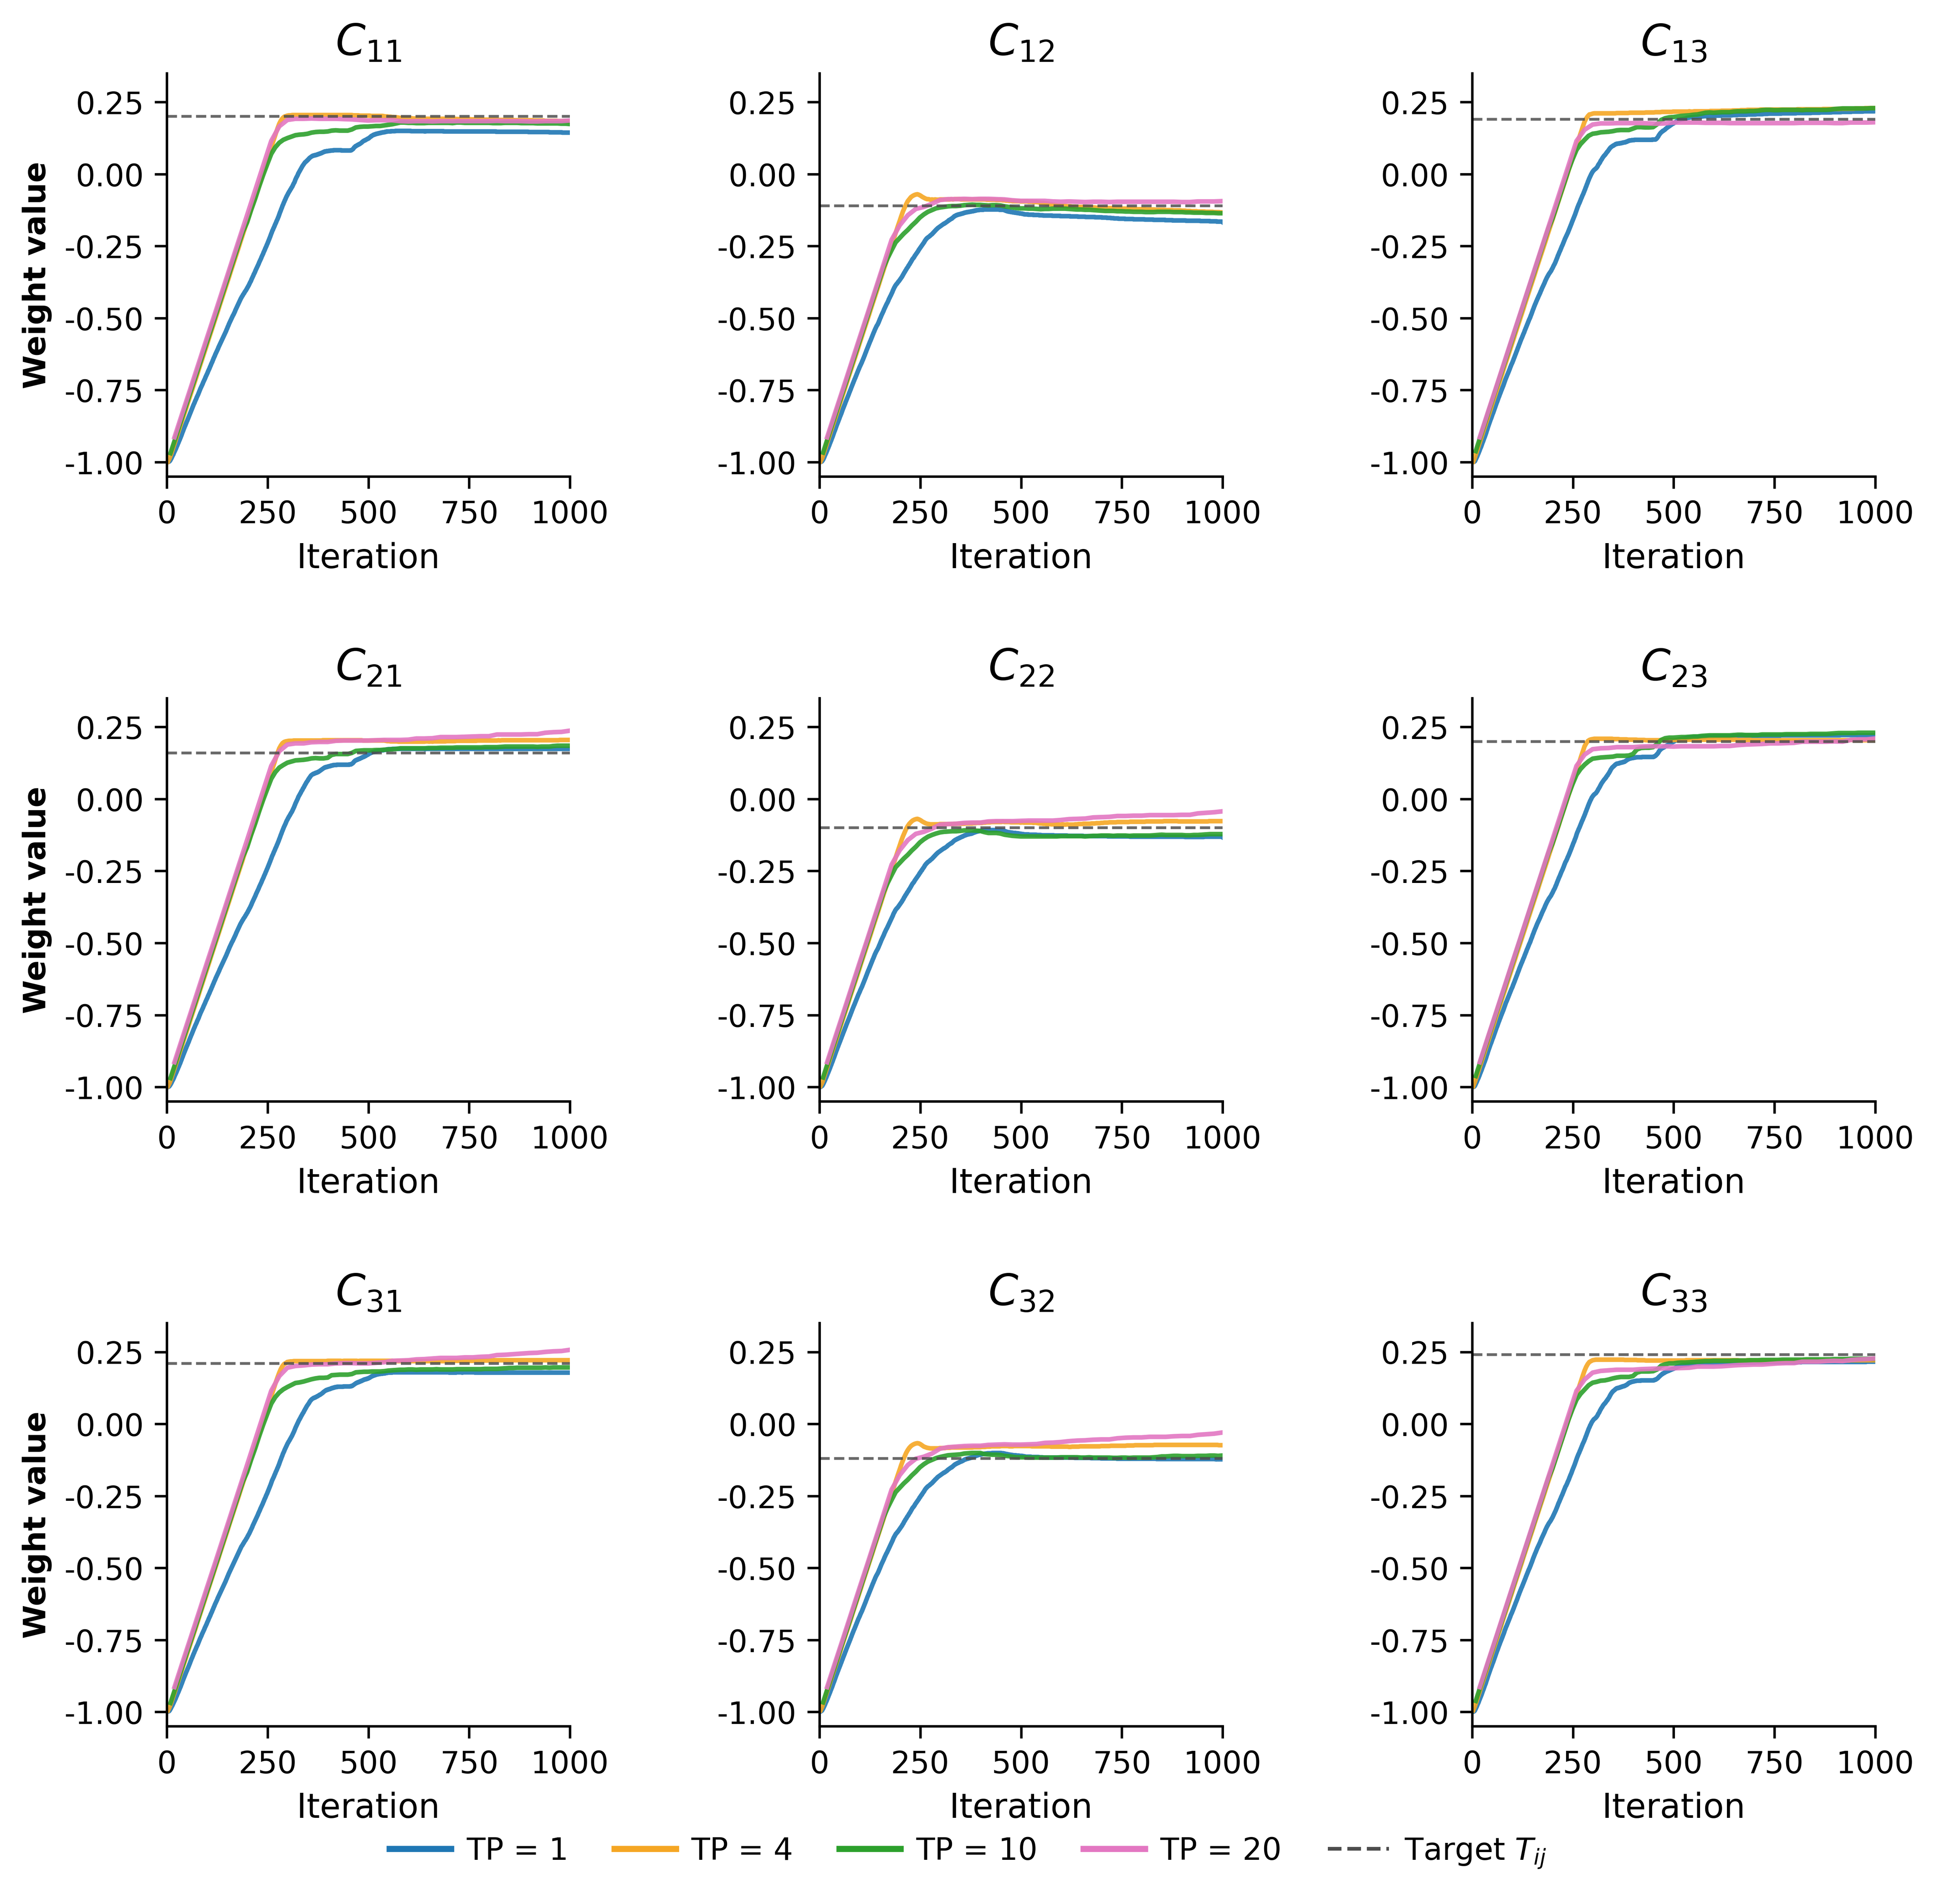
\includegraphics[width=0.98\textwidth]{sup_fig3b.png}
  \caption{\textbf{Hardware rank-1 regression: core trajectories under different transfer periods.}
  Element-wise evolution of the core matrix $C$ for TP $=1,4,10,20$; dashed lines indicate the target entries of $T$.
  All TP settings drive the core trajectory toward the target, while larger TP makes the evolution more staircased.}
  \label{fig:si_hardware_regression_core}
\end{figure}
\FloatBarrier

\SIEndSection


\section[Training trajectory under C-tile and A/B-tile asymmetry]{Training trajectory under $C$-tile and $A/B$-tile asymmetry} \label{sec:S4}

\noindent
This section examines the sensitivity of the LR-TT optimization trajectory to device nonlinearity. Using the same \(9\times9\) simulated regression setting as in main-text Fig.~4d,e, the asymmetry factor was varied while all other conditions were kept at the values optimized for the baseline AF calibrated to the 6T1C hardware: rank \(r=1\), transfer period \(\tau=10\), one-hot transfer, a SoftBounds core-tile device model, and ideal I/O (\texttt{is\_perfect=True}). The PCA basis for each panel was fitted jointly over all trajectories within that panel.

\noindent
Supplementary Fig.~\ref{fig:si_asymmetry_trajectory}a shows the core-tile asymmetry dependence (\(\mathrm{AF}^{C}\in\{0,1,2,5\}\)) at fixed baseline auxiliary-tile AF, together with a direct-\(C\) SGD (FP32) reference. As \(\mathrm{AF}^{C}\) increases, the trajectory deviates progressively from the baseline path, with \(\mathrm{AF}^{C}=5\) showing the most significant degradation. The step-milestone markers further indicate that convergence slows as the asymmetry factor increases. 

\noindent
Supplementary Fig.~\ref{fig:si_asymmetry_trajectory}b shows the corresponding auxiliary-tile asymmetry dependence (\(\mathrm{AF}^{A,B}\in\{0,1,2,5\}\)) at fixed baseline core-tile AF. Similarly, increasing auxiliary-tile nonlinearity degrades the trajectory, with \(\mathrm{AF}^{A,B}=5\) also showing substantial deviation and slower convergence.

\noindent
In both cases, hyperparameters were not re-tuned for each AF setting, so the observed degradation reflects the direct effect of device nonlinearity on an otherwise fixed optimization configuration \cite{lee2022tikitaka_asymmetry,wu2024exact}. The detailed definition of AF (Asymmetric Factor) is explained in  Eq.~\eqref{eq:S8_effective_slope} and ~\eqref{eq:S8_af_ratio}. Full experimental parameters are provided in Supplementary Section~\ref{sec:S8}.

\begin{figure}[!htbp]
  \centering
  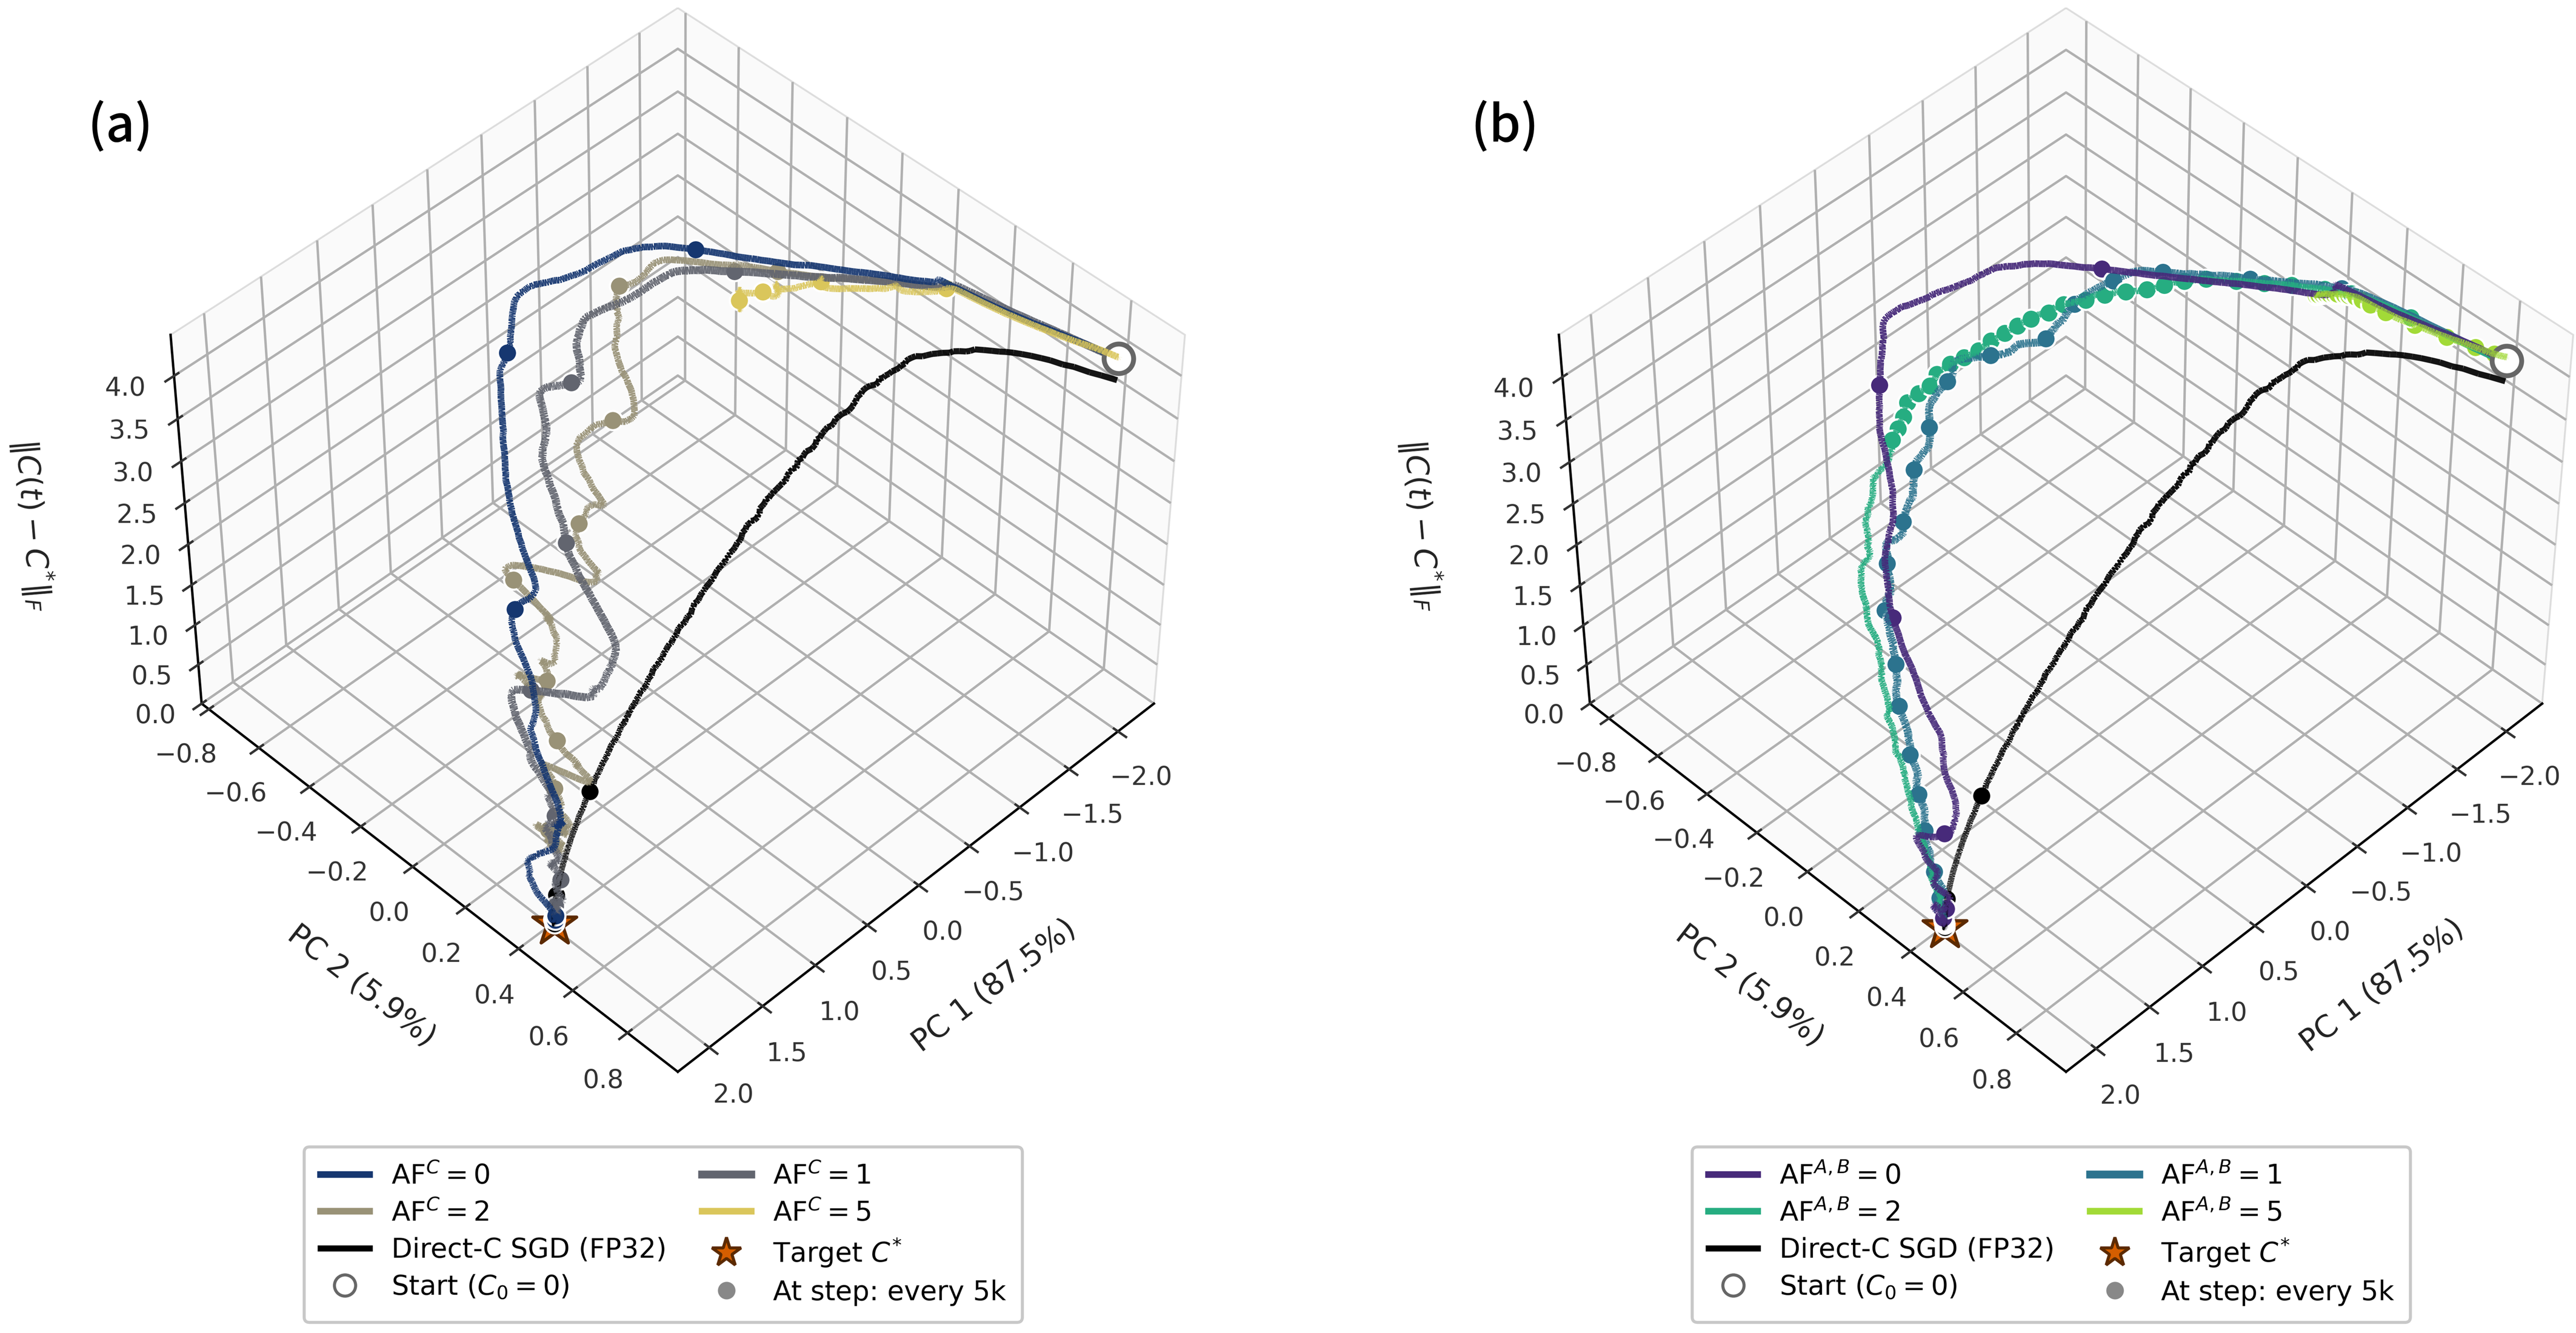
\includegraphics[width=0.98\textwidth]{sup_fig4.png}
  \caption{\textbf{Training trajectory under core-tile and auxiliary-tile asymmetry.}
  (a) Dependence on the core-tile asymmetry factor, $\mathrm{AF}^{C}\in\{0,1,2,5\}$, at fixed baseline auxiliary-tile asymmetry, together with a direct-$C$ SGD (FP32) reference.
  (b) Dependence on the auxiliary-tile asymmetry factor, $\mathrm{AF}^{A,B}\in\{0,1,2,5\}$, at fixed baseline core-tile asymmetry, with the same SGD (FP32) reference.
  In both panels, the PCA basis is fitted jointly over all trajectories within the panel, the $z$-axis represents the training loss, and diamond markers indicate convergence speed.}
  \label{fig:si_asymmetry_trajectory}
\end{figure}
\SIEndSection


\section[Post-transfer reset/retention and auxiliary forward path during training]{Post-transfer reset/retention and auxiliary forward path during training}
\label{sec:S5}
%====================================================

\noindent
This section describes three implementation details used to interpret the reset comparison in Supplementary Fig.~\ref{fig:si_reset_aux_path}: the auxiliary forward path, the post-transfer reset/retention rule, and the effective-rank measure of the cumulative core-array update.

\noindent\textbf{Auxiliary forward path.}
For a mapped layer \(\ell\), LR-TT maintains one core array and two auxiliary arrays,
\begin{equation}
C_{\ell,t}\in\mathbb{R}^{d_{\mathrm{out},\ell}\times d_{\mathrm{in},\ell}},
\qquad
A_{\ell,t}\in\mathbb{R}^{r_\ell\times d_{\mathrm{in},\ell}},
\qquad
B_{\ell,t}\in\mathbb{R}^{d_{\mathrm{out},\ell}\times r_\ell}.
\label{eq:S4_state_definition}
\end{equation}
The auxiliary arrays form a low-rank product \(B_{\ell,t}A_{\ell,t}\), whereas the core array \(C_{\ell,t}\) stores the core weight of the mapped layer. During training, the forward-path weight is written as
\begin{equation}
W_{\ell,t}
=
C_{\ell,t}
+
\gamma_\ell \alpha_\ell B_{\ell,t}A_{\ell,t},
\qquad
Y_{\ell,t}=W_{\ell,t}X_{\ell,t},
\label{eq:S4_aux_forward}
\end{equation}
where \(\alpha_\ell\) is the LoRA scaling coefficient and \(\gamma_\ell\) controls the contribution of the auxiliary state to the forward path \cite{gokmen2020tikitaka,hu2021lora}. When \(\gamma_\ell=0\), the forward computation is defined only by the core array \(C_{\ell,t}\), whereas \(\gamma_\ell>0\) allows the auxiliary product to contribute directly to the forward-path weight.

\noindent\textbf{Post-transfer reset/retention rule.}
At transfer steps, the accumulated auxiliary product is transferred to the core array,
\begin{equation}
C_{\ell,t+1}
=
C_{\ell,t}
+
\eta_{\mathrm{tr},\ell}B_{\ell,t}^{+}A_{\ell,t}^{+},
\label{eq:S4_core_transfer}
\end{equation}
where \(A_{\ell,t}^{+}\) and \(B_{\ell,t}^{+}\) denote the auxiliary states immediately before the post-transfer rule is applied, and \(\eta_{\mathrm{tr},\ell}\) is the transfer learning rate. Following the notation of the Eqs. (2), the \(A\) factor is retained after transfer,
\begin{equation}
A_{\ell,t+1}=A_{\ell,t}^{+},
\label{eq:S4_post_A}
\end{equation}
whereas the post-transfer rule is applied to the \(B\) factor:
\begin{equation}
\text{w/ reset:}
\qquad
B_{\ell,t+1}=B_{\ell}^{(0)},
\label{eq:S4_reset_rule}
\end{equation}
\begin{equation}
\text{w/o reset:}
\qquad
B_{\ell,t+1}=B_{\ell,t}^{+}.
\label{eq:S4_nonreset_rule}
\end{equation}
Thus, the compared conditions differ only in whether the transferred \(B\)-factor state is reset or retained after each \(BA\rightarrow C\) transfer. Because \(\gamma=0\), this comparison does not alter the forward path directly; instead, it isolates how the post-transfer auxiliary-state rule changes the initial condition of the next accumulation window.

\noindent\textbf{Effective rank of the cumulative core-array update.}
To quantify the dimensionality of the cumulative update transferred to the core array, we measure
\begin{equation}
\Delta C_t = C_t-C_0.
\label{eq:S4_deltaC}
\end{equation}
The entropy effective rank is then computed from the singular values \(\{\sigma_i\}\) of \(\Delta C_t\):
\begin{equation}
p_i=\frac{\sigma_i}{\sum_j\sigma_j},
\qquad
\erank(\Delta C_t)
=
\exp\!\left(
-\sum_i p_i\ln p_i
\right).
\label{eq:S4_erank}
\end{equation}
This metric is scale-invariant and measures how evenly the transferred update energy is distributed across singular directions, rather than how large the update is in norm \cite{roy2007effective}. In the MNIST comparison, \(\erank(\Delta C_t)\) is evaluated for the first mapped layer only.

\noindent
Supplementary Fig.~\ref{fig:si_reset_aux_path} shows that the w/o reset mode yields higher MNIST accuracy in most rank--transfer-period cells, whereas the w/ reset mode often produces a larger \(\erank(\Delta C)\), indicating that task performance is not determined by the dimensionality of the cumulative update transferred to the core array alone. We interpret this as a stability--diversity trade-off: resetting the post-transfer \(B\)-factor state broadens the subspace populated by successive transferred updates, but in the \(\gamma=0\) regime it also weakens the continuity of auxiliary-state accumulation across transfer windows, so retaining the transferred \(B\)-factor state more often yields higher MNIST accuracy even when the resulting \(\erank(\Delta C)\) is lower.

\begin{figure}[!t]
  \centering
  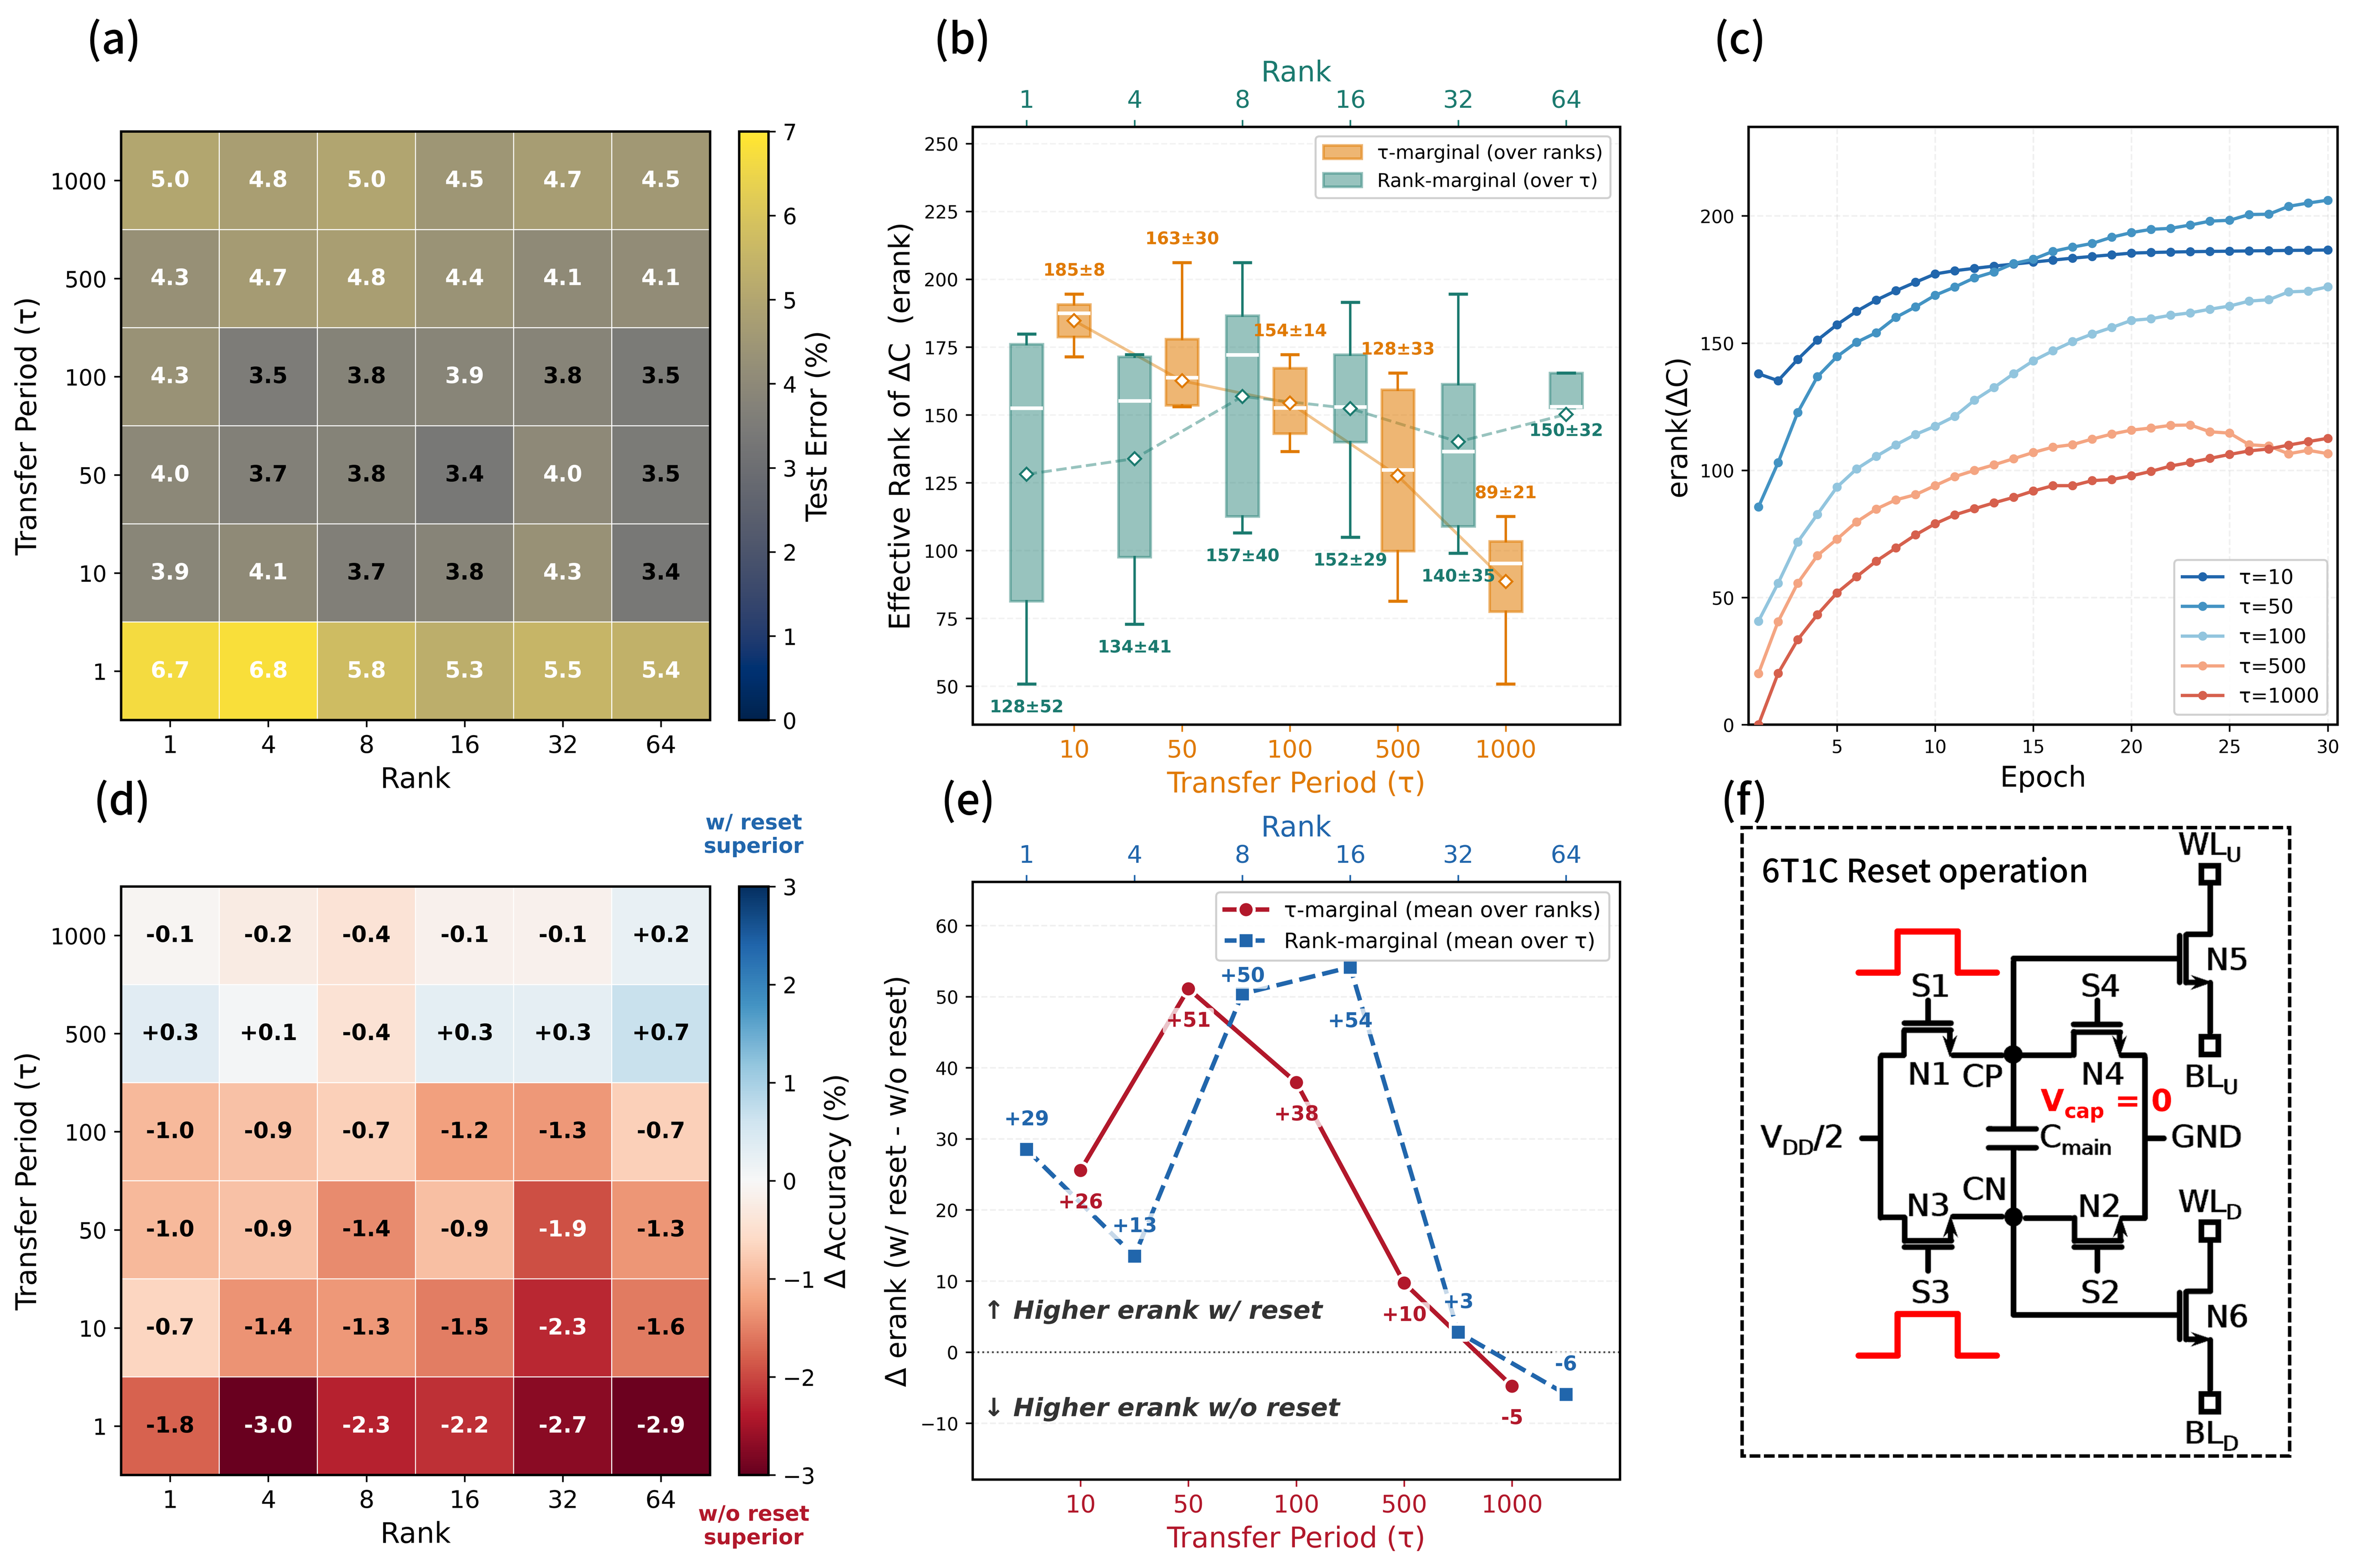
\includegraphics[width=0.98\textwidth]{sup_fig5.png}
  \caption{\textbf{MNIST comparison of LR-TT training with and without post-transfer reset.}
  (a) Test error of the with-reset mode as a function of LoRA rank and transfer period $\tau$.
  (b) Effective rank of the cumulative core-array update, $\erank(\Delta C)$, for the with-reset mode, summarized by $\tau$-marginal and rank-marginal distributions. (c) Epoch-wise evolution of $\erank(\Delta C)$ for the without-reset mode at rank $r=8$.
  (d) Paired accuracy difference, $\Delta\mathrm{Acc}=\mathrm{Acc}_{\mathrm{reset}}-\mathrm{Acc}_{\mathrm{nonreset}}$, at matched rank and $\tau$; negative values indicate that the without-reset mode gives higher accuracy.
  (e) Paired effective-rank difference, $\Delta\erank=\erank_{\mathrm{reset}}-\erank_{\mathrm{nonreset}}$, summarized along the $\tau$ and rank axes. 
  (f) Hard-reset operation of the 6T1C synaptic device. In the 6T1C, the weight is encoded in the capacitor voltage (Vcap), which is inherently bounded within a range of -VDD/2 to VDD/2. Accordingly, Vcap = 0 corresponds to a zero-weight state. As illustrated, simultaneous pulses applied to S1 and S3 set both the CP and CN nodes to VDD/2, enabling a straightforward and reliable reset to the zero-weight condition.}
  \label{fig:si_reset_aux_path}
\end{figure}

% \begin{table}[!htbp]
% \centering
% \caption{\textbf{Exploratory LR-TT extensions on BERT-base SQuAD.}
% As a preliminary feasibility check, we tested two variants that extend the
% main-text default by enabling auxiliary forward-path participation
% ($\gamma_\ell>0$) (See definition in Eq.~\eqref{eq:S4_aux_forward})  together with the partial post-transfer reset rule
% (``w/'' reset; Supplementary Eq.~\eqref{eq:S4_reset_rule}, equivalent to the
% \texttt{hybrid} reinitialization mode in the implementation), evaluated with
% rank-wise stochastic pulse transfer (RW) and ideal analytic transfer (Id).
% These runs used limited Optuna searches with no dedicated hyperparameter
% tuning at this regime; the F1 values below should be read as an indication
% that these extensions also train successfully on this task rather than as
% optimized results. All other settings follow the configuration used for these runs (rank $r=32$, QKVO mapping, constant-step-ideal auxiliary-tile device, $|w|_{\max}^{A,B}=1.0$ without multilevel updates).}
% \label{tab:S5_lrtt_variants}
% \small
% \renewcommand{\arraystretch}{1.10}
% \setlength{\tabcolsep}{4.0pt}
% \begin{tabular}{c c c c c c r r}
% \toprule
% \rowcolor{HeadGray}
% \textbf{$\gamma_\ell$} & \textbf{Reset} & \textbf{Transfer} & \textbf{$r$} &
% \textbf{$|w|_{\max}^{A,B}$} & \textbf{C bit} &
% \textbf{Optuna trials} & \textbf{Best F1} \\
% \midrule
% $>0$ & w/ & RW & 32 & 1.0 & 10 & 94 & 85.85 \\
% $>0$ & w/ & Id & 32 & 1.0 & 10 & 44 & 87.21 \\
% \bottomrule
% \end{tabular}
% \end{table}

\SIEndSection

%====================================================
\section{Supplementary training analysis for BERT-base fine-tuning}
\label{sec:S6}
%====================================================

\noindent
This section presents additional diagnostics and ablations that complement the BERT-base fine-tuning results in Fig. 5 of the main manuscript.


  \begin{figure}[!htbp]                                                                                        
    \centering                                                                                              
    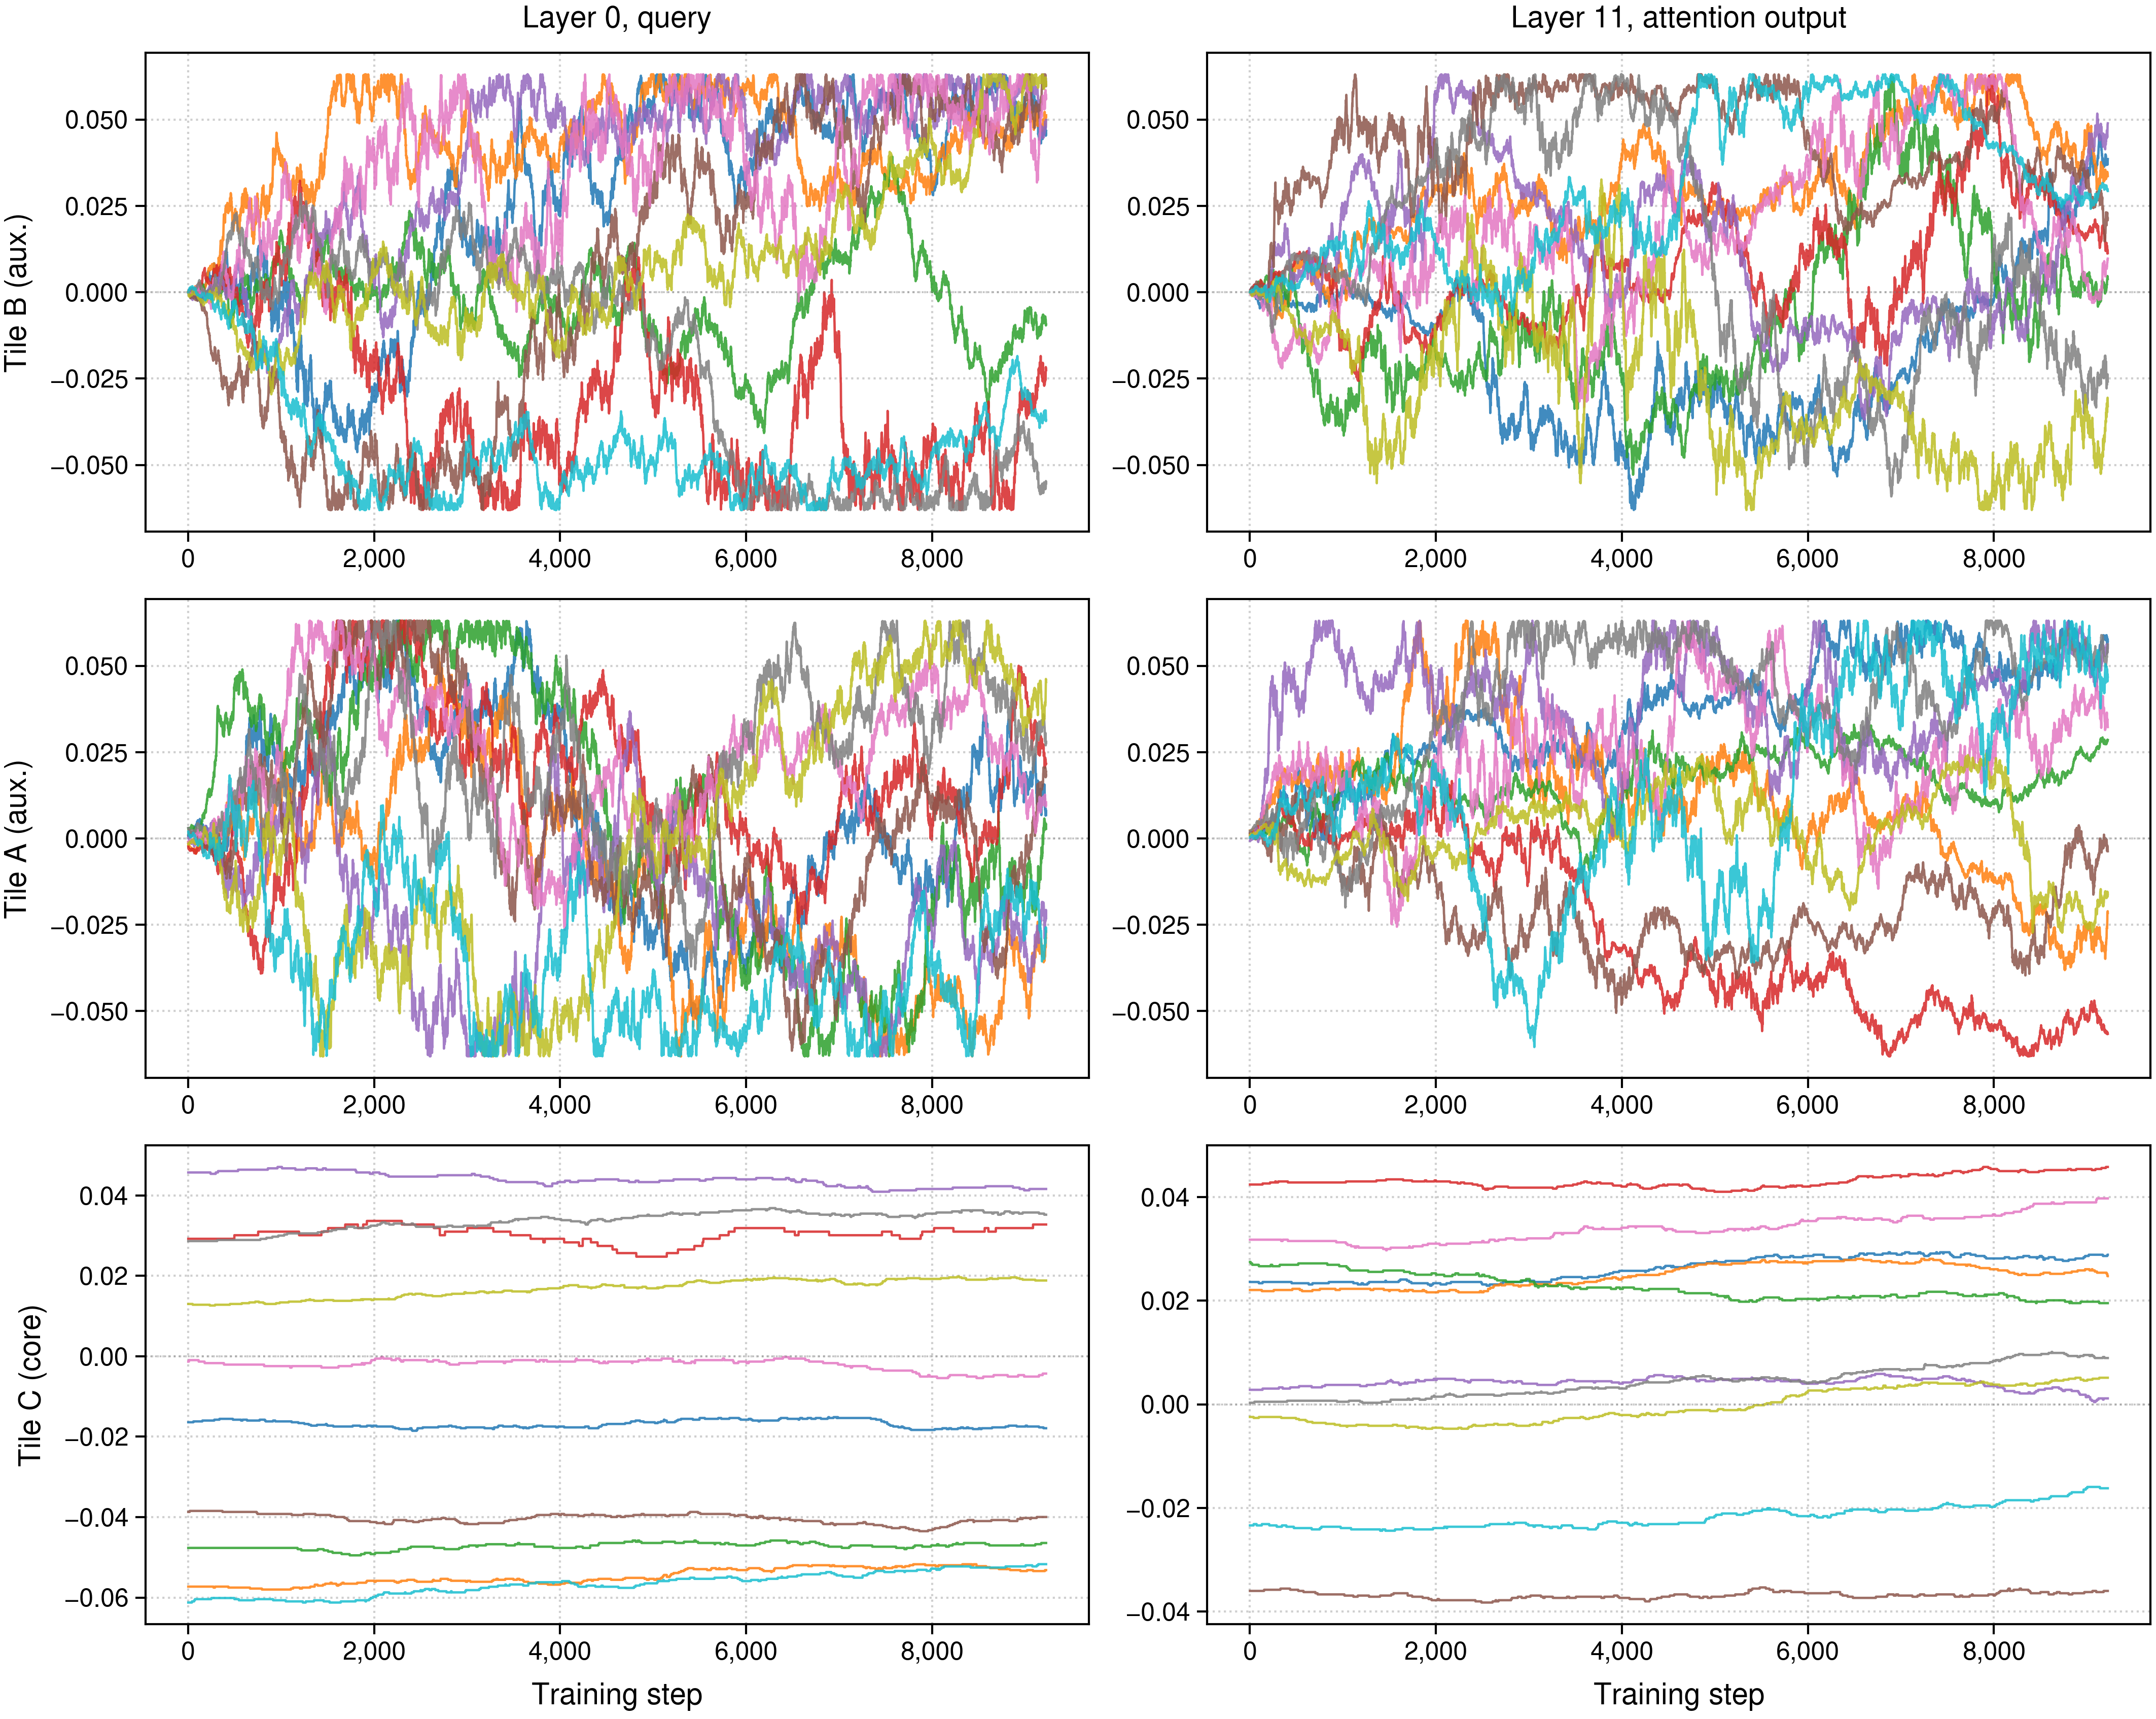
\includegraphics[width=0.98\textwidth]{sup_fig6_1.png}                                                  
    \caption{\textbf{Per-cell weight dynamics of the auxiliary ($A$, $B$)                                   
    and core ($C$) tiles during LR-TT fine-tuning of BERT-base on                                           
    SQuAD~v1.1 (rank $r=32$, rank-wise stochastic transfer).}                                                            
    The \emph{left column} shows the Layer~0 query projection and the                                       
    \emph{right column} shows the Layer~11 attention-output projection.                                     
    From top to bottom, the rows plot the trajectories of 10 randomly                                       
    sampled cells from tile~$B$ (auxiliary), tile~$A$ (auxiliary), and                                      
    tile~$C$ (core), respectively. The auxiliary tiles (top and middle)                                     
    exhibit random-walk-like excursions bounded by the device range                                         
    $|w|_{\max}^{A,B}\!\approx\!6.3\times10^{-2}$, reflecting the auxiliary low-rank
    accumulation that is periodically consolidated by rank-wise stochastic transfer, whereas                                    
    the core tile (bottom) evolves on a much slower timescale, with each cell holding a nearly constant level around its programmed pretrained value that drifts only marginally as transfers accumulate. Conditions: analog $A$/$B$ with a 10-bit constant-step-ideal response                                                                            
    ($\Delta w_{\min}\!=\!1.23\!\times\!10^{-4}$), 10-bit constant-step                                     
    $C$ ($\Delta w_{\min}\!=\!1.95\!\times\!10^{-3}$), transfer learning rate $7.87\times10^{-4}$ (constant), auxiliary fast-tile learning-rate scale $0.68$, peak learning rate $1.11\times10^{-3}$.}                                                           
    \label{sub_fig6_1}                                                                                      
  \end{figure}     

    \begin{figure}[t]                                                                                         
    \centering                                                                                              
    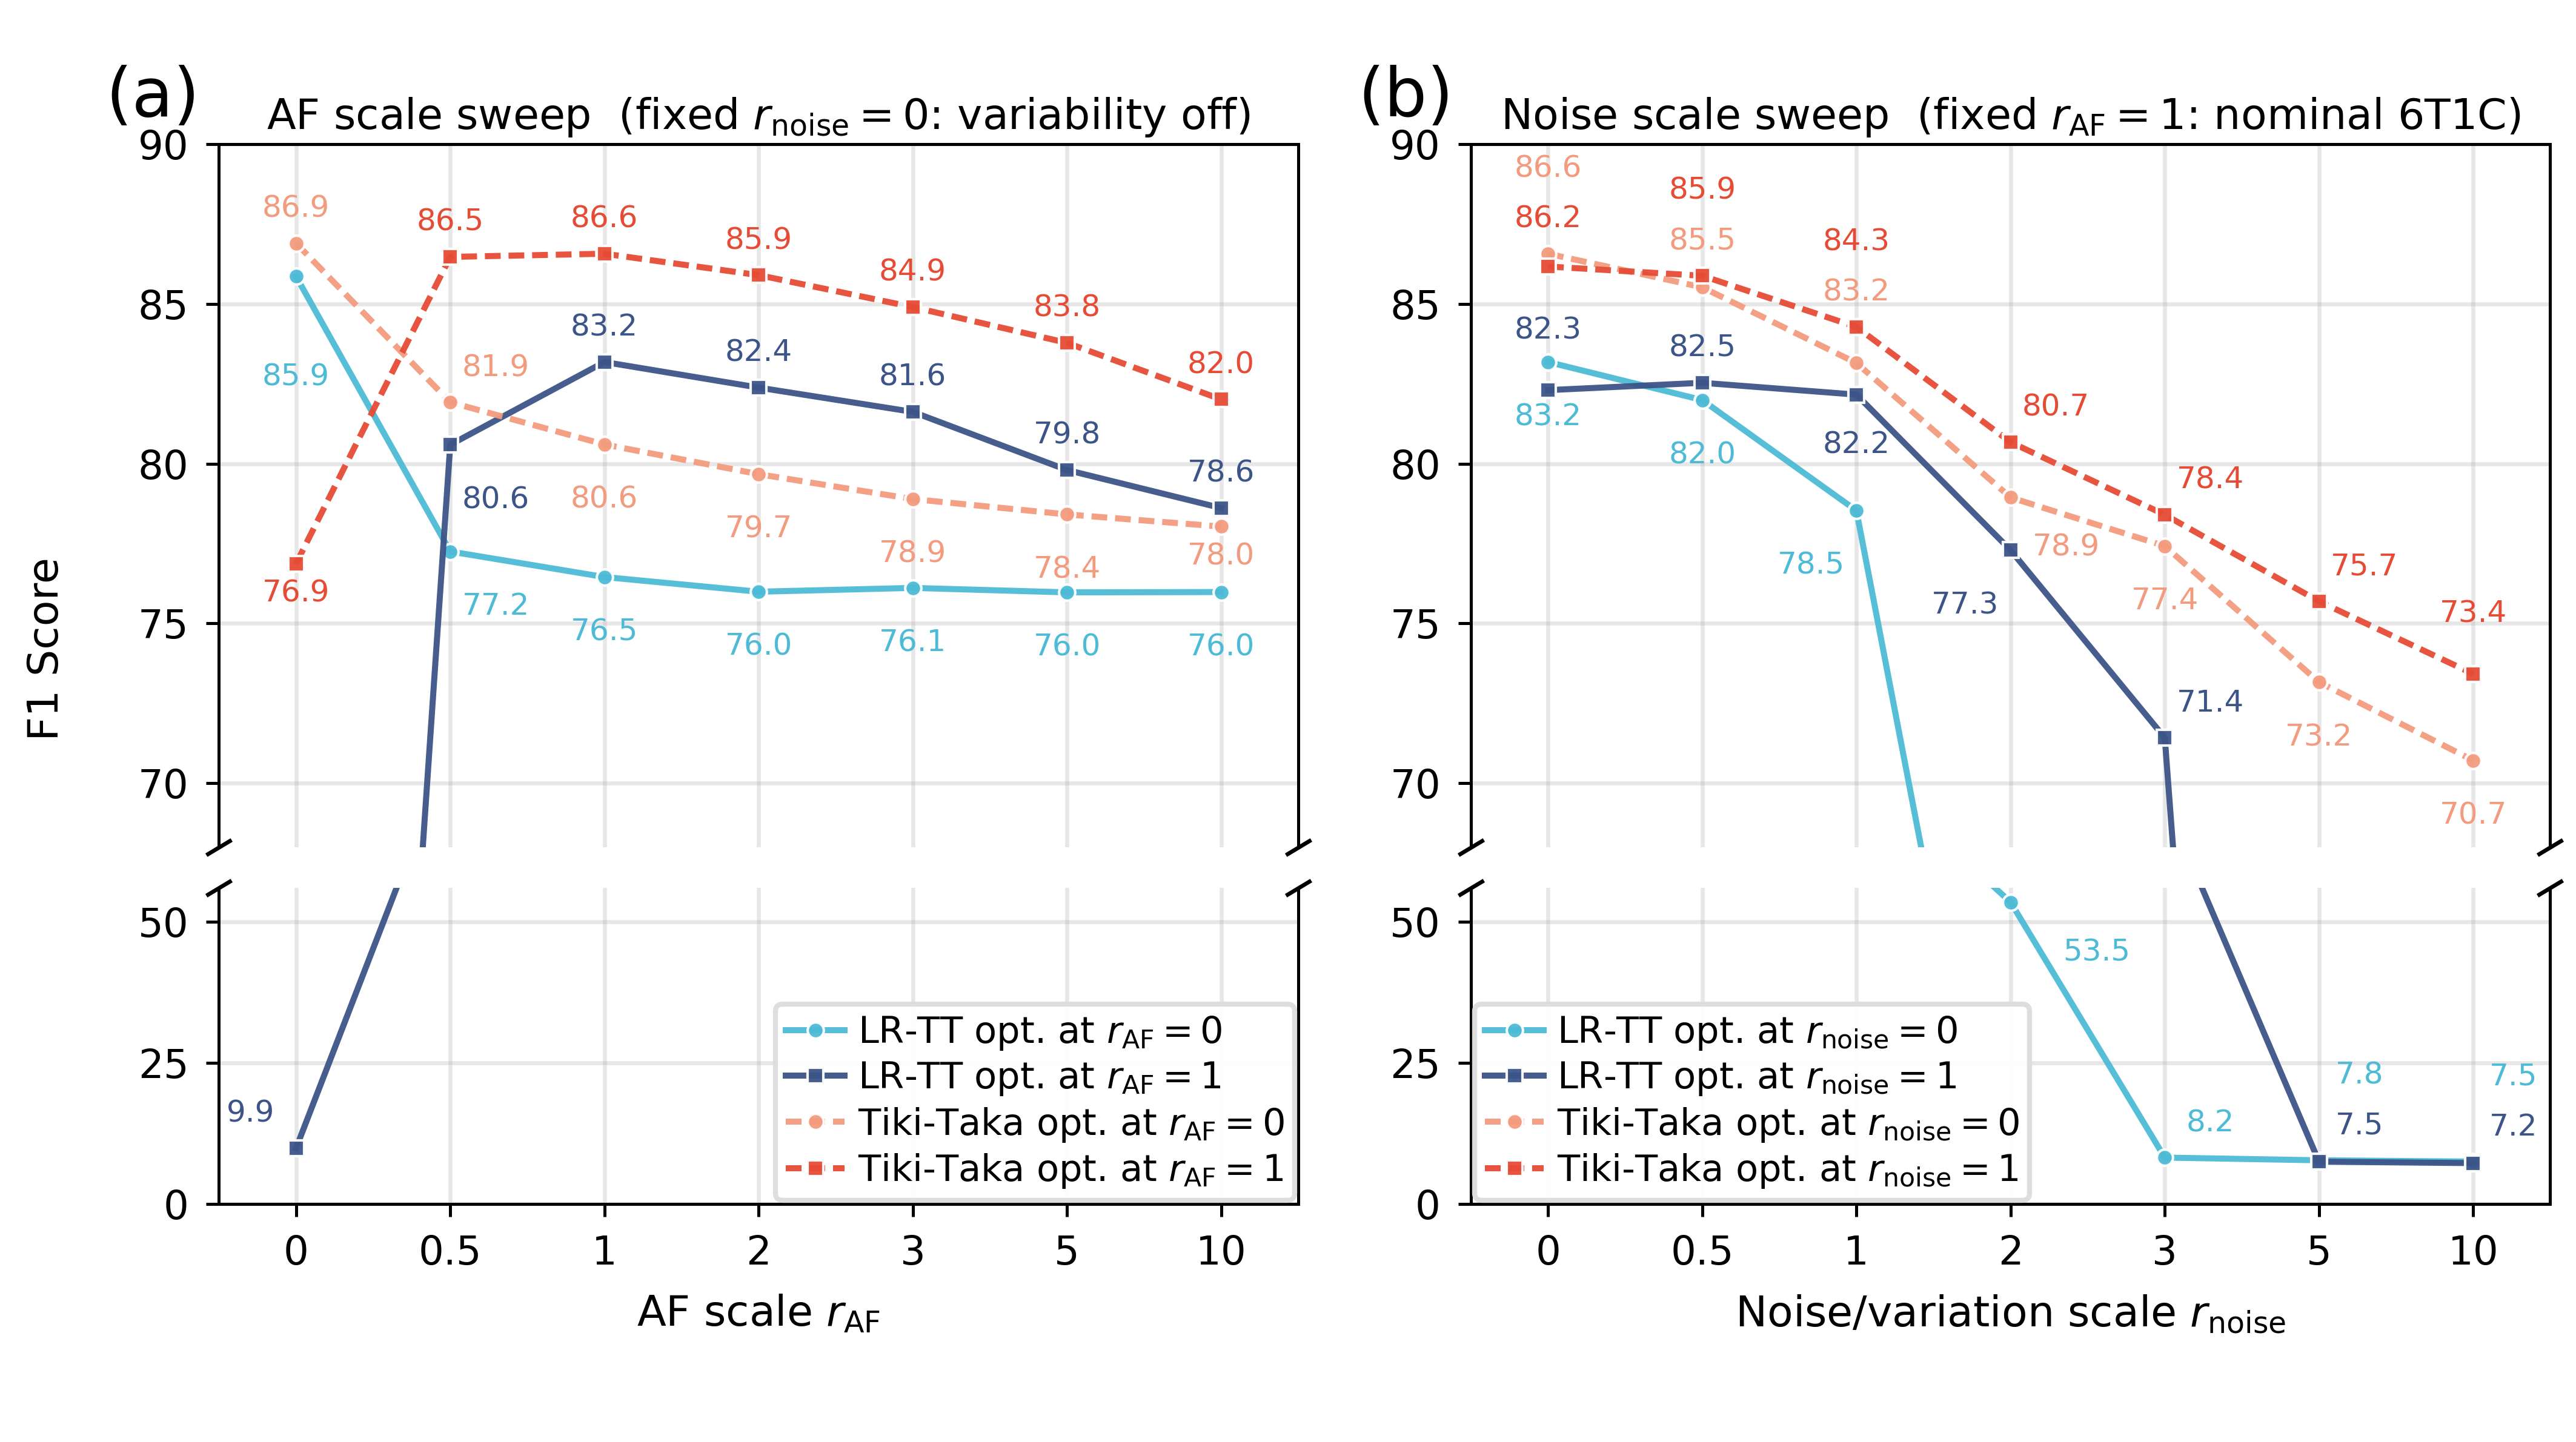
\includegraphics[width=0.98\textwidth]{sup_fig6_2.png}                                                  
    \caption{\textbf{Full sensitivity analysis of LR-TT to auxiliary-device asymmetry and noise/variation.}
    Sensitivity analysis underlying the three conditions summarized in Fig.~6c, on QKVO mapping at \(r\!=\!32\) under the analog I/O configuration (8-bit DAC/ADC, output noise 0.04).
    (a) Dependence on the asymmetry-factor scale \(r_{\mathrm{AF}}\) at \(r_{\mathrm{noise}}\!=\!0\) for two independently optimized conditions: optimized at \(r_{\mathrm{AF}}\!=\!0\) (\(|w|_{\max}^{A,B}\!=\!0.063\)) and at \(r_{\mathrm{AF}}\!=\!1\) (\(|w|_{\max}^{A,B}\!=\!1.0\)). The \(r_{\mathrm{AF}}\!=\!0\)-optimized condition degrades from \(F_1\!=\!85.9\) to a \(\sim\)76 plateau under asymmetry, whereas the \(r_{\mathrm{AF}}\!=\!1\)-optimized condition is superior at every \(r_{\mathrm{AF}}\!\ge\!0.5\) but fails at \(r_{\mathrm{AF}}\!=\!0\) (\(F_1\!<\!10\)), where its larger weight bound loses the stabilizing asymmetry-induced soft bound.
    (b) Dependence on the noise/variation scale \(r_{\mathrm{noise}}\) at fixed \(r_{\mathrm{AF}}\!=\!1\) for conditions optimized at \(r_{\mathrm{noise}}\!=\!0\) and \(r_{\mathrm{noise}}\!=\!1\). Re-optimization at the target noise level moves the collapse threshold from \(r_{\mathrm{noise}}\!=\!3\) to \(5\) at a cost of less than 1 F1 point in the low-noise regime.}
                        
    \label{sub_fig6_2}                                                                                      
  \end{figure}                                                                                              
                   

  \begin{figure}[t]                                                                                         
    \centering
    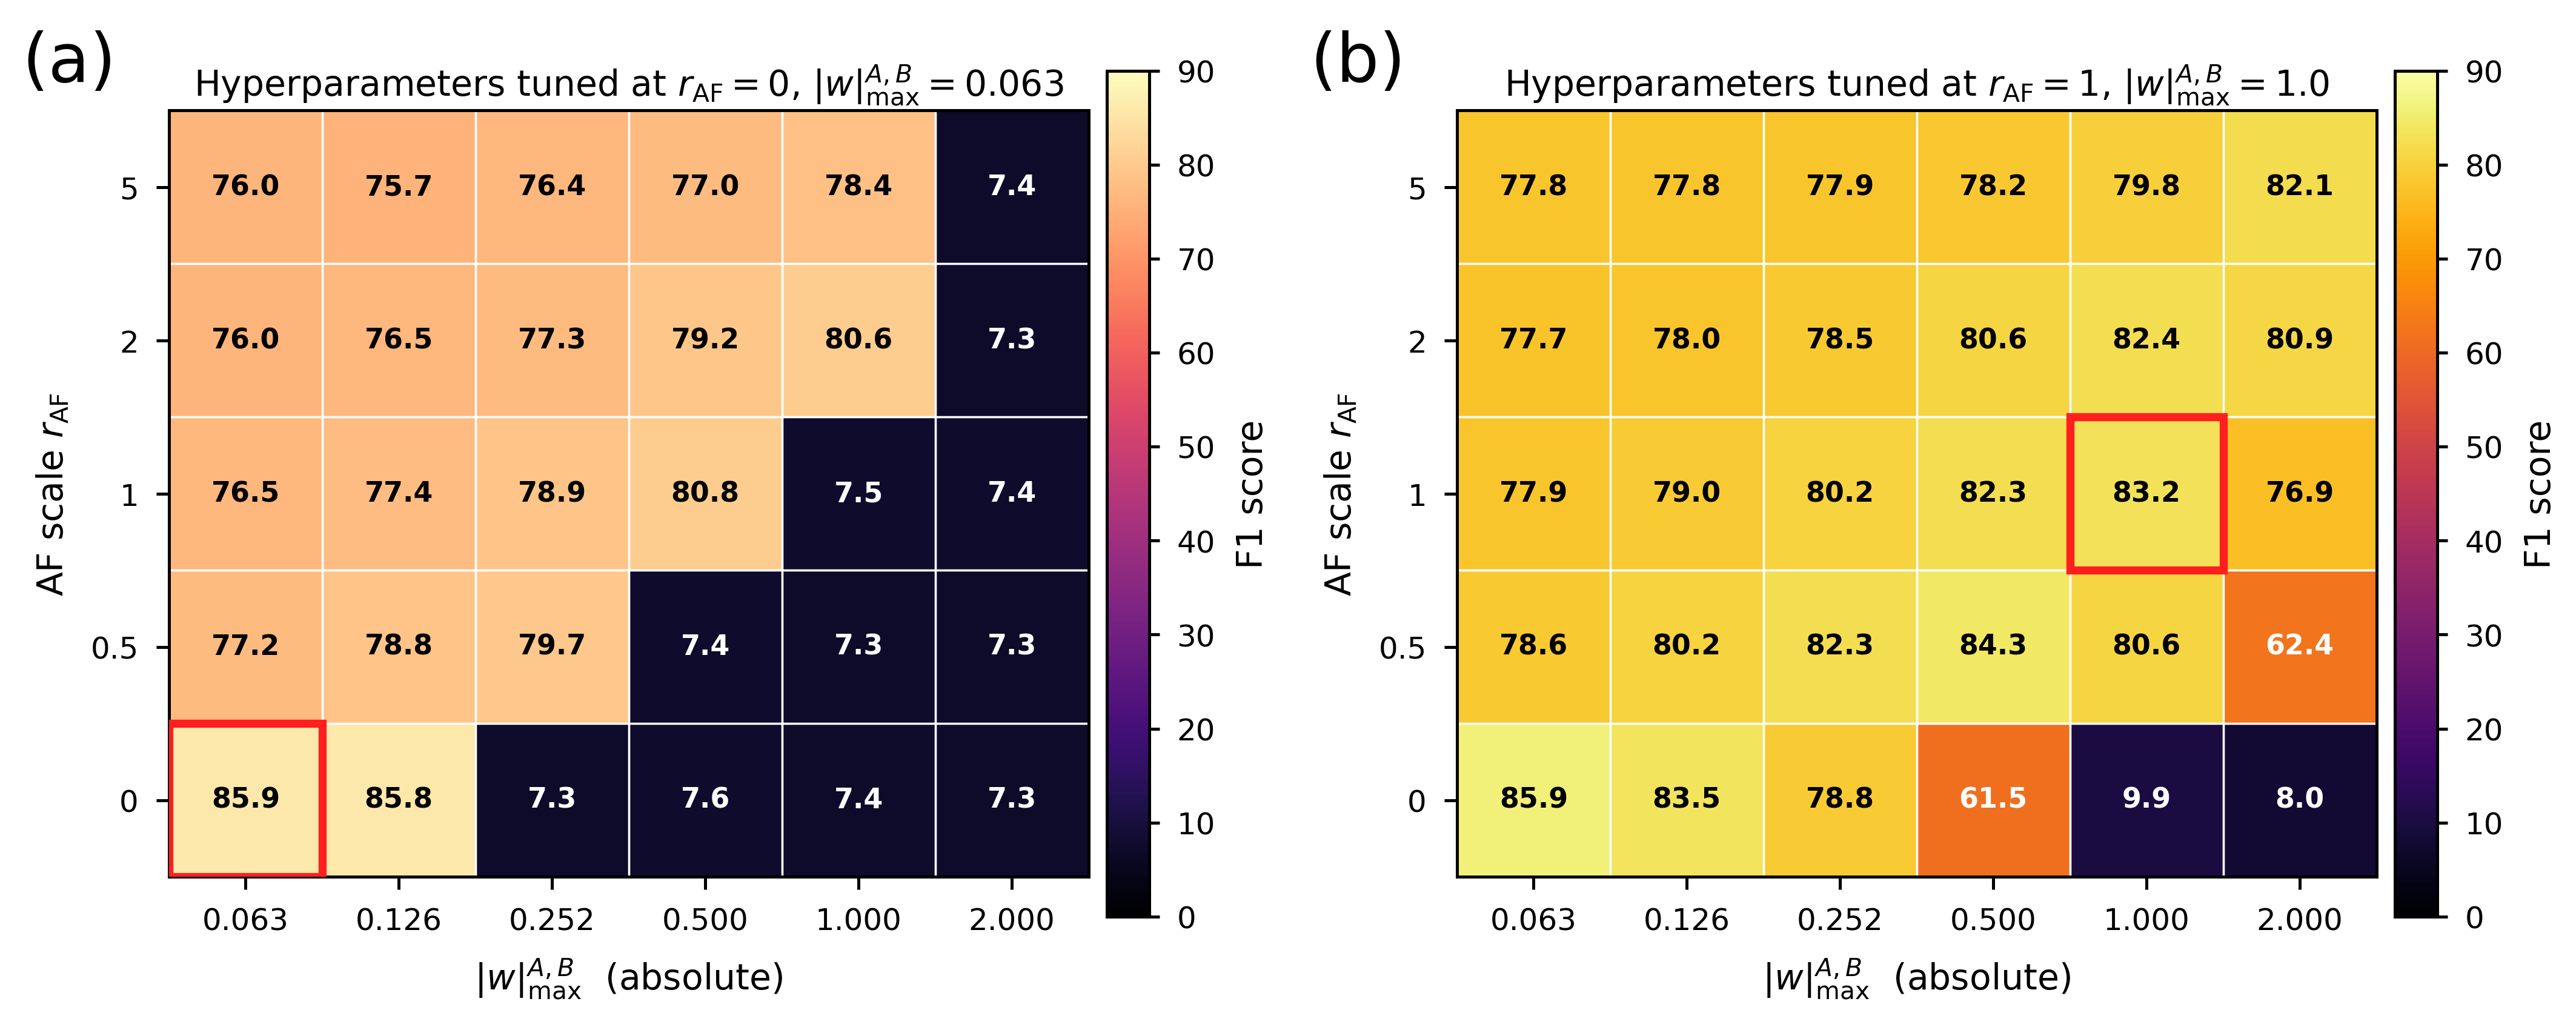
\includegraphics[width=0.98\textwidth]{sup_fig6_3.png}                                                  
    \caption{\textbf{Asymmetry-factor scale versus auxiliary weight bound.}
    F1 maps over the auxiliary weight bound \(|w|_{\max}^{A,B}\) (absolute values; shared axis across panels) and the asymmetry-factor scale \(r_{\mathrm{AF}}\) at \(r\!=\!32\) with zero noise/variation, with \(\Delta w_{\min}\) scaled to hold the 10-bit auxiliary level count fixed; dark cells denote failed training (F1\(\approx\)7, the untrained-model level) and the red box marks each panel's optimized operating point.
    (a) Hyperparameters optimized at \(r_{\mathrm{AF}}\!=\!0\) attain \(F_1\!=\!85.9\) at \((|w|_{\max}^{A,B},r_{\mathrm{AF}})=(0.063,0)\).
    (b) Hyperparameters optimized at \(r_{\mathrm{AF}}\!=\!1\) attain \(F_1\!=\!83.2\) at \((1.0,1)\), and recover the symmetric optimum (\(F_1\!=\!85.9\)) when evaluated at \((0.063,0)\).
    In both panels the per-row optimum and the divergence boundary shift toward larger \(|w|_{\max}^{A,B}\) as \(r_{\mathrm{AF}}\) grows---update asymmetry acts as an intrinsic soft bound that both stabilizes and rewards larger auxiliary weight ranges---defining a narrow diagonal \((|w|_{\max}^{A,B},r_{\mathrm{AF}})\) window for stable LR-TT training on analog hardware.}
                                                  
    \label{sub_fig6_3}                                                                                      
  \end{figure}                    

    \begin{figure}[t]                                                                                         
    \centering
    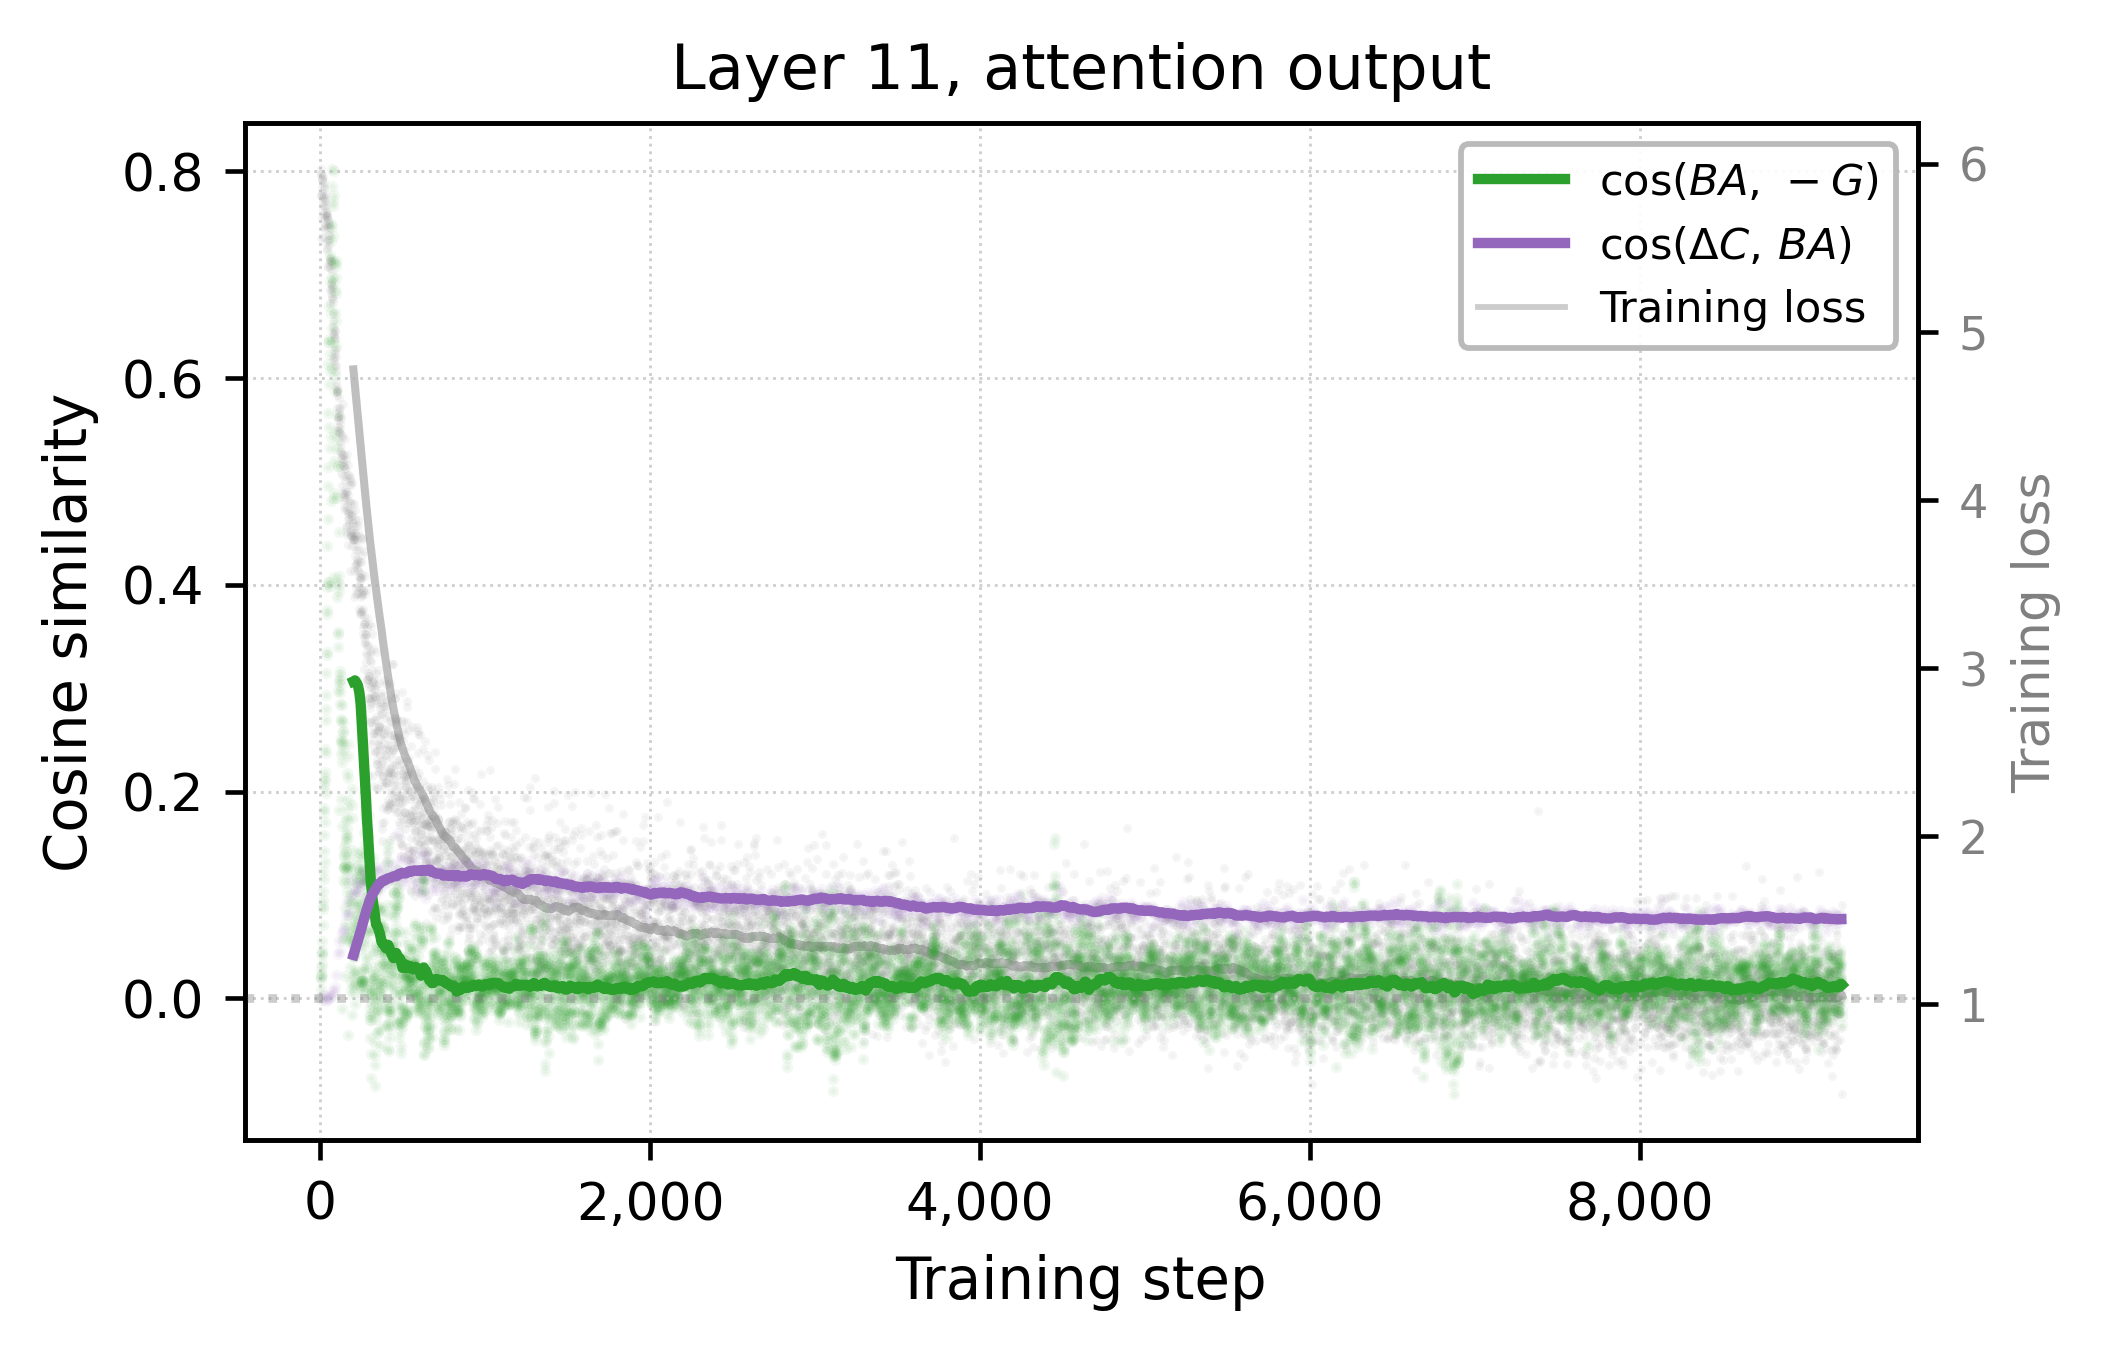
\includegraphics[width=0.98\textwidth]{sup_fig6_4.png}                                                  
    \caption{\textbf{Cosine similarity across training steps (layer 11, attention-output projection).}
    Same analysis as Fig.~5(i) for the layer-11 attention-output projection at \(r\!=\!32\): the moving average of \(\cos(BA, -G)\) between the auxiliary-tile product and the negative gradient (alignment with the descent direction), the moving average of \(\cos(\Delta C, BA)\) between the actual core-tile update and the intended transfer signal (transfer fidelity), and the training loss. Scatter points show per-step (per-transfer) raw values.}                                                
    \label{sub_fig6_4}                                                                                      
  \end{figure}          
  
    \begin{figure}[t]                                                                                         
    \centering
    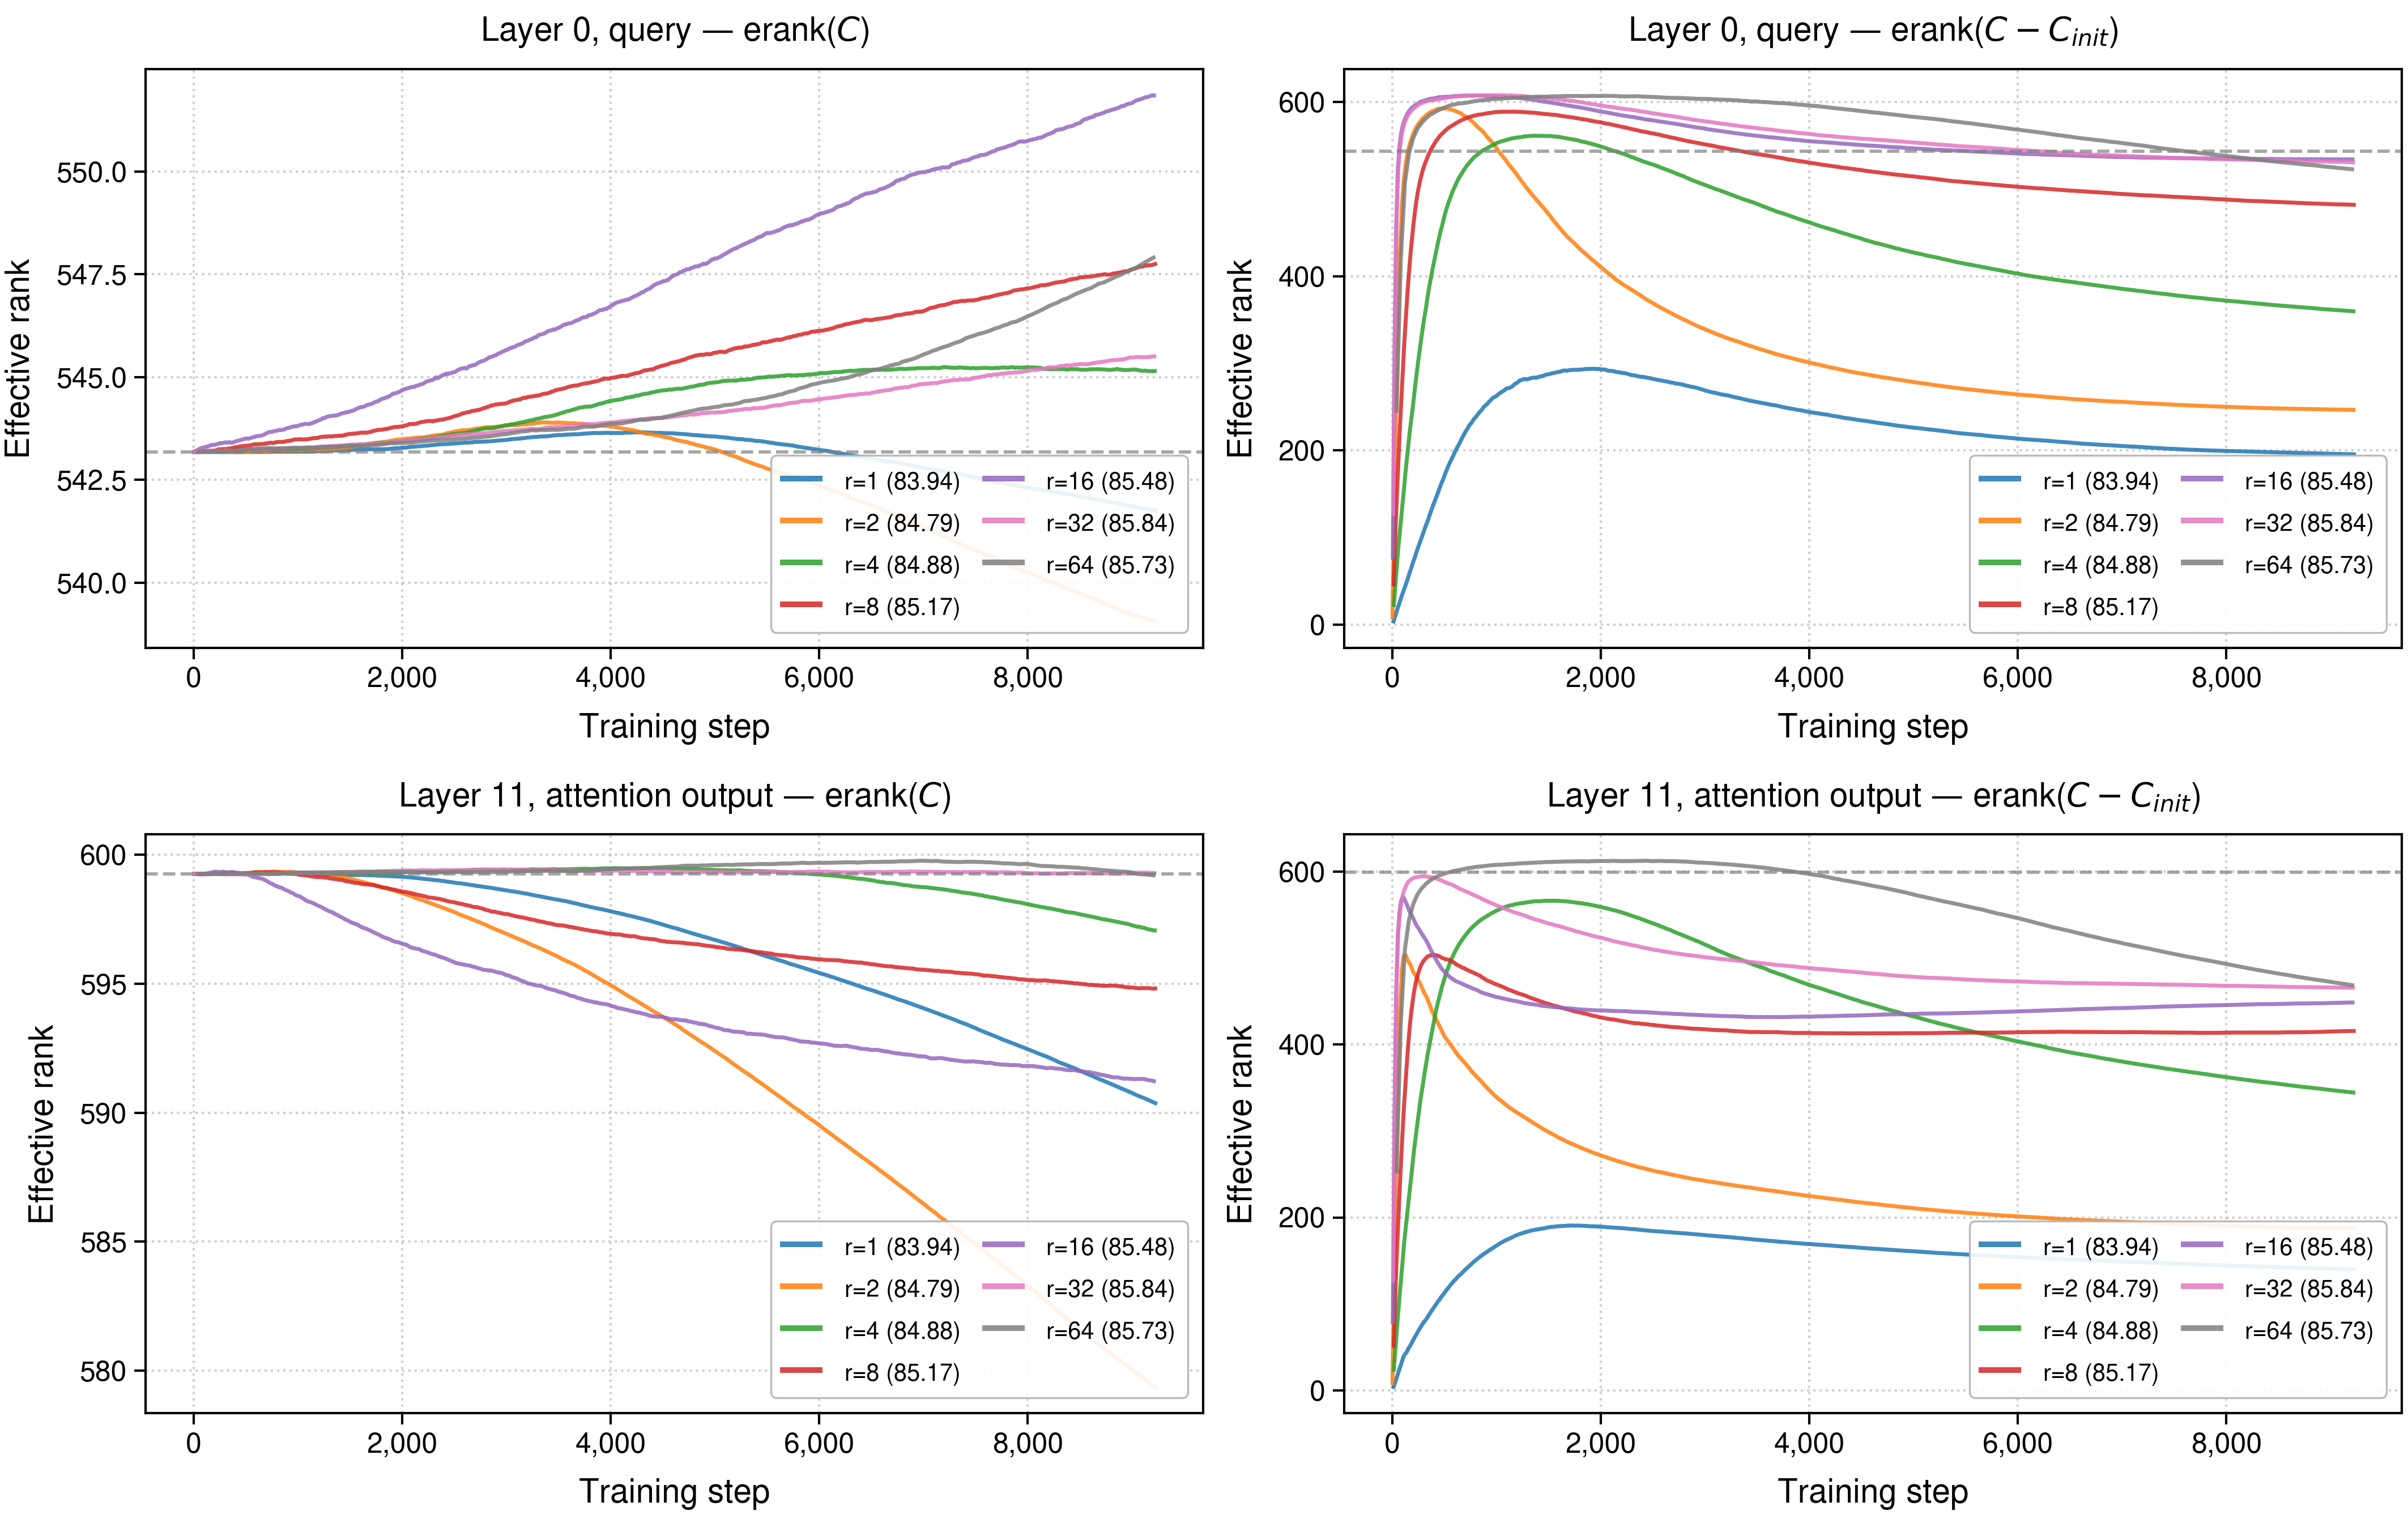
\includegraphics[width=0.98\textwidth]{sup_fig6_5.png}                                                  
    \caption{\textbf{Effective-rank trajectories of LR-TT across ranks.}
    \emph{Top row}: layer-0 query projection; \emph{bottom row}: layer-11 attention-output projection.
    In each row, the \emph{left panel} plots the effective rank of the full weight matrix $\mathrm{erank}(C)$, and the \emph{right panel} plots the effective rank of the LR-TT update $\mathrm{erank}(C-C_{\mathrm{init}})$; the gray dashed line marks $\mathrm{erank}(C_{\mathrm{init}})$ ($543.18$ for the layer-0 query, $599.26$ for the layer-11 attention output).
    All runs use analog $A$/$B$ tiles with a 10-bit constant-step-ideal pulse response ($\Delta w_{\min}=1.23\times10^{-4}$) and a 10-bit constant-step $C$-matrix ($\Delta w_{\min}=1.95\times10^{-3}$) with rank-wise stochastic transfer and per-rank optimized hyperparameters.
    For every rank, $\mathrm{erank}(C)$ in the left panels stays close to its initial value throughout training, while $\mathrm{erank}(C-C_{\mathrm{init}})$ in the right panels rises rapidly---at the highest ranks transiently exceeding $\mathrm{erank}(C_{\mathrm{init}})$---and declines during late training as successive transfers reinforce dominant singular directions.
    The dev-F1 scores corresponding to these trajectories are $83.9 / 84.8 / 84.9 / 85.2 / 85.5 / 85.8 / 85.7$ for $r=1,2,4,8,16,32,64$, saturating near $r=16$.}                                                  
    \label{sub_fig6_5}                                                                                      
  \end{figure}          



\SIEndSection

%====================================================
\section{System-level dataflow and latency--energy decomposition}
\label{sec:supp_system_decomposition}
%====================================================

\noindent
Supplementary Fig.~\ref{fig:supp_system_dataflow} summarizes the system-level dataflow used to separate the core-array, auxiliary-array, and digital contributions to latency and energy. The numerical decomposition at the nominal operating point is reported in Supplementary Table~\ref{tab:supp_component_decomposition}. Together, the figure and table specify the hardware partition, operation ordering, and component-level accounting used for the system-level analysis.

\noindent\textbf{System-level dataflow.}
Supplementary Fig.~\ref{fig:supp_system_dataflow}a shows a representative dataflow for one encoder block. The core matrix \(C\) performs the forward and backward MVMs of the mapped linear operators. The auxiliary path contains three operations: projection read, pulsed auxiliary update, and transfer from the auxiliary state to the core matrix. In LR-TT, the projection-read stage forms the low-rank update signals from the \(A\) and \(B\) factors, and the auxiliary-update stage applies pulsed updates to the factor arrays. The transfer event consolidates the accumulated auxiliary state into the core matrix and is amortized over the token positions in a training batch.

\noindent
The timing breakdown assumes serial traversal of encoder blocks and mapped matrix events, while retaining the parallelism explicitly used in the hardware partition. The \(Q/K/V\) core-array MVMs are grouped as one input-projection stage, followed by the attention-output, FFN1, and FFN2 stages. Within one LR-TT auxiliary event, the paired \(A\)- and \(B\)-factor operations are treated as one projection-read window followed by one pulsed auxiliary-update window. The same convention is used for the latency curves in Supplementary Fig.~\ref{fig:supp_system_dataflow}b and the component decomposition in Supplementary Table~\ref{tab:supp_component_decomposition}.

\noindent\textbf{Latency decomposition.}
For the all-layer mapping, the total latency per token is decomposed as
\begin{equation}
L_{\mathrm{tot}}(S)
=
L_{\mathrm{core}}
+
L_{\mathrm{aux}}
+
L_{\mathrm{attn}}(S)
+
L_{\mathrm{other}},
\label{eq:supp_total_latency}
\end{equation}
where \(L_{\mathrm{core}}\) is the core-array MVM latency, \(L_{\mathrm{aux}}\) is the auxiliary-path latency, \(L_{\mathrm{attn}}(S)\) is the sequence-length-dependent digital attention latency, and \(L_{\mathrm{other}}\) is the latency of the remaining digital operations. The core-array latency is
\begin{equation}
L_{\mathrm{core}}
=
2N_{\mathrm{blk}}\,n_{\mathrm{core}}\,T_{\mathrm{MVM}},
\label{eq:supp_core_latency}
\end{equation}
where the factor of two accounts for forward and backward MVMs. The LR-TT auxiliary latency is
\begin{equation}
L_{\mathrm{aux}}
=
N_{\mathrm{mat}}
\left(t_{\mathrm{proj}}+BL\,t_{\mathrm{pulse}}\right)
+
L_{\mathrm{xfer}},
\label{eq:supp_aux_latency}
\end{equation}
where \(N_{\mathrm{mat}}\) is the number of mapped matrices, \(t_{\mathrm{proj}}\) is the projection-read window, \(BL\,t_{\mathrm{pulse}}\) is the pulsed auxiliary-update window, and \(L_{\mathrm{xfer}}\) is the amortized transfer latency.

\noindent
The digital attention operation count is
\begin{equation}
O_{\mathrm{attn}}(S)
=
N_{\mathrm{blk}}
\left(
12DS
+
2C_{\mathrm{sm}}HS
\right),
\label{eq:supp_attn_ops}
\end{equation}
and is converted to latency by \(L_{\mathrm{attn}}(S)=O_{\mathrm{attn}}(S)/P_{\mathrm{dig}}\). The remaining digital operations are counted as
\begin{equation}
O_{\mathrm{other}}
=
N_{\mathrm{LN}}C_{\mathrm{LN}}D
+
N_{\mathrm{blk}}C_{\mathrm{GELU}}D_{\mathrm{ff}}
+
N_{\mathrm{blk}}N_{\mathrm{res}}C_{\mathrm{res}}D,
\label{eq:supp_other_ops}
\end{equation}
with \(L_{\mathrm{other}}=O_{\mathrm{other}}/P_{\mathrm{dig}}\). These terms correspond to LayerNorm, GeLU, and residual additions.

\noindent\textbf{Energy decomposition.}
The energy per token is decomposed analogously as
\begin{equation}
E_{\mathrm{tot}}(S)
=
E_{\mathrm{core}}
+
E_{\mathrm{aux}}
+
E_{\mathrm{attn}}(S)
+
E_{\mathrm{other}}.
\label{eq:supp_total_energy}
\end{equation}
The core and auxiliary analog components are obtained from their primitive-operation counts and the analog energy unit, with the auxiliary-update term scaled by the update-to-MVM energy ratio. The digital components are obtained from
\begin{equation}
E_{\mathrm{attn}}(S)=O_{\mathrm{attn}}(S)\varepsilon_{\mathrm{dig}},
\qquad
E_{\mathrm{other}}=O_{\mathrm{other}}\varepsilon_{\mathrm{dig}}.
\label{eq:supp_digital_energy}
\end{equation}
This decomposition keeps the core-array, auxiliary-array, and digital contributions explicit in both the latency and energy estimates.

\begin{table}[!htbp]
\centering
\caption{\textbf{Component-level latency and energy decomposition at the nominal operating point.}
All values are reported per token for the all-layer mapping at \(S=384\), \(r=32\), and \(BL=31\). The table lists the counting expression, operation count, latency, energy, and modelling basis for each component.}
\label{tab:supp_component_decomposition}
{\small
\renewcommand{\arraystretch}{1.18}
\setlength{\tabcolsep}{3.6pt}
\begin{tabularx}{\textwidth}{@{}p{2.9cm}Y r r r p{3.2cm}@{}}
\toprule
\textbf{Component} &
\textbf{Counting expression} &
\textbf{Ops/token} &
\textbf{Latency/token} &
\textbf{Energy/token} &
\textbf{Modelling basis} \\
&
&
\textbf{[\(\times10^{6}\)]} &
\textbf{[\(\mu\mathrm{s}\)]} &
\textbf{[\(\mu\mathrm{J}\)]} &
\\
\midrule
Core-array MVM &
\(O_{\mathrm{core}}=\sum_{\ell\in\mathcal{L}}4M_{\ell}N_{\ell}\), 
\(L_{\mathrm{core}}=2N_{\mathrm{blk}}n_{\mathrm{core}}T_{\mathrm{MVM}}\) &
339.74 & 9.60 & 26.54 &
Calibrated AIMC tile and HERMES-class core \cite{klein2023alpine,khaddam2022hermescore} \\
Auxiliary projection read &
\(O_{\mathrm{proj}}=\sum_{\ell\in\mathcal{L}}2r(M_{\ell}+N_{\ell})\), 
\(L_{\mathrm{proj}}=N_{\mathrm{mat}}T_{\mathrm{MVM}}\) &
10.62 & 7.20 & 0.83 &
Low-rank projection read and analog MVM primitive \cite{hu2021lora,klein2023alpine} \\
Auxiliary pulse update &
\(O_{\mathrm{upd}}=\sum_{\ell\in\mathcal{L}}2r(M_{\ell}+N_{\ell})\), 
\(L_{\mathrm{upd}}=N_{\mathrm{mat}}BL\,t_{\mathrm{pulse}}\) &
10.62 & 11.16 & 0.83 &
Pulsed-update primitive \cite{gokmen2016rpu,rasch2024fastrobust} \\
Auxiliary-to-core transfer &
Amortized transfer from the auxiliary state to the core matrix over \(B\times S\) token positions &
\(<0.001\) & \(<0.001\) & \(<0.001\) &
Tiki-Taka transfer schedule \cite{gokmen2020tikitaka,rasch2024fastrobust} \\
Digital attention &
\(O_{\mathrm{attn}}(S)=N_{\mathrm{blk}}(12DS+2C_{\mathrm{sm}}HS)\) &
42.91 & 33.52 & 42.91 &
Transformer attention count and digital reference \cite{vaswani2017attention,horowitz2014computing} \\
Digital other operations &
\(O_{\mathrm{other}}=N_{\mathrm{LN}}C_{\mathrm{LN}}D+N_{\mathrm{blk}}C_{\mathrm{GELU}}D_{\mathrm{ff}}+N_{\mathrm{blk}}N_{\mathrm{res}}C_{\mathrm{res}}D\) &
1.03 & 0.80 & 1.03 &
LayerNorm, GeLU, residual additions, and digital reference \cite{horowitz2014computing} \\
\midrule
\textbf{Total} &
--- &
\textbf{404.91} & \textbf{62.29} & \textbf{72.14} &
--- \\
\bottomrule
\end{tabularx}
}
\vspace{0.35em}

\begin{minipage}{0.97\textwidth}
\footnotesize
\emph{Notes.}
\(\mathcal{L}\) denotes the mapped matrices in the all-layer setting, including repetition across encoder blocks.
\(N_{\mathrm{blk}}=12\), \(N_{\mathrm{mat}}=72\), and \(n_{\mathrm{core}}=4\).
The digital terms use \(P_{\mathrm{dig}}\) for latency conversion and \(\varepsilon_{\mathrm{dig}}\) for energy conversion.
The auxiliary-update energy uses the nominal update-to-MVM energy ratio.
The transfer contribution is below \(10^{-3}\) in the displayed units after amortization.
\end{minipage}
\end{table}
\FloatBarrier

\noindent\textbf{Component-level decomposition.}
Supplementary Table~\ref{tab:supp_component_decomposition} gives the numerical decomposition for the nominal operating point shown in Supplementary Fig.~\ref{fig:supp_system_dataflow}b,c. The table separates the total latency and energy into core-array MVM, auxiliary projection read, auxiliary pulse update, auxiliary-to-core transfer, digital attention, and remaining digital operations. Each row lists the counting expression, per-token operation count, latency, energy, and modelling basis. The analog components are tied to the calibrated AIMC tile and HERMES-class core assumptions \cite{klein2023alpine,khaddam2022hermescore}, the auxiliary update uses pulsed-update primitives \cite{gokmen2016rpu,rasch2024fastrobust}, and the digital components use transformer operation counts and first-order digital reference parameters \cite{vaswani2017attention,horowitz2014computing}. This table provides a component-by-component check of the decompositions in Supplementary Eqs.~\eqref{eq:supp_total_latency} and \eqref{eq:supp_total_energy}.

\begin{figure}[t]
  \centering
  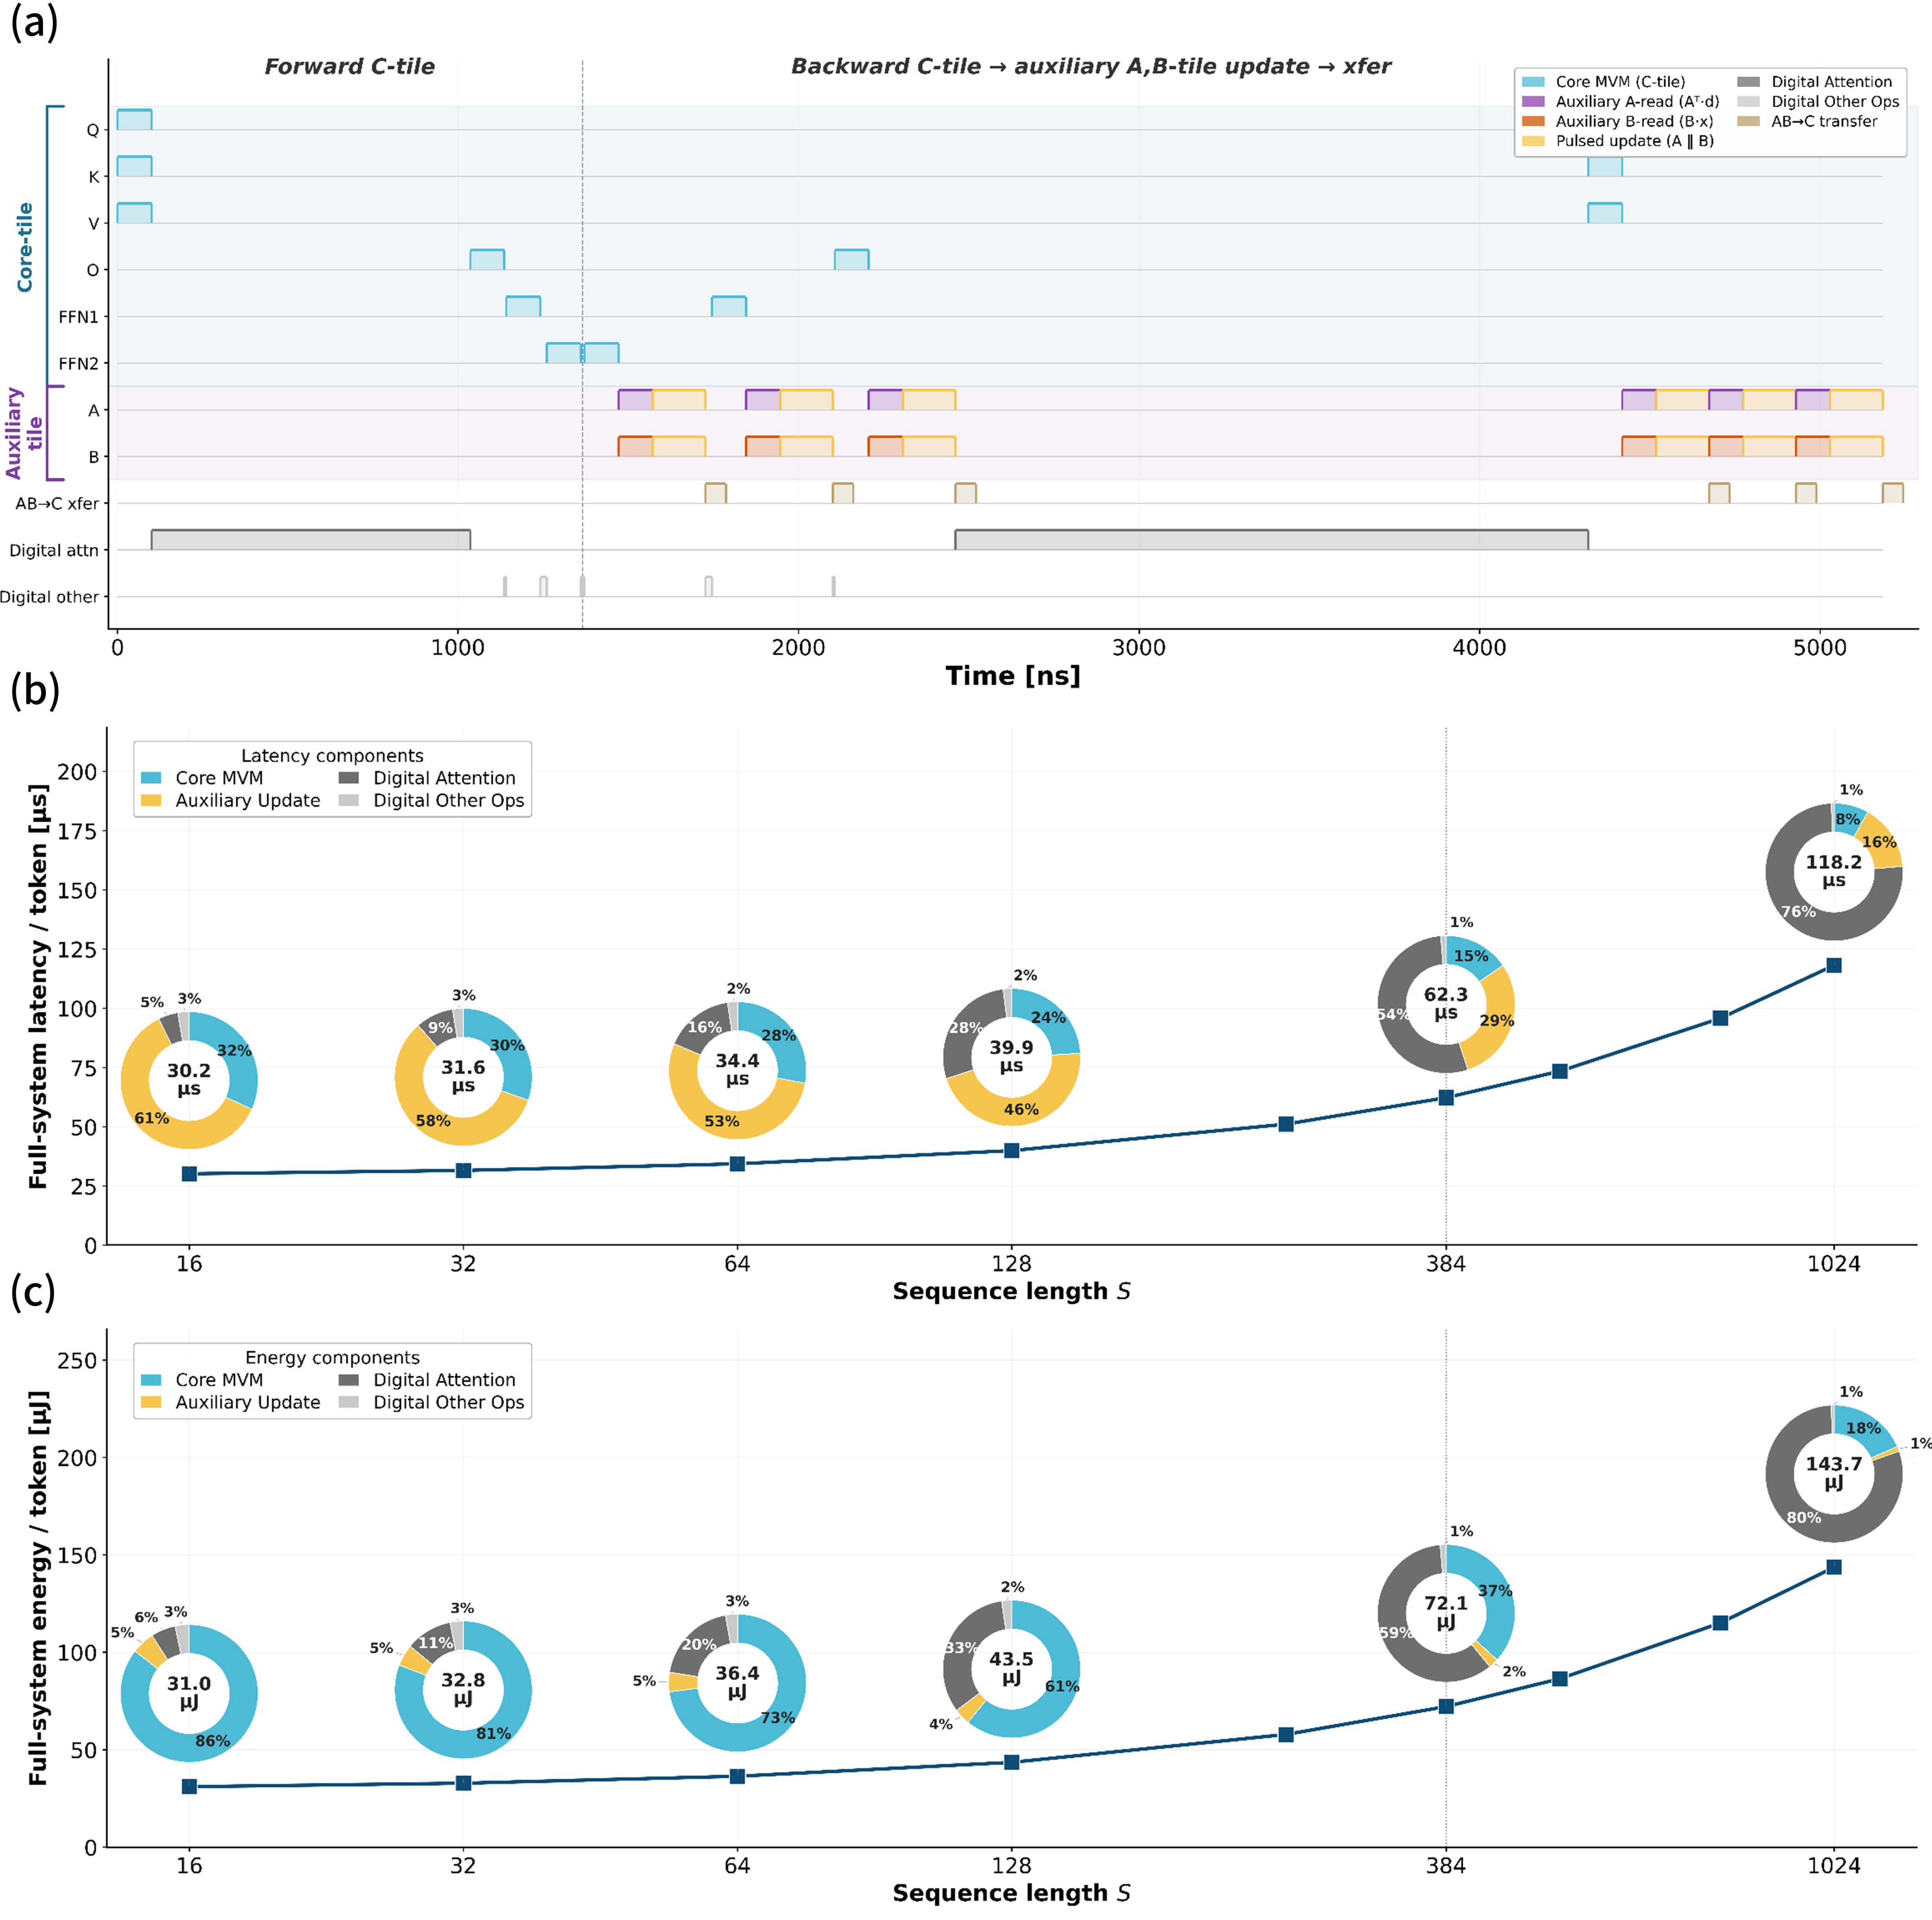
\includegraphics[width=0.98\textwidth]{sup_fig7.png}
  \caption{\textbf{System-level dataflow and latency--energy decomposition.}
  (a) Representative dataflow and timing breakdown for one encoder block under the core--auxiliary--digital partition.
  Core-array MVMs, auxiliary projection reads, pulsed auxiliary updates, transfer events, digital attention, and remaining digital operations are shown as separate components.
  (b) Latency per token versus sequence length for the all-layer mapping at $r=32$ and $BL=31$, with component fractions shown at each sequence length.
  (c) Energy per token versus sequence length under the same operating point and component grouping.}
  \label{fig:supp_system_dataflow}
\end{figure}


\SIEndSection

%====================================================
\clearpage
\section{Simulation setup and implementation details}
\label{sec:S8}
%====================================================

\noindent
This section summarizes the simulator configuration and training settings used for the MNIST scratch-training and BERT-base SQuAD fine-tuning experiments. All simulations involving array-based operations were performed with the IBM Analog Hardware Acceleration Kit (AIHWKIT) using custom LR-TT RPU configurations \cite{rasch2021aihwkit,legallo2023aihwkit}. We first define the simulator quantities used for weight precision, device variation, update asymmetry, pulse noise, I/O parameterization, and pulsed updates. The corresponding numerical settings are listed in Supplementary Table~\ref{tab:S8_hardware_simulator}, and the task-specific model and training settings are listed in Supplementary Tables~\ref{tab:S8_mnist_training} and~\ref{tab:S8_bert_training}.

\noindent\textbf{Weight precision.}
For an array \(q\) with programmable weight range \([w_{\min}^{q},w_{\max}^{q}]\), the nominal update granularity associated with a \(b_w\)-bit weight is defined as
\begin{equation}
\Delta w_{\min}^{q}(b_w)
=
\frac{w_{\max}^{q}-w_{\min}^{q}}{2^{b_w}} .
\label{eq:S8_weight_bit}
\end{equation}
Thus, the weight-bit setting controls the programming granularity at fixed dynamic range. In the core-array precision study, \(q=C\); in auxiliary-array range or precision studies, \(q\) denotes the corresponding auxiliary array.

\noindent\textbf{Device variation and update asymmetry.}
For each cross-point \((i,j)\), static device-to-device variation is applied to the device bounds and minimum update steps. The upper and lower bounds are modeled as
\begin{equation}
b^{\max}_{ij}=w_{\max}\left(1+\sigma_{b^{\max}}\xi_{ij}^{\max}\right),
\qquad
b^{\min}_{ij}=w_{\min}\left(1+\sigma_{b^{\min}}\xi_{ij}^{\min}\right),
\label{eq:S8_bound_dtod}
\end{equation}
where \(\xi\sim\mathcal{N}(0,1)\). Here, \(\sigma_{b^{\max}}\) and \(\sigma_{b^{\min}}\) denote device-to-device variation of the upper and lower bounds, respectively. The directional minimum update steps are
\begin{equation}
\Delta w^{+}_{ij}
=
\Delta w_{\min}
\left(g_{ij}+r_{ij}+\beta^{+}\right),
\qquad
\Delta w^{-}_{ij}
=
\Delta w_{\min}
\left(g_{ij}-r_{ij}+\beta^{-}\right),
\label{eq:S8_directional_step}
\end{equation}
where \(g_{ij}=1+\sigma_{\Delta}^{\mathrm{d2d}}\xi_{ij}^{\Delta}\) denotes device-to-device update-step gain variation, \(r_{ij}=\sigma_{\mathrm{ud}}^{\mathrm{d2d}}\xi_{ij}^{\mathrm{ud}}\) denotes device-specific directional imbalance, and \(\beta^{+},\beta^{-}\) denote systematic directional bias terms.

\noindent
The update asymmetry factor used in the main text is implemented through the directional linear-step slopes. For an asymmetry-factor scale \(r_{\mathrm{AF}}\), the nominal directional slopes are scaled as
\begin{equation}
\widetilde{\gamma}^{+}_{ij}
=
r_{\mathrm{AF}}
\left(
\bar{\gamma}^{+}
+
\sigma_{\gamma^{+}}\xi_{ij}^{\gamma^{+}}
\right),
\qquad
\widetilde{\gamma}^{-}_{ij}
=
r_{\mathrm{AF}}
\left(
\bar{\gamma}^{-}
+
\sigma_{\gamma^{-}}\xi_{ij}^{\gamma^{-}}
\right),
\label{eq:S8_af_ratio}
\end{equation}
where \(\bar{\gamma}^{+}\) and \(\bar{\gamma}^{-}\) are nominal directional slopes and \(\sigma_{\gamma^{+}},\sigma_{\gamma^{-}}\) denote their device-to-device variations. For the core-array nonlinearity study, \(\mathrm{AF}^{C}\) denotes the common directional-slope magnitude applied to the core array. The effective slopes used in the linear-step update are normalized by the device range:
\begin{equation}
\Gamma^{+}_{ij}
=
-\frac{|\widetilde{\gamma}^{+}_{ij}|\,\Delta w^{+}_{ij}}{w_{\max}},
\qquad
\Gamma^{-}_{ij}
=
-\frac{|\widetilde{\gamma}^{-}_{ij}|\,\Delta w^{-}_{ij}}{w_{\min}} .
\label{eq:S8_effective_slope}
\end{equation}
In the BERT sensitivity study, the asymmetry-factor scale corresponds to \(r_{\mathrm{AF}}\) in Supplementary Eq.~\eqref{eq:S8_af_ratio}. The noise/variation scale scales the auxiliary-device noise and variation amplitudes relative to the nominal 6T1C setting:
\begin{equation}
\boldsymbol{\sigma}_{\mathrm{aux}}(r_{\mathrm{noise}})
=
r_{\mathrm{noise}}\,
\boldsymbol{\sigma}_{\mathrm{aux}}^{(0)},
\qquad
\boldsymbol{\sigma}_{\mathrm{aux}}^{(0)}
=
\left\{
\sigma_{\Delta}^{\mathrm{d2d}},
\sigma_{\mathrm{ud}}^{\mathrm{d2d}},
\sigma_{b^{\max}},
\sigma_{b^{\min}},
\sigma_{\gamma^{+}},
\sigma_{\gamma^{-}},
\bar{\sigma}_{\mathrm{pulse}}
\right\}.
\label{eq:S8_noise_ratio}
\end{equation}
Thus, \(r_{\mathrm{noise}}=1\) corresponds to the nominal auxiliary-device noise and variation setting listed in Supplementary Table~\ref{tab:S8_hardware_simulator}.

\noindent\textbf{Per-pulse update.}
For one programming pulse, the auxiliary-array state is updated by a direction-dependent linear-step rule,
\begin{equation}
w_{ij}\leftarrow
\begin{cases}
w_{ij}
+
\Gamma^{+}_{ij}w_{ij}
+
\Delta w^{+}_{ij}\left(1+\sigma_{\mathrm{pulse}}\xi\right),
& \text{positive update},\\[4pt]
w_{ij}
-
\Gamma^{-}_{ij}w_{ij}
-
\Delta w^{-}_{ij}\left(1+\sigma_{\mathrm{pulse}}\xi\right),
& \text{negative update},
\end{cases}
\label{eq:S8_per_pulse_update}
\end{equation}
followed by clipping to the bounds in Supplementary Eq.~\eqref{eq:S8_bound_dtod}. The pulse-to-pulse standard deviation \(\sigma_{\mathrm{pulse}}\) represents cycle-to-cycle stochasticity during programming, whereas the device-to-device terms in Supplementary Eqs.~\eqref{eq:S8_bound_dtod}--\eqref{eq:S8_af_ratio} are sampled once per cross-point and remain fixed during training. If apparent write noise is enabled, the read weight is modeled as
\begin{equation}
w^{\mathrm{app}}_{ij}
=
w_{ij}
+
\sigma_{\mathrm{wn}}\Delta w_{\min}\xi ,
\label{eq:S8_write_noise}
\end{equation}
where \(\sigma_{\mathrm{wn}}\) is the apparent write-noise standard deviation; this term is disabled in the reported settings.

\noindent\textbf{I/O parameterization.}
The input precision \(b_{\mathrm{DAC}}\) corresponds to the DAC precision and the output precision \(b_{\mathrm{ADC}}\) corresponds to the ADC precision. Their normalized quantization steps are
\begin{equation}
\Delta_{\mathrm{DAC}}=\frac{1}{2^{b_{\mathrm{DAC}}}-2},
\qquad
\Delta_{\mathrm{ADC}}=\frac{1}{2^{b_{\mathrm{ADC}}}-2}.
\label{eq:S8_io_resolution}
\end{equation}
With absolute-maximum input scaling \(s_x=\max_i|x_i|\), the input to the array is quantized as
\begin{equation}
\hat{x}_i
=
\Delta_{\mathrm{DAC}}
\operatorname{round}
\left[
\frac{\operatorname{clip}(x_i/s_x,-B_{\mathrm{DAC}},B_{\mathrm{DAC}})}
{\Delta_{\mathrm{DAC}}}
\right].
\label{eq:S8_input_quant}
\end{equation}
The output is computed as
\begin{equation}
\tilde{y}_j
=
\sum_i w_{ji}\hat{x}_i
+
\sigma_{\mathrm{out}}\xi_j,
\qquad
\hat{y}_j
=
s_x\Delta_{\mathrm{ADC}}
\operatorname{round}
\left[
\frac{\operatorname{clip}(\tilde{y}_j,-B_{\mathrm{ADC}},B_{\mathrm{ADC}})}
{\Delta_{\mathrm{ADC}}}
\right],
\label{eq:S8_output_quant}
\end{equation}
where \(\sigma_{\mathrm{out}}\) is the output-referred I/O noise. Forward operations use absolute-maximum input scaling and iterative output-bound rescaling, whereas backward operations use the same quantization model without iterative bound rescaling.

\noindent\textbf{Pulsed update encoding.}
For an outer-product update with input component \(x_j\), error component \(d_i\), learning rate \(\eta\), and update granularity \(\Delta w_{\min}\), the pulse length is bounded by
\begin{equation}
\mathrm{BL}_{ij}
=
\min
\left(
\left\lceil
\frac{\eta |x_j||d_i|}{\Delta w_{\min}}
\right\rceil,
\mathrm{BL}_{\max}
\right).
\label{eq:S8_bl}
\end{equation}
Stochastic pulse trains are generated with probabilities proportional to the scaled input and error magnitudes, and an update pulse is applied when the two streams coincide. This preserves the expected outer-product update while using bounded pulse length.

\noindent\textbf{Common simulator configuration.}
Supplementary Table~\ref{tab:S8_hardware_simulator} summarizes the common AIHWKIT configuration used for LR-TT simulations. The listed 6T1C-calibrated auxiliary-array parameters define the baseline device used across the MNIST and BERT-base studies. BERT-base training and diagnostics both use the 8-bit DAC/ADC I/O model with Gaussian output noise \(\sigma_{\mathrm{out}}=0.04\) on forward and backward MVMs; the diagnostic studies additionally vary the DAC/ADC precision from 4 to 8 bits. For the BERT-base auxiliary-device study, the auxiliary weight range is varied over \(|w|_{\max}^{A,B}\in[0.01,1.0]\), with \(\Delta w_{\min}\) adjusted according to the target weight precision using Supplementary Eq.~\eqref{eq:S8_weight_bit}. For the MNIST core-array study, the core precision study uses \(b_w\in\{5,6,7,8,9,10\}\), and the core nonlinearity study uses \(\mathrm{AF}^{C}\in\{0,0.5,1,2,5,10\}\). The BERT-base AF-ratio and noise-ratio studies scale the auxiliary-array baseline slopes and noise/variation amplitudes defined in Supplementary Table~\ref{tab:S8_hardware_simulator} according to Supplementary Eqs.~\eqref{eq:S8_af_ratio} and~\eqref{eq:S8_noise_ratio}.

%----------------------------------------------------
\begin{table}[!htbp]
\centering
\caption{\textbf{Common simulator, device, I/O, and update settings for LR-TT.}
The table lists the shared AIHWKIT simulator configuration and the baseline numerical parameters used unless a study-specific condition modifies the corresponding quantity.}
\label{tab:S8_hardware_simulator}
\small
\renewcommand{\arraystretch}{1.10}
\setlength{\tabcolsep}{4.0pt}
\begin{tabularx}{\linewidth}{p{3.0cm}Y}
\toprule
\rowcolor{HeadGray}
\textbf{Component} & \textbf{Setting} \\
\midrule
Simulation framework &
AIHWKIT v0.9.0 with a custom LR-TT RPU configuration. Mapped linear layers use array MVM and pulsed auxiliary-array update; non-matrix operations are evaluated digitally. \\
\midrule
Auxiliary-array device &
Baseline 6T1C-calibrated linear-step device: \(|w|_{\max}^{A,B}=1\), \(\Delta w_{\min}=0.001981\), \(\bar{\gamma}^{+}=0.1678\), \(\bar{\gamma}^{-}=0.1410\), and \(\bar{\sigma}_{\mathrm{pulse}}=0.3\). BERT auxiliary-range studies use \(|w|_{\max}^{A,B}\in[0.01,1.0]\) with \(\Delta w_{\min}\) set by Supplementary Eq.~\eqref{eq:S8_weight_bit}. \\
\midrule
Auxiliary-array variation &
\(\sigma_{\Delta}^{\mathrm{d2d}}=0.1\), \(\sigma_{\mathrm{ud}}^{\mathrm{d2d}}=0.01\), \(\sigma_{b^{\max}}=\sigma_{b^{\min}}=0.05\), \(\sigma_{\gamma^{+}}=\sigma_{\gamma^{-}}=0.05\), and \(\sigma_{\mathrm{wn}}=0\). BERT noise-ratio studies multiply these baseline amplitudes by \(r_{\mathrm{noise}}\). \\
\midrule
Core-array device &
Baseline core array: \(|w|_{\max}^{C}=1\) (raw-tile bound; the effective model weight is recovered through a per-tile scaling factor calibrated to the pretrained weight range), \(\Delta w_{\min}=0.001\), \(\bar{\gamma}^{+}=\bar{\gamma}^{-}=0\), \(\sigma_{\Delta}^{\mathrm{d2d}}=0\), \(\sigma_{\mathrm{pulse}}=0\), and \(\sigma_{\mathrm{wn}}=0\). MNIST core studies use \(b_w\in\{5,6,7,8,9,10\}\), \(\Delta w_{\min}^{C}=2/2^{b_w}\), and \(\mathrm{AF}^{C}\in\{0,0.5,1,2,5,10\}\). \\
\midrule
I/O parameter &
MNIST training I/O: \(b_{\mathrm{DAC}}=7\), \(b_{\mathrm{ADC}}=9\), \(B_{\mathrm{DAC}}=1.0\), \(B_{\mathrm{ADC}}=12.0\), \(\sigma_{\mathrm{out}}=0\). All BERT training and diagnostics use \(b_{\mathrm{DAC}}=b_{\mathrm{ADC}}=8\), \(B_{\mathrm{DAC}}=1.0\), \(B_{\mathrm{ADC}}=12.0\), and Gaussian output noise \(\sigma_{\mathrm{out}}=0.04\) on both forward and backward MVMs, applied identically to every mapped array (adapted and frozen); the one-epoch I/O-precision probe of Fig.~5(d) additionally varies \(b_{\mathrm{DAC}},b_{\mathrm{ADC}}\in\{4,5,6,7\}\) per operator group. Forward MVM uses absolute-maximum scaling with iterative bound rescaling; backward MVM uses the same precision without iterative bound rescaling. Mapped \(768\times768\) layers are partitioned into \(2\times2\) sub-arrays of \(384\times384\) (maximum array size 512). \\
\midrule
Pulsed-update parameter &
\(\mathrm{BL}_{\max}=31\), fixed-length stochastic-compressed pulse encoding, and dynamic rescaling of input/error amplitudes. \\
\bottomrule
\end{tabularx}
\end{table}
\FloatBarrier

\noindent\textbf{MNIST model and training setting.}
Supplementary Table~\ref{tab:S8_mnist_training} lists the task, network architecture, mapped-layer partition, LR-TT configuration, and training setting used for the MNIST scratch-training experiments. The table is limited to model and training hyperparameters; reset/retention analysis is provided in Supplementary Section~\ref{sec:S5}.

%----------------------------------------------------
\begin{table}[!htbp]
\centering
\caption{\textbf{MNIST network mapping and training settings.}
The table lists the task, model, mapped-layer configuration, LR-TT setting, and training setting used for the small-scale scratch-training experiments.}
\label{tab:S8_mnist_training}
\small
\renewcommand{\arraystretch}{1.10}
\setlength{\tabcolsep}{4.0pt}
\begin{tabularx}{\linewidth}{p{3.0cm}Y}
\toprule
\rowcolor{HeadGray}
\textbf{Component} & \textbf{Setting} \\
\midrule
Task and dataset &
MNIST handwritten-digit classification with 60,000 training images and 10,000 test images. Inputs are flattened from \(28\times28\) pixels and normalized with mean 0.1307 and standard deviation 0.3081. \\
\midrule
Model architecture &
Two-layer MLP with a \(784\rightarrow256\) hidden layer, ReLU nonlinearity, a \(256\rightarrow10\) classifier layer, and LogSoftmax output. \\
\midrule
Mapped linear layers &
The \(784\rightarrow256\) layer is mapped to an LR-TT block with auxiliary \(A/B\) arrays and a \(C\) core array. The classifier layer is evaluated in a floating-point path. \\
\midrule
Digital path &
ReLU, LogSoftmax, loss evaluation, and classifier operations outside the LR-TT block are evaluated digitally. \\
\midrule
LR-TT configuration &
Core-array-only forward path with \(\gamma=0\). Rank \(r\in\{1,4,8,16,32,64\}\), transfer interval \(\tau\in\{1,10,50,100,500,1000\}\), and fixed transfer learning rate \(\eta_{\mathrm{tr}}=0.010/r\) for the fixed-hyperparameter runs. \\
\midrule
Training setting &
Analog SGD with negative log-likelihood loss, batch size 64, 30 epochs, learning rate 0.3 for the fixed-hyperparameter runs, and step learning-rate decay with step size 10 and decay factor 0.5. \\
\bottomrule
\end{tabularx}
\end{table}
\FloatBarrier

\noindent\textbf{BERT-base SQuAD model and training setting.}
Supplementary Table~\ref{tab:S8_bert_training} lists the BERT-base SQuAD task setup using the same component structure as Supplementary Table~\ref{tab:S8_mnist_training}. This presentation separates model/training hyperparameters from the shared simulator/device settings in Supplementary Table~\ref{tab:S8_hardware_simulator} and keeps the MNIST and transformer configurations directly comparable.

\clearpage
\noindent\textbf{Practical heuristic for selecting LR-TT hyperparameters.}
The sensitivity analyses of Fig.~6c and Supplementary Figs.~\ref{sub_fig6_2} and~\ref{sub_fig6_3} suggest a practical ordering for configuring LR-TT on a new auxiliary device, taking its measured update asymmetry and noise/variation level as inputs.
(1) \emph{Fix the auxiliary weight range first.} The auxiliary bound \(|w|_{\max}^{A,B}\) is the dominant axis. Select the largest bound that stays safely inside the divergence boundary mapped in Supplementary Fig.~S9: for near-symmetric devices the optimum lies far below the core-tile range (\(|w|_{\max}^{A,B}\approx0.03\)--\(0.13\) in our setup), whereas update asymmetry acts as an intrinsic soft bound that shifts the boundary outward (\(|w|_{\max}^{A,B}\approx0.5\)--\(1.0\) at the nominal 6T1C asymmetry), with F1 recovering as the bound grows up to the boundary. In our experiments this bound absorbed essentially all of the asymmetry dependence: the remaining hyperparameters optimized at the nominal asymmetry stayed near-optimal across the full asymmetry range once the bound was re-selected per operating point, whereas the converse did not hold---settings optimized without asymmetry degraded under it (Supplementary Fig.~\ref{sub_fig6_3}). When a single configuration must cover an uncertain or spread asymmetry level, this favors fixing the remaining hyperparameters at the highest expected asymmetry and adapting only the bound.
(2) \emph{Search over the bound, not the pulse granularity.} At a fixed auxiliary bit count \(n\), the pulse granularity follows from the bound as \(\Delta w_{\min} = 2\,|w|_{\max}^{A,B}/2^{n}\). Because the optimal bound is only weakly bit-dependent, the optimal \(\Delta w_{\min}\) scales as \(2^{-n}\); a search window specified in \(\Delta w_{\min}\) and inherited from a different bit width can therefore silently exclude the optimum (re-parameterizing our 6-bit auxiliary search in these terms recovered \(+5.8\) F1).
(3) \emph{Couple the transfer interval to the dominant non-ideality.} Under update asymmetry alone, frequent transfers are favored (\(\tau=1\)--\(2\); \(\tau=24\) costs about 5 F1 at 6-bit precision), consistent with frequent consolidation limiting how far asymmetric drift can distort the accumulated update. Under significant noise/variation the preference reverses---longer accumulation intervals average stochastic updates before they reach the core tile (\(\tau=24\) is optimal at the nominal 6T1C noise level, whereas \(\tau=1\) fails, F1\(<\)40)---so the interval must be chosen at the joint operating point. When the transfer learning rate does not follow the SGD schedule, setting it near the time average of the scheduled equivalent (about half the peak value) transfers directly.
(4) \emph{Budget noise margins after fixing the bound.} At the symmetric optimum, LR-TT tolerates an order-of-magnitude increase in cycle-to-cycle and device-to-device variation with less than 1 F1 change, so noise rarely needs to drive the design; at asymmetric operating points the tolerance is markedly narrower, so devices that are both noisy and asymmetric should be tuned at the joint operating point (Fig.~6c, right).
(5) \emph{Search the coupled axes jointly, not sequentially.} The bound, the auxiliary learning rate, the transfer interval, and the SGD learning rate form a narrow joint optimum rather than independently tunable knobs: in our 6-bit search, each coordinate of the eventual optimum was individually common among trials, yet no trial out of 86 realized them jointly, and the optimal auxiliary learning rate alone shifts by more than an order of magnitude with the chosen bound and bit width. Coordinate-wise (one-at-a-time) tuning is therefore likely to miss the optimum; a joint search seeded at the settings implied by rules (1)--(3) converges quickly.
(6) \emph{Choose the decoupled axes by budget, and re-tune at deployment.} The remaining choices interact only weakly with the device axes: the transfer method is not a performance bottleneck (Fig.~6b), the rank trades accuracy against parameter budget and saturates near \(r=16\) (Fig.~6b), and the core tile tolerates substantially coarser precision than the auxiliary tile (Fig.~5g). These can be fixed by application constraints, after which a final joint re-tuning at the device's native asymmetry and noise level recovers most of the un-retuned degradation (Fig.~6c).
\clearpage
%----------------------------------------------------
\begin{table}[!htbp]
\centering
\caption{\textbf{BERT-base SQuAD mapping and fine-tuning settings.}
The table lists the task, transformer model, mapped-layer configuration, LR-TT setting, and matched fine-tuning setting.}
\label{tab:S8_bert_training}
\small
\renewcommand{\arraystretch}{1.10}
\setlength{\tabcolsep}{4.0pt}
\begin{tabularx}{\linewidth}{p{3.0cm}Y}
\toprule
\rowcolor{HeadGray}
\textbf{Component} & \textbf{Setting} \\
\midrule
Task and dataset &
SQuAD v1.1 question answering using the BERT-base uncased checkpoint \cite{devlin2019bert,rajpurkar2016squad}. F1 are reported as task metrics. \\
\midrule
Model architecture &
BERT-base encoder with 12 transformer blocks. Each block contains multi-head self-attention, attention-output projection, feed-forward layers, residual connections, and normalization layers. \\
\midrule
Mapped linear layers &
Mapped layers include Q, K, V, attention-output projection, FFN1, and FFN2 in each encoder block. QKVO-only, FFN-only, and all-layer mappings are used for the mapped-layer ablations. In the QKVO-only and FFN-only mappings, the remaining (non-adapted) encoder linear layers are also mapped to analog arrays with frozen pretrained weights and the same I/O configuration, so that every encoder linear operator runs through the analog path. \\
\midrule
Digital path &
Attention-score computation, softmax, LayerNorm, GeLU, residual additions, embeddings, and the SQuAD task head are evaluated digitally. \\
\midrule
LR-TT configuration &
Default operating point: rank \(r=32\), transfer interval \(\tau=8\), rank-wise stochastic transfer with a constant transfer learning rate (\texttt{scale\_transfer\_lr=false}; the transfer rate does not follow the optimizer schedule), auxiliary forward-path participation \(\gamma=0\), and post-transfer retention for both \(A\) and \(B\) tiles. The core ($C$) tile uses raw $|w|_{\max}^{C}=1.0$ (with per-tile model-weight scaling) across all reported conditions; only the auxiliary-tile bound $|w|_{\max}^{A,B}$ varies and is listed in Supplementary Table~\ref{tab:S8_bert_perfig}. \\
\midrule
Training setting &
AnalogAdam optimizer with batch size 48, 5 epochs, linear learning-rate warmup over 365 steps followed by linear decay, no weight decay, and maximum sequence length \(S=384\). All BERT-base comparisons use matched dataset preprocessing, initialization checkpoint, mapped-layer set, optimizer schedule, and validation protocol. All runs use the I/O model of Supplementary Table~\ref{tab:S8_hardware_simulator} (8-bit DAC/ADC, \(\sigma_{\mathrm{out}}=0.04\)). Per-configuration hyperparameter optimization was performed using Optuna with early stopping. \\
\bottomrule
\end{tabularx}
\end{table}
\FloatBarrier

\noindent\textbf{Per-figure experimental conditions for BERT-base fine-tuning.}
Supplementary Table~\ref{tab:S8_bert_perfig} lists the varying parameters for each data point in the main-text figures. All conditions share the common settings in Supplementary Tables~\ref{tab:S8_hardware_simulator} and~\ref{tab:S8_bert_training} unless otherwise noted. The asymmetry-factor scale\(=\)0 condition uses the constantstepideal device with 10-bit multi-level updates (\(|w|_{\max}^{A,B}=0.063\), \(\Delta w_{\min}=1.23\times10^{-4}\)), and the asymmetry-factor scale\(=\)1 condition uses the 6T1C-AF-ratio device with 10-bit multi-level updates (\(|w|_{\max}^{A,B}=1.0\), \(\Delta w_{\min}=1.95\times10^{-3}\)).

{\normalsize
\renewcommand{\arraystretch}{1.10}
\setlength{\tabcolsep}{3.0pt}
\begin{longtable}{@{}l l l l r r r r r r r r r r r@{}}
\caption{\textbf{Per-figure experimental parameters for BERT-base fine-tuning.} Common settings are given in Supplementary Tables~\ref{tab:S8_hardware_simulator} and~\ref{tab:S8_bert_training}. \(\eta_{\mathrm{tr}}\) is the transfer learning rate, applied directly per transfer for both LR-TT (transfer-lr scaling disabled) and Tiki-Taka; for Tiki-Taka rows, lr denotes the analog learning rate and \(|w|_{\max}^{A,B}\) the fast-tile weight bound. RW = rank-wise stochastic transfer; Id = ideal transfer. ``---'' = not applicable or not used.}
\label{tab:S8_bert_perfig} \\
\toprule
\textbf{Fig.} & \textbf{Condition} & \textbf{Target} & \textbf{Transfer} & \textbf{$r$} & \textbf{$\tau$} & \textbf{lr} & \textbf{$\eta_{\mathrm{aux}}$} & \textbf{$\eta_{\mathrm{tr}}$} & \textbf{Aux. bit} & \textbf{C bit} & \textbf{$|w|_{\max}^{A,B}$} & \textbf{AF} & \textbf{Noise} & \textbf{F1} \\
\midrule
\endfirsthead
\toprule
\textbf{Fig.} & \textbf{Condition} & \textbf{Target} & \textbf{Transfer} & \textbf{$r$} & \textbf{$\tau$} & \textbf{lr} & \textbf{$\eta_{\mathrm{aux}}$} & \textbf{$\eta_{\mathrm{tr}}$} & \textbf{Aux. bit} & \textbf{C bit} & \textbf{$|w|_{\max}^{A,B}$} & \textbf{AF} & \textbf{Noise} & \textbf{F1} \\
\midrule
\endhead
\midrule
\multicolumn{15}{r}{\emph{continued on next page}} \\
\endfoot
\bottomrule
\endlastfoot

\multicolumn{15}{l}{\cellcolor{HeadGray}\textbf{Fig.~5(f): Auxiliary weight dynamics}} \\
5(f) & LR-TT & QKVO & RW & 32 & 8 & 1.11e-3 & 0.68 & 7.87e-4 & 10 & 10 & .063 & 0 & 0 & 85.61 \\
\midrule

\multicolumn{15}{l}{\cellcolor{HeadGray}\textbf{Fig.~5(g): Core-tile precision (fixed cond.)}} \\
5(g) & LR-TT C 6b & QKVO & RW & 32 & 8 & 1.11e-3 & 0.68 & 7.87e-4 & 10 & 6 & .063 & 0 & 0 & 84.71 \\
5(g) & LR-TT C 7b & QKVO & RW & 32 & 8 & 1.11e-3 & 0.68 & 7.87e-4 & 10 & 7 & .063 & 0 & 0 & 85.11 \\
5(g) & LR-TT C 8b & QKVO & RW & 32 & 8 & 1.11e-3 & 0.68 & 7.87e-4 & 10 & 8 & .063 & 0 & 0 & 85.82 \\
5(g) & LR-TT C 9b & QKVO & RW & 32 & 8 & 1.11e-3 & 0.68 & 7.87e-4 & 10 & 9 & .063 & 0 & 0 & 85.88 \\
5(g) & LR-TT C 10b & QKVO & RW & 32 & 8 & 1.11e-3 & 0.68 & 7.87e-4 & 10 & 10 & .063 & 0 & 0 & 85.86 \\
5(g) & Single RPU 6b & QKVO & --- & --- & --- & 9.94e-3 & --- & --- & --- & 6 & --- & 0 & 0 & 9.65 \\
5(g) & Single RPU 7b & QKVO & --- & --- & --- & 9.94e-3 & --- & --- & --- & 7 & --- & 0 & 0 & 33.23 \\
5(g) & Single RPU 8b & QKVO & --- & --- & --- & 9.94e-3 & --- & --- & --- & 8 & --- & 0 & 0 & 68.80 \\
5(g) & Single RPU 9b & QKVO & --- & --- & --- & 9.94e-3 & --- & --- & --- & 9 & --- & 0 & 0 & 77.24 \\
5(g) & Single RPU 10b & QKVO & --- & --- & --- & 9.94e-3 & --- & --- & --- & 10 & --- & 0 & 0 & 82.68 \\
5(g) & TT C 6b & QKVO & --- & --- & 1 & 1.19e-2 & 1.44 & 8.55e-3 & 10 & 6 & --- & 0 & 0 & 85.31 \\
5(g) & TT C 7b & QKVO & --- & --- & 1 & 1.19e-2 & 1.44 & 8.55e-3 & 10 & 7 & --- & 0 & 0 & 86.11 \\
5(g) & TT C 8b & QKVO & --- & --- & 1 & 1.19e-2 & 1.44 & 8.55e-3 & 10 & 8 & --- & 0 & 0 & 86.54 \\
5(g) & TT C 9b & QKVO & --- & --- & 1 & 1.19e-2 & 1.44 & 8.55e-3 & 10 & 9 & --- & 0 & 0 & 86.75 \\
5(g) & TT C 10b & QKVO & --- & --- & 1 & 1.19e-2 & 1.44 & 8.55e-3 & 10 & 10 & --- & 0 & 0 & 86.92 \\
\midrule

\multicolumn{15}{l}{\cellcolor{HeadGray}\textbf{Fig.~5(h): Auxiliary-tile precision (per-bit opt.)}} \\
5(h) & LR-TT aux 6b & QKVO & RW & 32 & 1 & 3.28e-3 & 3.02 & 4.10e-4 & 6 & 10 & .125 & 0 & 0 & 84.24 \\
5(h) & LR-TT aux 8b & QKVO & RW & 32 & 1 & 1.26e-3 & 0.75 & 8.58e-4 & 8 & 10 & .049 & 0 & 0 & 85.42 \\
5(h) & LR-TT aux 10b & QKVO & RW & 32 & 8 & 1.11e-3 & 0.68 & 7.87e-4 & 10 & 10 & .063 & 0 & 0 & 85.86 \\
5(h) & LR-TT aux 12b & QKVO & RW & 32 & 34 & 1.94e-3 & 0.09 & 3.19e-4 & 12 & 10 & .764 & 0 & 0 & 83.69 \\
5(h) & LR-TT aux 14b & QKVO & RW & 32 & 3 & 3.05e-3 & 0.07 & 9.19e-5 & 14 & 10 & 2.23 & 0 & 0 & 83.47 \\
5(h) & TT aux 6b & QKVO & --- & --- & 2 & 1.19e-2 & 0.11 & 0.18 & 6 & 10 & .171 & 0 & 0 & 84.27 \\
5(h) & TT aux 8b & QKVO & --- & --- & 1 & 1.19e-2 & 0.56 & 0.158 & 8 & 10 & .105 & 0 & 0 & 87.04 \\
5(h) & TT aux 10b & QKVO & --- & --- & 6 & 1.19e-2 & 1.71 & 1.72e-2 & 10 & 10 & 2.38 & 0 & 0 & 87.15 \\
5(h) & TT aux 12b & QKVO & --- & --- & 3 & 1.19e-2 & 1.81 & 0.166 & 12 & 10 & .117 & 0 & 0 & 85.41 \\
5(h) & TT aux 14b & QKVO & --- & --- & 6 & 1.19e-2 & 0.38 & 0.276 & 14 & 10 & .484 & 0 & 0 & 84.55 \\
\midrule

\multicolumn{15}{l}{\cellcolor{HeadGray}\textbf{Fig.~5(i): Cosine similarity (L0 query)}} \\
5(i) & LR-TT & QKVO & RW & 32 & 8 & 1.11e-3 & 0.68 & 7.87e-4 & 10 & 10 & .063 & 0 & 0 & 85.77 \\
\midrule

\multicolumn{15}{l}{\cellcolor{HeadGray}\textbf{Fig.~6(a): Mapped-layer comparison}} \\
6(a) & LR-TT & QKVO & RW & 32 & 8 & 1.11e-3 & 0.68 & 7.87e-4 & 10 & 10 & .063 & 0 & 0 & 85.86 \\
6(a) & LR-TT & FFN & RW & 32 & 5 & 1.98e-3 & 0.36 & 2.77e-4 & 10 & 10 & .139 & 0 & 0 & 84.99 \\
6(a) & LR-TT & ALL & RW & 32 & 8 & 1.30e-3 & 0.39 & 6.49e-4 & 10 & 10 & .068 & 0 & 0 & 86.46 \\
6(a) & TT & QKVO & --- & --- & 6 & 1.19e-2 & 1.71 & 1.72e-2 & 10 & 10 & 2.38 & 0 & 0 & 87.15 \\
6(a) & TT & FFN & --- & --- & 2 & 1.19e-2 & 0.28 & 1.16e-2 & 10 & 10 & --- & 0 & 0 & 85.12 \\
6(a) & TT & ALL & --- & --- & 3 & 1.19e-2 & 0.56 & 1.54e-2 & 10 & 10 & --- & 0 & 0 & 86.61 \\
6(a) & Dig.\ LoRA & QKVO & --- & 32 & --- & 3.05e-4 & --- & --- & --- & --- & --- & --- & --- & 88.12 \\
6(a) & Dig.\ LoRA & FFN & --- & 32 & --- & 4.20e-4 & --- & --- & --- & --- & --- & --- & --- & 87.21 \\
6(a) & Dig.\ LoRA & ALL & --- & 32 & --- & 4.20e-4 & --- & --- & --- & --- & --- & --- & --- & 88.26 \\
6(a) & Dig.\ FT & QKVO & --- & --- & --- & 1.51e-4 & --- & --- & --- & --- & --- & --- & --- & 88.07 \\
6(a) & Dig.\ FT & FFN & --- & --- & --- & 8.50e-5 & --- & --- & --- & --- & --- & --- & --- & 87.07 \\
6(a) & Dig.\ FT & ALL & --- & --- & --- & 5.09e-5 & --- & --- & --- & --- & --- & --- & --- & 87.61 \\
\midrule

\multicolumn{15}{l}{\cellcolor{HeadGray}\textbf{Fig.~6(b): Rank dependence (per-rank opt.)}} \\
6(b) & LR-TT $r$=1 & QKVO & RW & 1 & 11 & 7.06e-4 & 0.66 & 4.70e-4 & 10 & 10 & .362 & 0 & 0 & 83.89 \\
6(b) & LR-TT $r$=2 & QKVO & RW & 2 & 1 & 1.06e-3 & 0.84 & 2.49e-4 & 10 & 10 & .161 & 0 & 0 & 84.67 \\
6(b) & LR-TT $r$=4 & QKVO & RW & 4 & 14 & 2.02e-3 & 0.61 & 1.24e-2 & 10 & 10 & .055 & 0 & 0 & 84.96 \\
6(b) & LR-TT $r$=8 & QKVO & RW & 8 & 12 & 7.31e-4 & 0.71 & 1.54e-2 & 10 & 10 & .035 & 0 & 0 & 85.50 \\
6(b) & LR-TT $r$=16 & QKVO & RW & 16 & 4 & 5.05e-4 & 0.90 & 7.42e-3 & 10 & 10 & .028 & 0 & 0 & 85.93 \\
6(b) & LR-TT $r$=32 & QKVO & RW & 32 & 8 & 1.11e-3 & 0.68 & 7.87e-4 & 10 & 10 & .063 & 0 & 0 & 85.86 \\
6(b) & LR-TT $r$=64 & QKVO & RW & 64 & 40 & 1.20e-3 & 0.26 & 2.36e-3 & 10 & 10 & .116 & 0 & 0 & 86.04 \\
6(b) & LR-TT $r$=1 & QKVO & Id & 1 & 11 & 7.06e-4 & 0.66 & 4.70e-4 & 10 & 10 & .362 & 0 & 0 & 83.87 \\
6(b) & LR-TT $r$=2 & QKVO & Id & 2 & 1 & 1.06e-3 & 0.84 & 2.49e-4 & 10 & 10 & .161 & 0 & 0 & 84.69 \\
6(b) & LR-TT $r$=4 & QKVO & Id & 4 & 14 & 2.02e-3 & 0.61 & 1.24e-2 & 10 & 10 & .055 & 0 & 0 & 85.31 \\
6(b) & LR-TT $r$=8 & QKVO & Id & 8 & 12 & 7.31e-4 & 0.71 & 1.54e-2 & 10 & 10 & .035 & 0 & 0 & 85.24 \\
6(b) & LR-TT $r$=16 & QKVO & Id & 16 & 4 & 5.05e-4 & 0.90 & 7.42e-3 & 10 & 10 & .028 & 0 & 0 & 85.94 \\
6(b) & LR-TT $r$=32 & QKVO & Id & 32 & 8 & 1.11e-3 & 0.68 & 7.87e-4 & 10 & 10 & .063 & 0 & 0 & 85.73 \\
6(b) & LR-TT $r$=64 & QKVO & Id & 64 & 40 & 1.20e-3 & 0.26 & 2.36e-3 & 10 & 10 & .116 & 0 & 0 & 85.44 \\
\midrule

\multicolumn{15}{l}{\cellcolor{HeadGray}\textbf{Fig.~6(c) left: asymmetry robustness bars}} \\
6(c) & LR-TT opt@0 ev@0 & QKVO & RW & 32 & 8 & 1.11e-3 & 0.68 & 7.87e-4 & 10 & 10 & .063 & 0 & 0 & 85.86 \\
6(c) & LR-TT opt@0 ev@1 & QKVO & RW & 32 & 8 & 1.11e-3 & 0.68 & 7.87e-4 & 10 & 10 & .063 & 1 & 0 & 76.45 \\
6(c) & LR-TT opt@1 ev@1 & QKVO & RW & 32 & 1 & 3.81e-3 & 0.30 & 1.81e-4 & 10 & 10 & 1.0 & 1 & 0 & 83.18 \\
6(c) & TT opt@0 ev@0 & QKVO & --- & --- & 6 & 1.19e-2 & 1.71 & 1.72e-2 & 10 & 10 & 2.38 & 0 & 0 & 86.90 \\
6(c) & TT opt@0 ev@1 & QKVO & --- & --- & 6 & 1.19e-2 & 1.71 & 1.72e-2 & 10 & 10 & 2.38 & 1 & 0 & 80.60 \\
6(c) & TT opt@1 ev@1 & QKVO & --- & --- & 1 & 1.19e-2 & 1.85 & 3.78e-2 & 10 & 10 & 3.94 & 1 & 0 & 86.57 \\
\midrule

\multicolumn{15}{l}{\cellcolor{HeadGray}\textbf{Fig.~6(c) right: noise robustness bars (AF=1)}} \\
6(c) & LR-TT opt@0 ev@0 & QKVO & RW & 32 & 1 & 3.81e-3 & 0.30 & 1.81e-4 & 10 & 10 & 1.0 & 1 & 0 & 83.18 \\
6(c) & LR-TT opt@0 ev@1 & QKVO & RW & 32 & 1 & 3.81e-3 & 0.30 & 1.81e-4 & 10 & 10 & 1.0 & 1 & 1 & 78.53 \\
6(c) & LR-TT opt@1 ev@1 & QKVO & RW & 32 & 24 & 1.64e-3 & 0.44 & 1.82e-4 & 10 & 10 & 2.32 & 1 & 1 & 82.54 \\
6(c) & TT opt@0 ev@0 & QKVO & --- & --- & 1 & 1.19e-2 & 1.85 & 3.78e-2 & 10 & 10 & 3.94 & 1 & 0 & 86.57 \\
6(c) & TT opt@0 ev@1 & QKVO & --- & --- & 1 & 1.19e-2 & 1.85 & 3.78e-2 & 10 & 10 & 3.94 & 1 & 1 & 83.15 \\
6(c) & TT opt@1 ev@1 & QKVO & --- & --- & 1 & 1.19e-2 & 0.32 & 7.86e-2 & 10 & 10 & 1.00 & 1 & 1 & 84.28 \\
\midrule

\multicolumn{15}{l}{\cellcolor{HeadGray}\textbf{Fig.~6(d): Effective rank (per-rank opt.)}} \\
6(d) & LR-TT $r$=1 & QKVO & RW & 1 & 11 & 7.06e-4 & 0.66 & 4.70e-4 & 10 & 10 & .362 & 0 & 0 & 83.94 \\
6(d) & LR-TT $r$=4 & QKVO & RW & 4 & 14 & 2.02e-3 & 0.61 & 1.24e-2 & 10 & 10 & .055 & 0 & 0 & 84.88 \\
6(d) & LR-TT $r$=16 & QKVO & RW & 16 & 4 & 5.05e-4 & 0.90 & 7.42e-3 & 10 & 10 & .028 & 0 & 0 & 85.48 \\
6(d) & LR-TT $r$=32 & QKVO & RW & 32 & 8 & 1.11e-3 & 0.68 & 7.87e-4 & 10 & 10 & .063 & 0 & 0 & 85.84 \\
6(d) & LR-TT $r$=64 & QKVO & RW & 64 & 40 & 1.20e-3 & 0.26 & 2.36e-3 & 10 & 10 & .116 & 0 & 0 & 85.73 \\
\midrule

\multicolumn{15}{l}{\cellcolor{HeadGray}\textbf{Fig.~S7: Cell weight dynamics}} \\
S7 & LR-TT & QKVO & RW & 32 & 8 & 1.11e-3 & 0.68 & 7.87e-4 & 10 & 10 & .063 & 0 & 0 & 85.61 \\
\midrule

\multicolumn{15}{l}{\cellcolor{HeadGray}\textbf{Fig.~S8(a): asymmetry-factor dependence (two optimized conditions)}} \\
S8a & LR-TT opt@AF=0 & QKVO & RW & 32 & 8 & 1.11e-3 & 0.68 & 7.87e-4 & 10 & 10 & .063 & 0--10 & 0 & 85.86 \\
S8a & LR-TT opt@AF=1 & QKVO & RW & 32 & 1 & 3.81e-3 & 0.30 & 1.81e-4 & 10 & 10 & 1.0 & 0--10 & 0 & 83.18 \\
\midrule

\multicolumn{15}{l}{\cellcolor{HeadGray}\textbf{Fig.~S8(b): noise/variation dependence (two optimized conditions)}} \\
S8b & LR-TT opt@nr=0 & QKVO & RW & 32 & 1 & 3.81e-3 & 0.30 & 1.81e-4 & 10 & 10 & 1.0 & 1 & 0--10 & 83.18 \\
S8b & LR-TT opt@nr=1 & QKVO & RW & 32 & 24 & 1.64e-3 & 0.44 & 1.82e-4 & 10 & 10 & 2.32 & 1 & 0--10 & 82.54 \\
\midrule

\multicolumn{15}{l}{\cellcolor{HeadGray}\textbf{Fig.~S9: $r_{\mathrm{AF}} \times |w|_{\max}^{A,B}$ 2D map}} \\
S9a & AF=0 opt & QKVO & RW & 32 & 8 & 1.11e-3 & 0.68 & 7.87e-4 & 10 & 10 & var & 0--5 & 0 & see fig \\
S9b & AF=1 opt & QKVO & RW & 32 & 1 & 3.81e-3 & 0.30 & 1.81e-4 & 10 & 10 & var & 0--5 & 0 & see fig \\
\midrule

\multicolumn{15}{l}{\cellcolor{HeadGray}\textbf{Fig.~S10: Cosine similarity (L11 attention output)}} \\
S10 & LR-TT & QKVO & RW & 32 & 8 & 1.11e-3 & 0.68 & 7.87e-4 & 10 & 10 & .063 & 0 & 0 & 85.77 \\
\midrule

\multicolumn{15}{l}{\cellcolor{HeadGray}\textbf{Fig.~S11: Effective rank full 2$\times$2}} \\
S11 & LR-TT $r$=1 & QKVO & RW & 1 & 11 & 7.06e-4 & 0.66 & 4.70e-4 & 10 & 10 & .362 & 0 & 0 & 83.94 \\
S11 & LR-TT $r$=2 & QKVO & RW & 2 & 1 & 1.06e-3 & 0.84 & 2.49e-4 & 10 & 10 & .161 & 0 & 0 & 84.79 \\
S11 & LR-TT $r$=4 & QKVO & RW & 4 & 14 & 2.02e-3 & 0.61 & 1.24e-2 & 10 & 10 & .055 & 0 & 0 & 84.88 \\
S11 & LR-TT $r$=8 & QKVO & RW & 8 & 12 & 7.31e-4 & 0.71 & 1.54e-2 & 10 & 10 & .035 & 0 & 0 & 85.17 \\
S11 & LR-TT $r$=16 & QKVO & RW & 16 & 4 & 5.05e-4 & 0.90 & 7.42e-3 & 10 & 10 & .028 & 0 & 0 & 85.48 \\
S11 & LR-TT $r$=32 & QKVO & RW & 32 & 8 & 1.11e-3 & 0.68 & 7.87e-4 & 10 & 10 & .063 & 0 & 0 & 85.84 \\
S11 & LR-TT $r$=64 & QKVO & RW & 64 & 40 & 1.20e-3 & 0.26 & 2.36e-3 & 10 & 10 & .116 & 0 & 0 & 85.73 \\

\end{longtable}
}

\SIEndSection
%----------------------------------------------------
\renewcommand{\arraystretch}{1.10}

% References embedded for Nature Communications submission compatibility.
\begin{thebibliography}{10}
\urlstyle{rm}
\expandafter\ifx\csname url\endcsname\relax
  \def\url#1{\texttt{#1}}\fi
\expandafter\ifx\csname urlprefix\endcsname\relax\def\urlprefix{URL }\fi
\expandafter\ifx\csname doiprefix\endcsname\relax\def\doiprefix{DOI: }\fi
\providecommand{\bibinfo}[2]{#2}
\providecommand{\eprint}[2][]{\url{#2}}

\bibitem{lee2022tikitaka_asymmetry}
\bibinfo{author}{Lee, C.}, \bibinfo{author}{Noh, K.} \emph{et~al.}
\newblock \bibinfo{journal}{\bibinfo{title}{Impact of asymmetric weight update
  on neural network training with tiki-taka algorithm}}.
\newblock {\emph{\JournalTitle{Frontiers in Neuroscience}}}
  \textbf{\bibinfo{volume}{15}}, \bibinfo{pages}{767953},
  \doiprefix\url{10.3389/fnins.2021.767953} (\bibinfo{year}{2022}).

\bibitem{wu2024exact}
\bibinfo{author}{Wu, Z.}, \bibinfo{author}{Rasch, M.~J.},
  \bibinfo{author}{Bhatt, T. D.~A.} \& \bibinfo{author}{Gokmen, T.}
\newblock \bibinfo{title}{Towards exact gradient-based training on analog
  in-memory computing}.
\newblock In \emph{\bibinfo{booktitle}{Advances in Neural Information
  Processing Systems}}, vol.~\bibinfo{volume}{37} (\bibinfo{year}{2024}).

\bibitem{gokmen2020tikitaka}
\bibinfo{author}{Gokmen, T.} \& \bibinfo{author}{Haensch, W.}
\newblock \bibinfo{journal}{\bibinfo{title}{Algorithm for training neural
  networks on resistive device arrays}}.
\newblock {\emph{\JournalTitle{Frontiers in Neuroscience}}}
  \textbf{\bibinfo{volume}{14}}, \bibinfo{pages}{103},
  \doiprefix\url{10.3389/fnins.2020.00103} (\bibinfo{year}{2020}).

\bibitem{hu2021lora}
\bibinfo{author}{Hu, E.~J.}, \bibinfo{author}{Shen, Y.},
  \bibinfo{author}{Wallis, P.} \emph{et~al.}
\newblock \bibinfo{title}{Lora: Low-rank adaptation of large language models}.
\newblock In \emph{\bibinfo{booktitle}{International Conference on Learning
  Representations (ICLR)}} (\bibinfo{year}{2022}).
\newblock \bibinfo{note}{ArXiv:2106.09685}.

\bibitem{roy2007effective}
\bibinfo{author}{Roy, O.} \& \bibinfo{author}{Vetterli, M.}
\newblock \bibinfo{title}{The effective rank: A measure of effective
  dimensionality}.
\newblock In \emph{\bibinfo{booktitle}{Proceedings of the 15th European Signal
  Processing Conference (EUSIPCO)}}, \bibinfo{pages}{606--610}
  (\bibinfo{address}{Pozna{\'n}, Poland}, \bibinfo{year}{2007}).

\bibitem{klein2023alpine}
\bibinfo{author}{Klein, J.} \emph{et~al.}
\newblock \bibinfo{journal}{\bibinfo{title}{Alpine: Analog in-memory
  acceleration with tight processor integration for deep learning}}.
\newblock {\emph{\JournalTitle{IEEE Transactions on Computers}}}
  \textbf{\bibinfo{volume}{72}}, \bibinfo{pages}{1985--1998},
  \doiprefix\url{10.1109/TC.2022.3230285} (\bibinfo{year}{2023}).

\bibitem{khaddam2022hermescore}
\bibinfo{author}{Khaddam-Aljameh, R.} \emph{et~al.}
\newblock \bibinfo{journal}{\bibinfo{title}{Hermes-core: A 1.59-tops/mm\(^2\)
  pcm on 14-nm cmos in-memory compute core using 300-ps/lsb linearized
  cco-based adcs}}.
\newblock {\emph{\JournalTitle{IEEE Journal of Solid-State Circuits}}}
  \textbf{\bibinfo{volume}{57}}, \bibinfo{pages}{1027--1038},
  \doiprefix\url{10.1109/JSSC.2022.3141697} (\bibinfo{year}{2022}).

\bibitem{gokmen2016rpu}
\bibinfo{author}{Gokmen, T.} \& \bibinfo{author}{Vlasov, Y.}
\newblock \bibinfo{journal}{\bibinfo{title}{Acceleration of deep neural network
  training with resistive cross-point devices: Design considerations}}.
\newblock {\emph{\JournalTitle{Frontiers in Neuroscience}}}
  \textbf{\bibinfo{volume}{10}}, \bibinfo{pages}{333},
  \doiprefix\url{10.3389/fnins.2016.00333} (\bibinfo{year}{2016}).

\bibitem{rasch2024fastrobust}
\bibinfo{author}{Rasch, M.~J.} \emph{et~al.}
\newblock \bibinfo{journal}{\bibinfo{title}{Fast and robust analog in-memory
  deep neural network training}}.
\newblock {\emph{\JournalTitle{Nature Communications}}}
  \doiprefix\url{10.1038/s41467-024-51221-z} (\bibinfo{year}{2024}).

\bibitem{vaswani2017attention}
\bibinfo{author}{Vaswani, A.}, \bibinfo{author}{Shazeer, N.},
  \bibinfo{author}{Parmar, N.} \emph{et~al.}
\newblock \bibinfo{title}{Attention is all you need}.
\newblock In \emph{\bibinfo{booktitle}{Advances in Neural Information
  Processing Systems (NeurIPS)}} (\bibinfo{year}{2017}).
\newblock \bibinfo{note}{ArXiv:1706.03762}.

\bibitem{horowitz2014computing}
\bibinfo{author}{Horowitz, M.}
\newblock \bibinfo{title}{1.1 {Computing's} energy problem (and what we can do
  about it)}.
\newblock In \emph{\bibinfo{booktitle}{2014 IEEE International Solid-State
  Circuits Conference Digest of Technical Papers (ISSCC)}},
  \bibinfo{pages}{10--14}, \doiprefix\url{10.1109/ISSCC.2014.6757323}
  (\bibinfo{year}{2014}).

\bibitem{rasch2021aihwkit}
\bibinfo{author}{Rasch, M.~J.} \emph{et~al.}
\newblock \bibinfo{title}{A flexible and fast {PyTorch} toolkit for simulating
  training and inference on analog crossbar arrays}.
\newblock In \emph{\bibinfo{booktitle}{2021 IEEE 3rd International Conference
  on Artificial Intelligence Circuits and Systems (AICAS)}},
  \bibinfo{pages}{1--4}, \doiprefix\url{10.1109/AICAS51828.2021.9458494}
  (\bibinfo{year}{2021}).

\bibitem{legallo2023aihwkit}
\bibinfo{author}{Le~Gallo, M.} \emph{et~al.}
\newblock \bibinfo{journal}{\bibinfo{title}{Using the {IBM} analog in-memory
  hardware acceleration kit for neural network training and inference}}.
\newblock {\emph{\JournalTitle{APL Machine Learning}}}
  \textbf{\bibinfo{volume}{1}}, \bibinfo{pages}{041102},
  \doiprefix\url{10.1063/5.0168089} (\bibinfo{year}{2023}).

\bibitem{devlin2019bert}
\bibinfo{author}{Devlin, J.}, \bibinfo{author}{Chang, M.-W.},
  \bibinfo{author}{Lee, K.} \& \bibinfo{author}{Toutanova, K.}
\newblock \bibinfo{title}{Bert: Pre-training of deep bidirectional transformers
  for language understanding}.
\newblock In \emph{\bibinfo{booktitle}{Proceedings of the 2019 Conference of
  the North American Chapter of the Association for Computational Linguistics:
  Human Language Technologies, Volume 1 (Long and Short Papers)}},
  \bibinfo{pages}{4171--4186}, \doiprefix\url{10.18653/v1/N19-1423}
  (\bibinfo{year}{2019}).

\bibitem{rajpurkar2016squad}
\bibinfo{author}{Rajpurkar, P.}, \bibinfo{author}{Zhang, J.},
  \bibinfo{author}{Lopyrev, K.} \& \bibinfo{author}{Liang, P.}
\newblock \bibinfo{title}{Squad: 100,000+ questions for machine comprehension
  of text}.
\newblock In \emph{\bibinfo{booktitle}{Proceedings of the 2016 Conference on
  Empirical Methods in Natural Language Processing}},
  \bibinfo{pages}{2383--2392}, \doiprefix\url{10.18653/v1/D16-1264}
  (\bibinfo{year}{2016}).

\end{thebibliography}

\end{document}
